% Options for packages loaded elsewhere
\PassOptionsToPackage{unicode,pdfpagemode=UseOutlines,pdfdisplaydoctitle=true,pdfpagelayout=SinglePage,pdfstartpage=1}{hyperref}
\PassOptionsToPackage{hyphens}{url}
\PassOptionsToPackage{dvipsnames,svgnames,x11names}{xcolor}
%
\documentclass[
  11pt,
  letterpaper,
  open=any,
  twoside=false,
  french]{scrbook}

\usepackage{amsmath,amssymb}
\usepackage{iftex}
\ifPDFTeX
  \usepackage[T1]{fontenc}
  \usepackage[utf8]{inputenc}
  \usepackage{textcomp} % provide euro and other symbols
\else % if luatex or xetex
  \usepackage{unicode-math}
  \defaultfontfeatures{Scale=MatchLowercase}
  \defaultfontfeatures[\rmfamily]{Ligatures=TeX,Scale=1}
\fi
\usepackage{lmodern}
\ifPDFTeX\else  
    % xetex/luatex font selection
\fi
% Use upquote if available, for straight quotes in verbatim environments
\IfFileExists{upquote.sty}{\usepackage{upquote}}{}
\IfFileExists{microtype.sty}{% use microtype if available
  \usepackage[]{microtype}
  \UseMicrotypeSet[protrusion]{basicmath} % disable protrusion for tt fonts
}{}
\makeatletter
\@ifundefined{KOMAClassName}{% if non-KOMA class
  \IfFileExists{parskip.sty}{%
    \usepackage{parskip}
  }{% else
    \setlength{\parindent}{0pt}
    \setlength{\parskip}{6pt plus 2pt minus 1pt}}
}{% if KOMA class
  \KOMAoptions{parskip=half}}
\makeatother
\usepackage{xcolor}
\usepackage[top=20mm,left=15mm,right=15mm,heightrounded]{geometry}
\setlength{\emergencystretch}{3em} % prevent overfull lines
\setcounter{secnumdepth}{5}
% Make \paragraph and \subparagraph free-standing
\makeatletter
\ifx\paragraph\undefined\else
  \let\oldparagraph\paragraph
  \renewcommand{\paragraph}{
    \@ifstar
      \xxxParagraphStar
      \xxxParagraphNoStar
  }
  \newcommand{\xxxParagraphStar}[1]{\oldparagraph*{#1}\mbox{}}
  \newcommand{\xxxParagraphNoStar}[1]{\oldparagraph{#1}\mbox{}}
\fi
\ifx\subparagraph\undefined\else
  \let\oldsubparagraph\subparagraph
  \renewcommand{\subparagraph}{
    \@ifstar
      \xxxSubParagraphStar
      \xxxSubParagraphNoStar
  }
  \newcommand{\xxxSubParagraphStar}[1]{\oldsubparagraph*{#1}\mbox{}}
  \newcommand{\xxxSubParagraphNoStar}[1]{\oldsubparagraph{#1}\mbox{}}
\fi
\makeatother

\usepackage{color}
\usepackage{fancyvrb}
\newcommand{\VerbBar}{|}
\newcommand{\VERB}{\Verb[commandchars=\\\{\}]}
\DefineVerbatimEnvironment{Highlighting}{Verbatim}{commandchars=\\\{\}}
% Add ',fontsize=\small' for more characters per line
\usepackage{framed}
\definecolor{shadecolor}{RGB}{241,243,245}
\newenvironment{Shaded}{\begin{snugshade}}{\end{snugshade}}
\newcommand{\AlertTok}[1]{\textcolor[rgb]{0.68,0.00,0.00}{#1}}
\newcommand{\AnnotationTok}[1]{\textcolor[rgb]{0.37,0.37,0.37}{#1}}
\newcommand{\AttributeTok}[1]{\textcolor[rgb]{0.40,0.45,0.13}{#1}}
\newcommand{\BaseNTok}[1]{\textcolor[rgb]{0.68,0.00,0.00}{#1}}
\newcommand{\BuiltInTok}[1]{\textcolor[rgb]{0.00,0.23,0.31}{#1}}
\newcommand{\CharTok}[1]{\textcolor[rgb]{0.13,0.47,0.30}{#1}}
\newcommand{\CommentTok}[1]{\textcolor[rgb]{0.37,0.37,0.37}{#1}}
\newcommand{\CommentVarTok}[1]{\textcolor[rgb]{0.37,0.37,0.37}{\textit{#1}}}
\newcommand{\ConstantTok}[1]{\textcolor[rgb]{0.56,0.35,0.01}{#1}}
\newcommand{\ControlFlowTok}[1]{\textcolor[rgb]{0.00,0.23,0.31}{\textbf{#1}}}
\newcommand{\DataTypeTok}[1]{\textcolor[rgb]{0.68,0.00,0.00}{#1}}
\newcommand{\DecValTok}[1]{\textcolor[rgb]{0.68,0.00,0.00}{#1}}
\newcommand{\DocumentationTok}[1]{\textcolor[rgb]{0.37,0.37,0.37}{\textit{#1}}}
\newcommand{\ErrorTok}[1]{\textcolor[rgb]{0.68,0.00,0.00}{#1}}
\newcommand{\ExtensionTok}[1]{\textcolor[rgb]{0.00,0.23,0.31}{#1}}
\newcommand{\FloatTok}[1]{\textcolor[rgb]{0.68,0.00,0.00}{#1}}
\newcommand{\FunctionTok}[1]{\textcolor[rgb]{0.28,0.35,0.67}{#1}}
\newcommand{\ImportTok}[1]{\textcolor[rgb]{0.00,0.46,0.62}{#1}}
\newcommand{\InformationTok}[1]{\textcolor[rgb]{0.37,0.37,0.37}{#1}}
\newcommand{\KeywordTok}[1]{\textcolor[rgb]{0.00,0.23,0.31}{\textbf{#1}}}
\newcommand{\NormalTok}[1]{\textcolor[rgb]{0.00,0.23,0.31}{#1}}
\newcommand{\OperatorTok}[1]{\textcolor[rgb]{0.37,0.37,0.37}{#1}}
\newcommand{\OtherTok}[1]{\textcolor[rgb]{0.00,0.23,0.31}{#1}}
\newcommand{\PreprocessorTok}[1]{\textcolor[rgb]{0.68,0.00,0.00}{#1}}
\newcommand{\RegionMarkerTok}[1]{\textcolor[rgb]{0.00,0.23,0.31}{#1}}
\newcommand{\SpecialCharTok}[1]{\textcolor[rgb]{0.37,0.37,0.37}{#1}}
\newcommand{\SpecialStringTok}[1]{\textcolor[rgb]{0.13,0.47,0.30}{#1}}
\newcommand{\StringTok}[1]{\textcolor[rgb]{0.13,0.47,0.30}{#1}}
\newcommand{\VariableTok}[1]{\textcolor[rgb]{0.07,0.07,0.07}{#1}}
\newcommand{\VerbatimStringTok}[1]{\textcolor[rgb]{0.13,0.47,0.30}{#1}}
\newcommand{\WarningTok}[1]{\textcolor[rgb]{0.37,0.37,0.37}{\textit{#1}}}

\providecommand{\tightlist}{%
  \setlength{\itemsep}{0pt}\setlength{\parskip}{0pt}}\usepackage{longtable,booktabs,array}
\usepackage{calc} % for calculating minipage widths
% Correct order of tables after \paragraph or \subparagraph
\usepackage{etoolbox}
\makeatletter
\patchcmd\longtable{\par}{\if@noskipsec\mbox{}\fi\par}{}{}
\makeatother
% Allow footnotes in longtable head/foot
\IfFileExists{footnotehyper.sty}{\usepackage{footnotehyper}}{\usepackage{footnote}}
\makesavenoteenv{longtable}
\usepackage{graphicx}
\makeatletter
\newsavebox\pandoc@box
\newcommand*\pandocbounded[1]{% scales image to fit in text height/width
  \sbox\pandoc@box{#1}%
  \Gscale@div\@tempa{\textheight}{\dimexpr\ht\pandoc@box+\dp\pandoc@box\relax}%
  \Gscale@div\@tempb{\linewidth}{\wd\pandoc@box}%
  \ifdim\@tempb\p@<\@tempa\p@\let\@tempa\@tempb\fi% select the smaller of both
  \ifdim\@tempa\p@<\p@\scalebox{\@tempa}{\usebox\pandoc@box}%
  \else\usebox{\pandoc@box}%
  \fi%
}
% Set default figure placement to htbp
\def\fps@figure{htbp}
\makeatother
% definitions for citeproc citations
\NewDocumentCommand\citeproctext{}{}
\NewDocumentCommand\citeproc{mm}{%
  \begingroup\def\citeproctext{#2}\cite{#1}\endgroup}
\makeatletter
 % allow citations to break across lines
 \let\@cite@ofmt\@firstofone
 % avoid brackets around text for \cite:
 \def\@biblabel#1{}
 \def\@cite#1#2{{#1\if@tempswa , #2\fi}}
\makeatother
\newlength{\cslhangindent}
\setlength{\cslhangindent}{1.5em}
\newlength{\csllabelwidth}
\setlength{\csllabelwidth}{3em}
\newenvironment{CSLReferences}[2] % #1 hanging-indent, #2 entry-spacing
 {\begin{list}{}{%
  \setlength{\itemindent}{0pt}
  \setlength{\leftmargin}{0pt}
  \setlength{\parsep}{0pt}
  % turn on hanging indent if param 1 is 1
  \ifodd #1
   \setlength{\leftmargin}{\cslhangindent}
   \setlength{\itemindent}{-1\cslhangindent}
  \fi
  % set entry spacing
  \setlength{\itemsep}{#2\baselineskip}}}
 {\end{list}}
\usepackage{calc}
\newcommand{\CSLBlock}[1]{\hfill\break\parbox[t]{\linewidth}{\strut\ignorespaces#1\strut}}
\newcommand{\CSLLeftMargin}[1]{\parbox[t]{\csllabelwidth}{\strut#1\strut}}
\newcommand{\CSLRightInline}[1]{\parbox[t]{\linewidth - \csllabelwidth}{\strut#1\strut}}
\newcommand{\CSLIndent}[1]{\hspace{\cslhangindent}#1}

\usepackage{colortbl}
\usepackage[scaled=.8]{cascadia-code}
% Bibliographies in French have raised r and e for the number "édition" e.g. 1re, 3e
\DeclareUnicodeCharacter{1D49}{$^\text{e}$}
\DeclareUnicodeCharacter{02B3}{$^\text{r}$}
% \usepackage{transparent}
\titlehead{\centering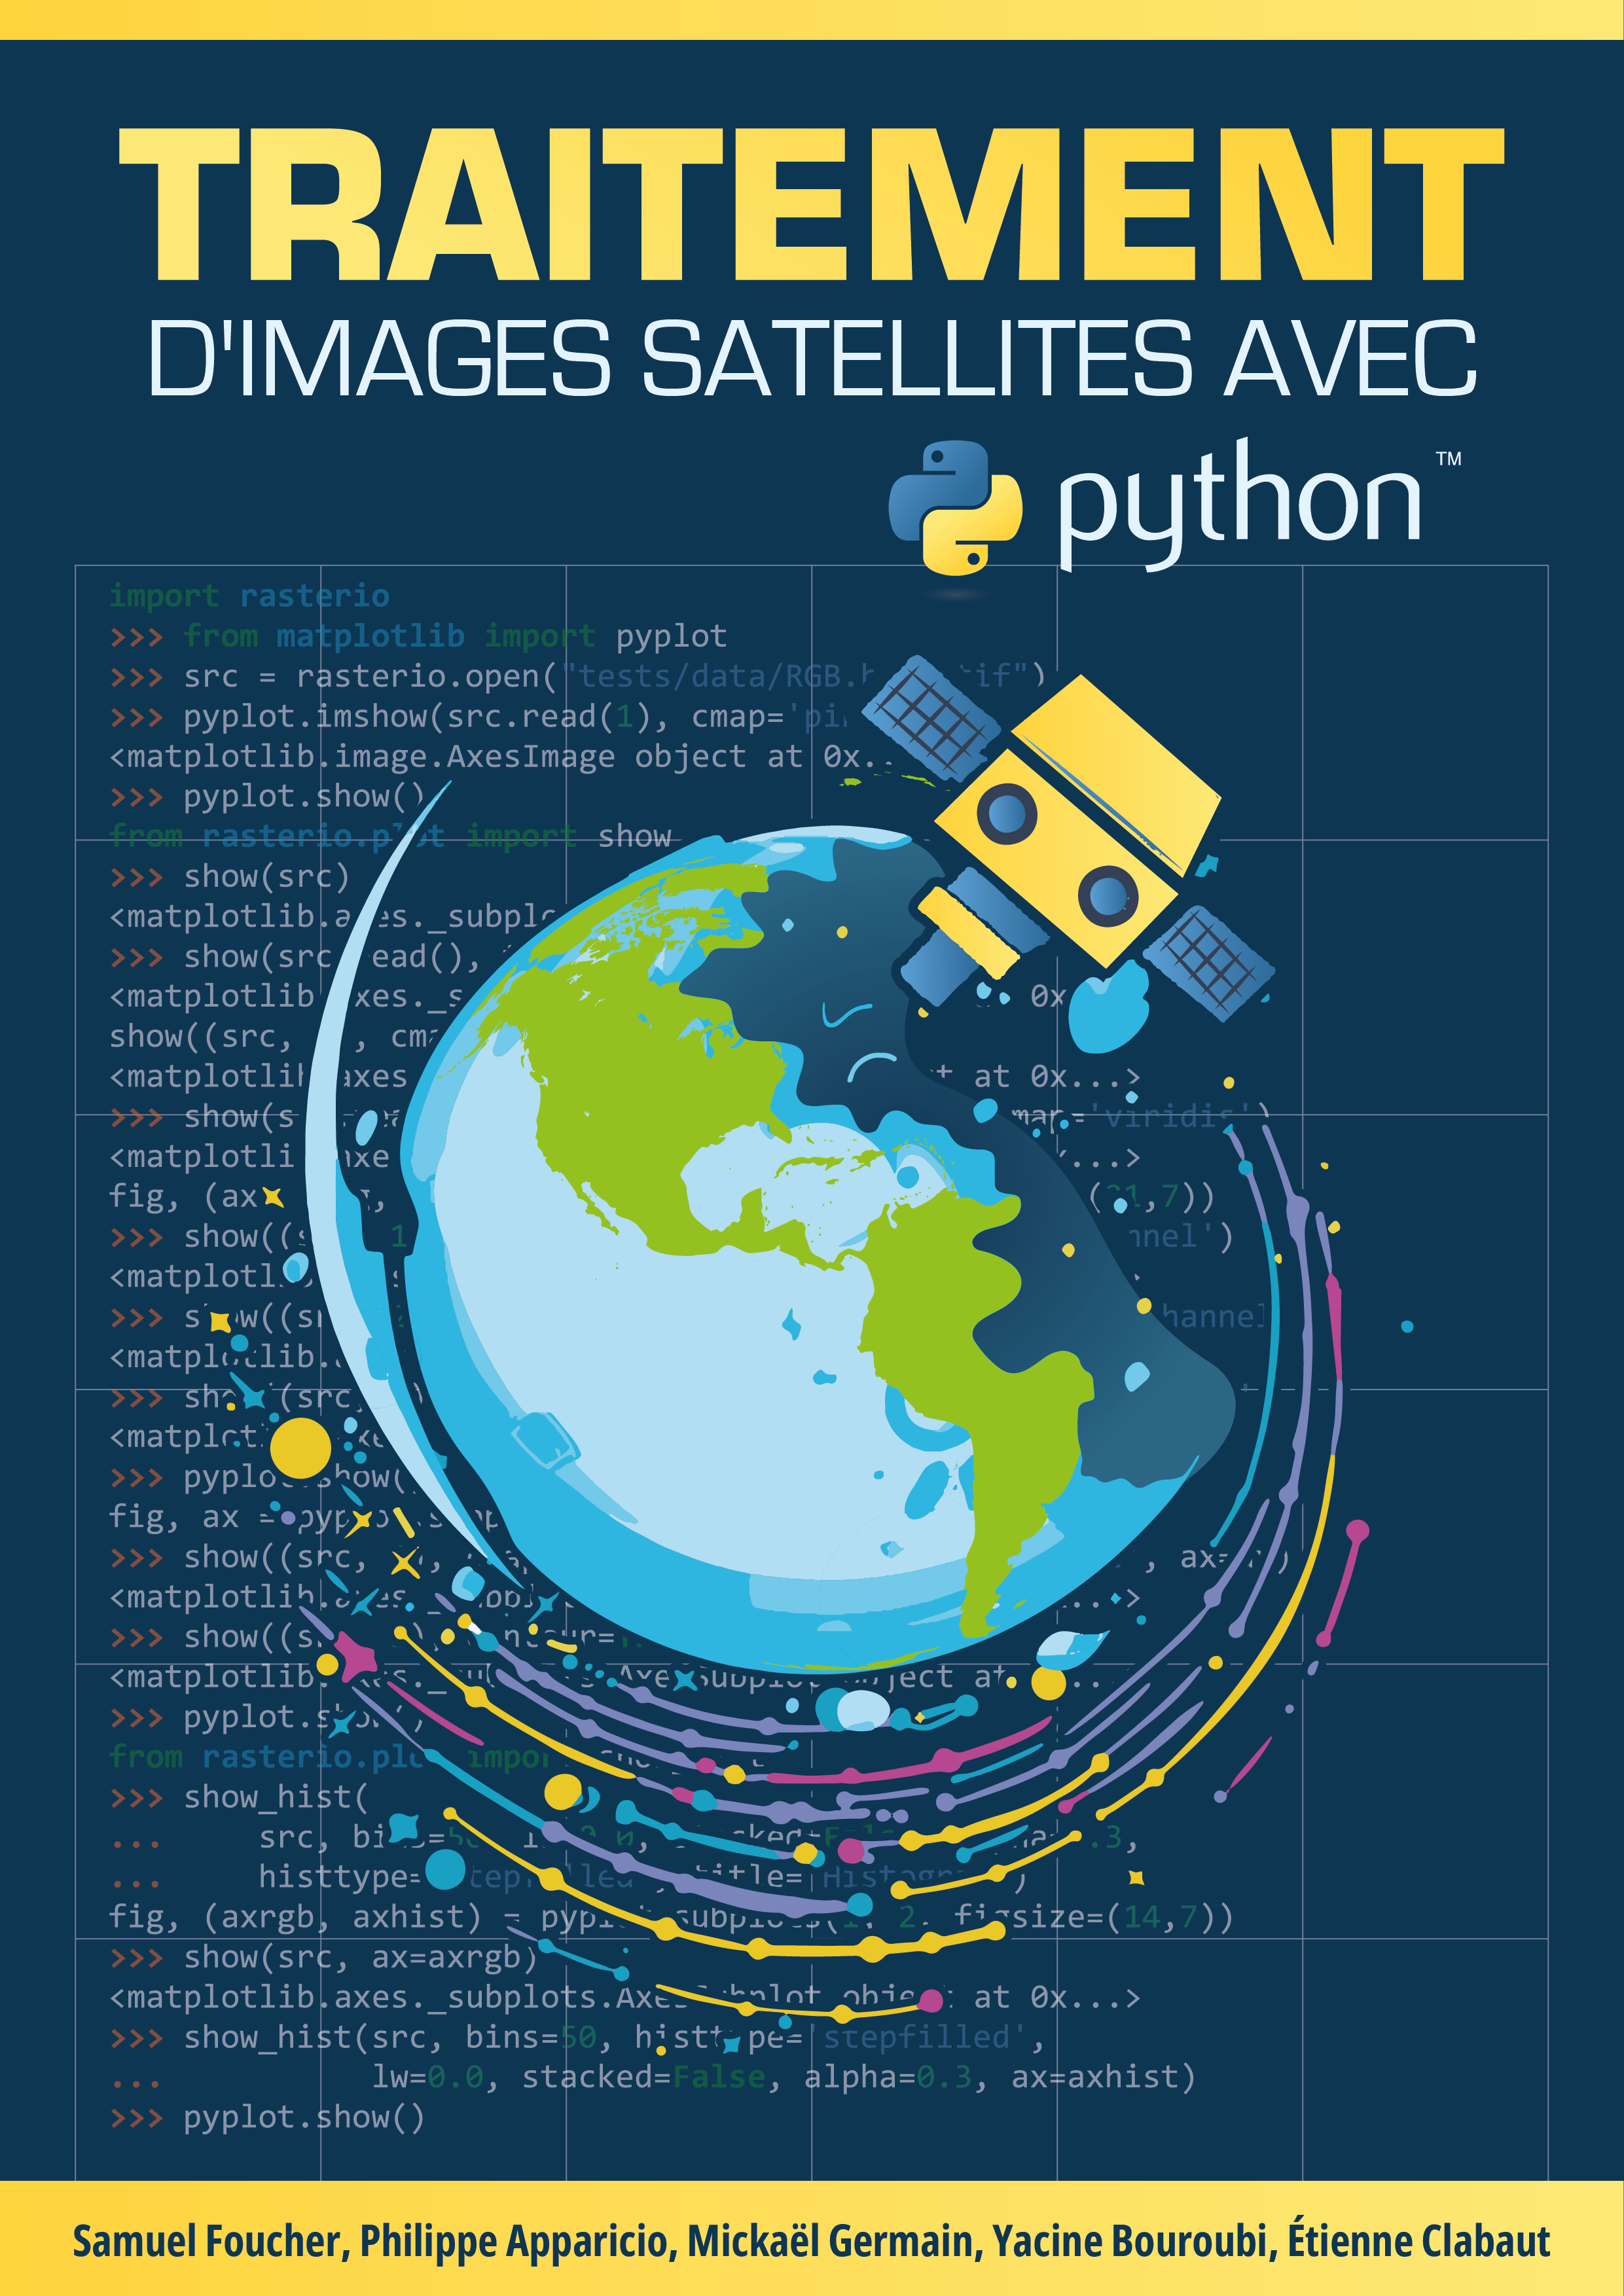
\includegraphics[width=4in]{images/couverture-full.png}}
\usepackage{xparse}
\usepackage{tcolorbox}
\usepackage{fvextra}
\DefineVerbatimEnvironment{Highlighting}{Verbatim}{numbers=left,breaklines=true,breakanywhere,commandchars=\\\{\}}
\let\oldverbatim\verbatim
\let\oldendverbatim\endverbatim
\DefineVerbatimEnvironment{verbatim}{Verbatim}{fontsize=\tiny,breaklines=true,fontfamily=courier}

\definecolor{package_color}{HTML}{e2e1f2}
\definecolor{objectif_color}{HTML}{e2efec}
\definecolor{notes_color}{HTML}{eef5fb}
\definecolor{allerloin_color}{HTML}{fcf7de}
\definecolor{astuce_color}{HTML}{f0f6ec}
\definecolor{attention_color}{HTML}{fef4ec}
\definecolor{exercise_color}{HTML}{fbe8f2}
\definecolor{background_color}{HTML}{FAF9FF}
\pdfminorversion=5
\pdfcompresslevel=9
\pdfobjcompresslevel=9
\usepackage{xparse}
\renewcommand{\thepart}{} % Enlever numérotation des parties
\setcounter{secnumdepth}{3} % Activer la numérotation des sections jusqu'au niveau des sous-sections
\makeatletter
\@ifpackageloaded{bookmark}{}{\usepackage{bookmark}}
\makeatother
\makeatletter
\@ifpackageloaded{caption}{}{\usepackage{caption}}
\AtBeginDocument{%
\ifdefined\contentsname
  \renewcommand*\contentsname{Table des matières}
\else
  \newcommand\contentsname{Table des matières}
\fi
\ifdefined\listfigurename
  \renewcommand*\listfigurename{Liste des Figures}
\else
  \newcommand\listfigurename{Liste des Figures}
\fi
\ifdefined\listtablename
  \renewcommand*\listtablename{Liste des Tables}
\else
  \newcommand\listtablename{Liste des Tables}
\fi
\ifdefined\figurename
  \renewcommand*\figurename{Figure}
\else
  \newcommand\figurename{Figure}
\fi
\ifdefined\tablename
  \renewcommand*\tablename{Tableau}
\else
  \newcommand\tablename{Tableau}
\fi
}
\@ifpackageloaded{float}{}{\usepackage{float}}
\floatstyle{ruled}
\@ifundefined{c@chapter}{\newfloat{codelisting}{h}{lop}}{\newfloat{codelisting}{h}{lop}[chapter]}
\floatname{codelisting}{Bloc

de

code}
\newcommand*\listoflistings{\listof{codelisting}{Liste des Listings}}
\makeatother
\makeatletter
\makeatother
\makeatletter
\@ifpackageloaded{caption}{}{\usepackage{caption}}
\@ifpackageloaded{subcaption}{}{\usepackage{subcaption}}
\makeatother

\ifLuaTeX
\usepackage[bidi=basic]{babel}
\else
\usepackage[bidi=default]{babel}
\fi
\babelprovide[main,import]{french}
% get rid of language-specific shorthands (see #6817):
\let\LanguageShortHands\languageshorthands
\def\languageshorthands#1{}
\usepackage{bookmark}

\IfFileExists{xurl.sty}{\usepackage{xurl}}{} % add URL line breaks if available
\urlstyle{same} % disable monospaced font for URLs
\hypersetup{
  pdftitle={Traitement d'images satellites avec Python},
  pdfauthor={Samuel Foucher; Philippe Apparicio; Yacine Bouroubi; Mickaël Germain; Étienne Clabaut},
  pdflang={fr},
  colorlinks=true,
  linkcolor={violet},
  filecolor={Maroon},
  citecolor={violet},
  urlcolor={Green4},
  pdfcreator={LaTeX via pandoc}}


\title{Traitement d'images satellites avec Python}
\usepackage{etoolbox}
\makeatletter
\providecommand{\subtitle}[1]{% add subtitle to \maketitle
  \apptocmd{\@title}{\par {\large #1 \par}}{}{}
}
\makeatother
\subtitle{Première édition}
\author{Samuel Foucher \and Philippe Apparicio \and Yacine
Bouroubi \and Mickaël Germain \and Étienne Clabaut}
\date{2025-03-22}

\begin{document}
\frontmatter
\maketitle

\renewcommand*\contentsname{Table des matières}
{
\hypersetup{linkcolor=}
\setcounter{tocdepth}{2}
\tableofcontents
}
\listoffigures
\listoftables

\mainmatter
\bookmarksetup{startatroot}

\chapter*{Préface}\label{pruxe9face}
\addcontentsline{toc}{chapter}{Préface}

\markboth{Préface}{Préface}

\renewcommand{\partname}{}

\% Réinitialiser partie

\textbf{Résumé~:} Ce livre vise à décrire une panoplie de méthodes de
traitement d'images satellites avec le langage Python. Celles et ceux
souhaitant migrer progressivement d'un autre logiciel d'imagerie et de
télédétection vers Python trouveront dans cet ouvrage les éléments pour
une transition en douceur. La philosophie de ce livre est de donner
toutes les clefs de compréhension et de mise en œuvre des méthodes
abordées dans Python. La présentation des méthodes est basée sur une
approche compréhensive et intuitive plutôt que mathématique, sans pour
autant négliger la rigueur mathématique ou statistique. Des rappels sur
les fondements en télédétection pourront apparaître au besoin afin
d'éclairer les approches techniques. Plusieurs éditions régulières sont
prévues sachant que ce domaine évolue constamment.

\textbf{Ce projet est en cours d'écriture et le contenu n'est pas
complet}


\includegraphics[width=0.5\linewidth,height=\textheight,keepaspectratio]{images/logos/under-construction-2408062_640.png}\hfill

\textbf{Remerciements~:} Ce manuel a été réalisé avec le soutien de la
fabriqueREL. Fondée en 2019, la fabriqueREL est portée par divers
établissements d'enseignement supérieur du Québec et agit en
collaboration avec les services de soutien pédagogique et les
bibliothèques. Son but est de faire des ressources éducatives libres
(REL) le matériel privilégié en enseignement supérieur au Québec.

\textbf{Mise en page~:} Samuel Foucher, Philippe Apparicio et
Marie-Hélène Gadbois Del Carpio.

© Samuel Foucher, Philippe Apparicio, Yacine Bouroubi et Mickaël
Germain.

\textbf{Pour citer cet ouvrage~:} Foucher S., Apparicio P., Bouroubi Y.,
Germain M. et Clabaut, E. (2025). \emph{Traitement d'images satellites
avec Python}. Université de Sherbrooke, Département de géomatique
appliquée. fabriqueREL. Licence CC~BY-SA.


\includegraphics[width=0.8\linewidth,height=\textheight,keepaspectratio]{images/introduction/CouvertureP2.png}\hfill

\section*{Un manuel sous la forme d'une ressource éducative
libre}\label{sect001}
\addcontentsline{toc}{section}{Un manuel sous la forme d'une ressource
éducative libre}

\markright{Un manuel sous la forme d'une ressource éducative libre}

\textbf{Pourquoi un manuel sous licence libre?}

Les logiciels libres sont aujourd'hui très répandus. Comparativement aux
logiciels propriétaires, l'accès au code source permet à quiconque de
l'utiliser, de le modifier, de le dupliquer et de le partager. Le
logiciel Python, dans lequel sont mises en œuvre les méthodes de
traitement d'images satellites décrites dans ce livre, est d'ailleurs à
la fois un langage de programmation et un logiciel libre (sous la
licence publique générale
\href{https://fr.wikipedia.org/wiki/Licence_publique_g\%C3\%A9n\%C3\%A9rale_GNU}{GNU
GPL2}). Par analogie aux logiciels libres, il existe aussi des
\textbf{ressources éducatives libres (REL)} «~dont la licence accorde
les permissions désignées par les 5R (\textbf{Retenir --- Réutiliser ---
Réviser --- Remixer --- Redistribuer}) et donc permet nécessairement la
modification~»
(\href{https://fabriquerel.org/rel/}{\textbf{\emph{fabriqueREL}}}). La
licence de ce livre, CC BY-SA (figure~\ref{fig-Licence}), permet donc
de~:

\begin{itemize}
\item
  \textbf{Retenir}, c'est-à-dire télécharger et imprimer gratuitement le
  livre. Notez qu'il aurait été plutôt surprenant d'écrire un livre
  payant sur un logiciel libre et donc gratuit. Aussi, nous aurions été
  très embarrassés que des personnes étudiantes avec des ressources
  financières limitées doivent payer pour avoir accès au livre, sans
  pour autant savoir préalablement si le contenu est réellement adapté à
  leurs besoins.
\item
  \textbf{Réutiliser}, c'est-à-dire utiliser la totalité ou une section
  du livre sans limitation et sans compensation financière. Cela permet
  ainsi à d'autres personnes enseignantes de l'utiliser dans le cadre
  d'activités pédagogiques.
\item
  \textbf{Réviser}, c'est-à-dire modifier, adapter et traduire le
  contenu en fonction d'un besoin pédagogique précis puisqu'aucun manuel
  n'est parfait, tant s'en faut! Le livre a d'ailleurs été écrit
  intégralement dans Python avec \href{https://quarto.org/}{Quatro}.
  Quiconque peut ainsi télécharger gratuitement le code source du livre
  sur
  \href{https://github.com/serie-python-tele/TraitementImagesPythonVol1}{GitHub}
  et le modifier à sa guise (voir l'encadré intitulé \emph{Suggestions
  d'adaptation du manuel}).
\item
  \textbf{Remixer}, c'est-à-dire «~combiner la ressource avec d'autres
  ressources dont la licence le permet aussi pour créer une nouvelle
  ressource intégrée~»
  (\href{https://fabriquerel.org/rel/}{\textbf{\emph{fabriqueREL}}}).
\item
  \textbf{Redistribuer}, c'est-à-dire distribuer, en totalité ou en
  partie le manuel ou une version révisée sur d'autres canaux que le
  site Web du livre (par exemple, sur le site Moodle de votre université
  ou en faire une version imprimée).
\end{itemize}

La licence de ce livre, CC BY-SA (figure~\ref{fig-Licence}), oblige donc
à~:

\begin{itemize}
\tightlist
\item
  Attribuer la paternité de l'auteur dans vos versions dérivées, ainsi
  qu'une mention concernant les grandes modifications apportées, en
  utilisant la formulation suivante~:
\end{itemize}

Samuel Foucher, Apparicio Philippe, Mickaël Germain, Yacine Bouroubi et
Étienne Clabaut (2025). \emph{Traitement d'images satellites avec
Python}. Université de Sherbrooke, Département de géomatique appliquée.
fabriqueREL. Licence CC~BY-SA.

\begin{itemize}
\tightlist
\item
  Utiliser la même licence ou une licence similaire à toutes versions
  dérivées.
\end{itemize}

\begin{figure}

\centering{

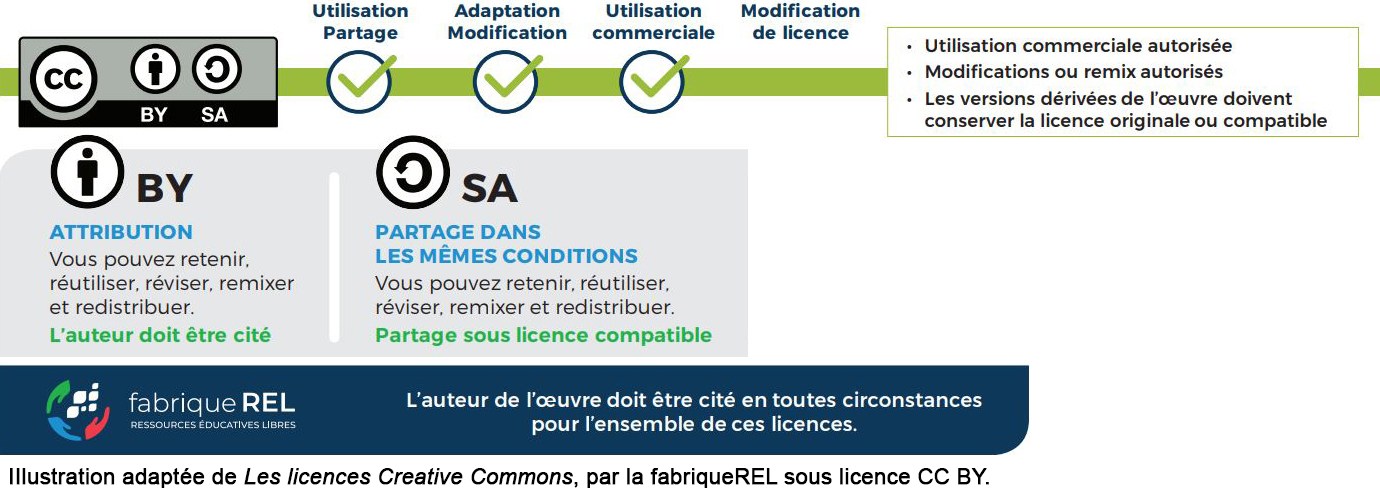
\includegraphics[width=0.8\linewidth,height=\textheight,keepaspectratio]{images/introduction/Licence.JPG}

}

\caption{\label{fig-Licence}Licence Creative Commons du livre}

\end{figure}%

\begin{tcolorbox}[colback=background_color, colframe=astuce_color, boxrule=0.2mm, leftrule=1mm, coltitle=black, fonttitle=\bfseries, title={
\includegraphics[width=0.3cm]{images/BlocAstuce.png} \textbf{Astuce}}]

\textbf{Suggestions d'adaptation du manuel}

Pour chaque méthode de traitement d'image abordée dans le livre, une
description détaillée et une mise en œuvre dans Python sont disponibles.
Par conséquent, plusieurs adaptations du manuel sont possibles~:

\begin{itemize}
\item
  Conserver uniquement les chapitres sur les méthodes ciblées dans votre
  cours.
\item
  En faire une version imprimée et la distribuer aux personnes
  étudiantes.
\item
  Modifier la description d'une ou de plusieurs méthodes en effectuant
  les mises à jour directement dans les chapitres.
\item
  Insérer ses propres jeux de données dans les sections intitulées
  \emph{Mise en œuvre dans Python}.
\item
  Modifier les tableaux et figures.
\item
  Ajouter une série d'exercices.
\item
  Modifier les quiz de révision.
\item
  Rédiger un nouveau chapitre.
\item
  Modifier des syntaxes en Python. Plusieurs \emph{librairies} Python
  peuvent être utilisées pour mettre en œuvre telle ou telle méthode.
  Ces derniers évoluent aussi très vite et de nouvelles
  \emph{librairies} sont proposées fréquemment! Par conséquent, il peut
  être judicieux de modifier une syntaxe Python du livre en fonction de
  ses habitudes de programmation en Python (utilisation d'autres
  \emph{librairies} que ceux utilisés dans le manuel par exemple) ou de
  bien mettre à jour une syntaxe à la suite de la parution d'une
  nouvelle \emph{librairie} plus performante ou intéressante.
\item
  Toute autre adaptation qui permet de répondre au mieux à un besoin
  pédagogique.
\end{itemize}

\end{tcolorbox}

\section*{Comment lire ce manuel?}\label{sect002}
\addcontentsline{toc}{section}{Comment lire ce manuel?}

\markright{Comment lire ce manuel?}

Le livre comprend plusieurs types de blocs de texte qui en facilitent la
lecture.

\begin{tcolorbox}[colback=background_color, colframe=package_color, boxrule=0.2mm, leftrule=1mm, coltitle=black, fonttitle=\bfseries, title={
\includegraphics[width=0.3cm]{images/BlocPackage.png} \textbf{Package}}]

\textbf{Bloc \emph{packages}}

Habituellement localisé au début d'un chapitre, il comprend la liste des
\emph{packages} Python utilisés pour un chapitre.

\end{tcolorbox}

\begin{tcolorbox}[colback=background_color, colframe=objectif_color, boxrule=0.2mm, leftrule=1mm, coltitle=black, fonttitle=\bfseries, title={
\includegraphics[width=0.3cm]{images/BlocObjectif.png} \textbf{Objectif}}]

\textbf{Bloc objectif}

Il comprend une description des objectifs d'un chapitre ou d'une
section.

\end{tcolorbox}

\begin{tcolorbox}[colback=background_color, colframe=notes_color, boxrule=0.2mm, leftrule=1mm, coltitle=black, fonttitle=\bfseries, title={
\includegraphics[width=0.3cm]{images/BlocNote.png} \textbf{Note}}]

\textbf{Bloc notes}

Il comprend une information secondaire sur une notion, une idée abordée
dans une section.

\end{tcolorbox}

\begin{tcolorbox}[colback=background_color, colframe=allerloin_color, boxrule=0.2mm, leftrule=1mm, coltitle=black, fonttitle=\bfseries, title={
\includegraphics[width=0.3cm]{images/BlocAllerPlusLoin.png} \textbf{Aller plus loin}}]

\textbf{Bloc pour aller plus loin}

Il comprend des références ou des extensions d'une méthode abordée dans
une section.

\end{tcolorbox}

\begin{tcolorbox}[colback=background_color, colframe=astuce_color, boxrule=0.2mm, leftrule=1mm, coltitle=black, fonttitle=\bfseries, title={
\includegraphics[width=0.3cm]{images/BlocAstuce.png} \textbf{Astuce}}]

\textbf{Bloc astuce}

Il décrit un élément qui vous facilitera la vie~: une propriété
statistique, un \emph{package}, une fonction, une syntaxe Python.

\end{tcolorbox}

\begin{tcolorbox}[colback=background_color, colframe=attention_color, boxrule=0.2mm, leftrule=1mm, coltitle=black, fonttitle=\bfseries, title={
\includegraphics[width=0.3cm]{images/BlocAttention.png} \textbf{Attention}}]

\textbf{Bloc attention}

Il comprend une notion ou un élément important à bien maîtriser.

\end{tcolorbox}

\begin{tcolorbox}[colback=background_color, colframe=exercise_color, boxrule=0.2mm, leftrule=1mm, coltitle=black, fonttitle=\bfseries, title={
\includegraphics[width=0.3cm]{images/BlocExercice.png} \textbf{Exercice}}]

\textbf{Bloc exercice}

Il comprend un court exercice de révision à la fin de chaque chapitre.

\end{tcolorbox}

\section*{Comment utiliser les données du livre pour reproduire les
exemples?}\label{sect003}
\addcontentsline{toc}{section}{Comment utiliser les données du livre
pour reproduire les exemples?}

\markright{Comment utiliser les données du livre pour reproduire les
exemples?}

Ce livre comprend des exemples détaillés et appliqués en Python pour
chacune des méthodes abordées. Ces exemples se basent sur des jeux de
données ouverts et mis à disposition avec le livre. Ils sont disponibles
sur le \emph{repo GitHub} dans le sous-dossier \texttt{data}, à
l'adresse
\url{https://github.com/serie-tele-pyton/TraitementImagesVol1/tree/main/data}.

Une autre option est de télécharger le \emph{repo} complet du livre
directement sur \emph{GitHub}
(\url{https://github.com/serie-tele-pyton/TraitementImagesVol1}) en
cliquant sur le bouton \texttt{Code}, puis le bouton
\texttt{Download\ ZIP} (figure~\ref{fig-downloaffromgit}). Les données
se trouvent alors dans le sous-dossier nommé \texttt{data}.

\begin{figure}

\centering{

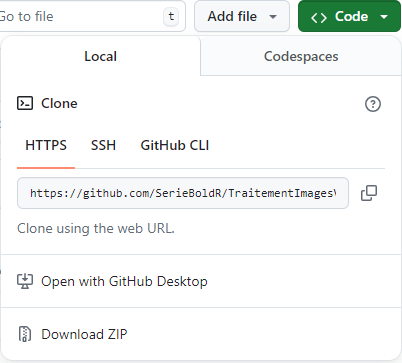
\includegraphics[width=0.4\linewidth,height=\textheight,keepaspectratio]{images/introduction/download_github.png}

}

\caption{\label{fig-downloaffromgit}Téléchargement de l'intégralité du
livre}

\end{figure}%

\section*{Structure du livre}\label{sect004}
\addcontentsline{toc}{section}{Structure du livre}

\markright{Structure du livre}

Le livre est organisé autour de quatre grandes parties.

\textbf{Partie 1. Importation et manipulation de données spatiales.}
Dans cette première partie, nous voyons comment importer, manipuler,
visualiser et exporter des données spatiales de type image (ou de type
matriciel) avec Python, principalement avec les \emph{packages}
\texttt{rasterio}, \texttt{xarray} et \texttt{numpy}
(chapitre~\ref{sec-chap01}). Ce chapitre vous permettra de maîtriser la
manipulation à bas niveau de différents types d'imagerie. Différents
exemples et exercises sont disponibles avec différents capteurs
satellites (multi-spectral, RGB-NIR, SAR, etc.)

\textbf{Partie 2. Transformations des données spatiales}. Cette deuxième
partie comprend deux chapitres~: les transformations spectrales
(chapitre~\ref{sec-chap03}) et les transformations spatiales
(chapitre~\ref{sec-chap04}).

\textbf{Partie 3. Classifications d'images.} Cette troisième partie
comprend deux chapitres~: les classifications supervisées
(chapitre~\ref{sec-chap05}) et non supervisées (à venir dans une
prochaine édition).

\textbf{Partie 4. Données massives.} (à venir dans une édition future).
Cette quatrième et dernière partie comprend un seul chapitre qui est
dédié aux plateformes de mégadonnées, notamment Google Earth Engine.

\section*{Remerciements}\label{sect005}
\addcontentsline{toc}{section}{Remerciements}

\markright{Remerciements}

De nombreuses personnes ont contribué à l'élaboration de ce manuel.

Ce projet a bénéficié du soutien pédagogique et financier de la
\href{https://fabriquerel.org/}{\textbf{\emph{fabriqueREL}}} (ressources
éducatives libres). Les différentes rencontres avec le comité de suivi
nous ont permis de comprendre l'univers des ressources éducatives libres
(REL) et notamment leurs \href{https://fabriquerel.org/rel/}{fameux 5R}
(Retenir --- Réutiliser --- Réviser --- Remixer --- Redistribuer), de
mieux définir le besoin pédagogique visé par ce manuel, d'identifier des
ressources pédagogiques et des outils pertinents pour son élaboration.
Ainsi, nous remercions chaleureusement les membres de la
\emph{fabriqueREL} pour leur soutien inconditionnel~:

\begin{itemize}
\item
  José-Miguel Escobar-Zuniga, bibliothécaire à l'Université de
  Sherbrooke.
\item
  Marianne Dubé, coordonnatrice de la fabriqueREL, Université de
  Sherbrooke.
\item
  Claude Potvin, conseiller en formation, Service de soutien à
  l'enseignement, Université Laval.
\end{itemize}

Nous remercions chaleureusement les personnes étudiantes du
\href{https://www.usherbrooke.ca/admission/programme/271/baccalaureat-en-geomatiqueappliquee-a-lenvironnement/}{Baccalauréat
en géomatique appliquée à l'environnement} et du
\href{https://www.usherbrooke.ca/admission/programme/429/microprogramme-de-1er-cycleen-geomatique-appliquee/}{Microprogramme
de 1er cycle en géomatique appliquée} du
\href{https://www.usherbrooke.ca/geomatique/}{Département de géomatique
appliquée} de l'\href{https://www.usherbrooke.ca/}{Université de
Sherbrooke} qui utilisent le manuel dans le cadre de cours.

\section*{Introduction aux images de télédétection}\label{sect006}
\addcontentsline{toc}{section}{Introduction aux images de télédétection}

\markright{Introduction aux images de télédétection}

L'imagerie numérique a pris une place importante dans notre vie de tous
les jours depuis une quinzaine d'années. Ces images sont prises
généralement au niveau du sol (imagerie proximale) avec seulement trois
couleurs dans le domaine de la vision humaine (rouge, vert et bleu).
Dans la suite du manuel, on parlera d'images du domaine de la vision par
ordinateur ou images en vision pour faire plus court.

Les images de télédétection ont des particularités et des propriétés qui
les différencient des images ``classiques'', dont les cinq principales
sont:

\begin{enumerate}
\def\labelenumi{\arabic{enumi}.}
\item
  Les images sont géoréférencées. Cela signifie que pour chaque pixel
  nous pouvons y associer une position géographique ou cartographique.
\item
  Le point de vue est très différent. Ces images sont prises avec une
  vue d'en haut (Nadir) ou oblique avec une distance qui peut être très
  grande; on parle d'images distales.
\item
  Elles possèdent plus que 3 bandes. Contrairement aux images en vision,
  les images de télédétection possèdent bien souvent plus que trois
  bandes. Il n'est pas rare de trouver quatre bandes (Pléiade), 13
  bandes (Sentinel-2, Landsat) et même 200 bandes pour des capteurs
  hyperspectraux.
\item
  Elles peuvent être calibrées. Les valeurs numérique de l'image peuvent
  être converties en quantités physiques (luminance, réflectance,
  section efficace, etc.) via une fonction de calibration.
\item
  Elles sont de grande taille. Il n'est pas rare de manipuler des images
  qui font plusieurs dizaines de milliers de pixels en dimension.
\end{enumerate}

\subsection*{Ressources en ligne}\label{ressources-en-ligne}
\addcontentsline{toc}{subsection}{Ressources en ligne}

\subsection*{\texorpdfstring{Listes des \emph{librairies}
utilisés}{Listes des librairies utilisés}}\label{sect0071}
\addcontentsline{toc}{subsection}{Listes des \emph{librairies} utilisés}

Dans ce livre, nous utilisons de nombreux \emph{packages} Python que
vous pouvez installer en une seule fois (voir section~\ref{sec-00-01})
ou chapitre par chapitre.

\bookmarksetup{startatroot}

\chapter*{À propos des auteurs}\label{auteurs}
\addcontentsline{toc}{chapter}{À propos des auteurs}

\markboth{À propos des auteurs}{À propos des auteurs}

\href{https://www.usherbrooke.ca/recherche/fr/specialistes/details/samuel.foucher}{\textbf{Samuel
Foucher}} est professeur au
\href{https://www.usherbrooke.ca/geomatique/}{Département de géomatique
appliquée} de l'\href{https://www.usherbrooke.ca/}{Université de
Sherbrooke}. Il y enseigne aux
\href{https://www.usherbrooke.ca/geomatique/etudes/programmes}{programmes
de 1\textsuperscript{er} et 2\textsuperscript{e} cycles de géomatique}
les cours \emph{Traitement numérique des images de télédétection},
\emph{Base de données géospatiales} et \emph{Apprentissage profond
appliqué à l'observation de la Terre}. Ses intérêts de recherche portent
sur le traitement d'images et l'application de l'IA aux données
géospatiales.

\href{https://www.usherbrooke.ca/recherche/fr/specialistes/details/philippe.apparicio}{\textbf{Philippe
Apparicio}} est professeur titulaire au
\href{https://www.usherbrooke.ca/geomatique/}{Département de géomatique
appliquée} de l'\href{https://www.usherbrooke.ca/}{Université de
Sherbrooke}. Il y enseigne aux
\href{https://www.usherbrooke.ca/geomatique/etudes/programmes}{programmes
de 1\textsuperscript{er} et 2\textsuperscript{e} cycles de géomatique}
les cours \emph{Transport et mobilité durable}, \emph{Modélisation et
analyse spatiale} et \emph{Géomatique appliquée à la gestion urbaine}.
Durant les dernières années, il a offert plusieurs formations aux Écoles
d'été du Centre interuniversitaire québécois de statistiques sociales
(\href{https://www.ciqss.org/}{CIQSS}). Géographe de formation, ses
intérêts de recherche incluent la justice et l'équité environnementale,
la mobilité durable, les pollutions atmosphérique et sonore, et le vélo
en ville. Il a publié une centaine d'articles scientifiques dans
différents domaines des études urbaines et de la géographie mobilisant
la géomatique et l'analyse spatiale.

\href{https://www.usherbrooke.ca/geomatique/departement/personnel/personnel-enseignant/mickael-germain}{\textbf{Mickaël
Germain}} est professeur agrégé au
\href{https://www.usherbrooke.ca/geomatique/}{Département de géomatique
appliquée} de l'\href{https://www.usherbrooke.ca/}{Université de
Sherbrooke}.

\href{https://www.usherbrooke.ca/geomatique/departement/personnel/personnel-enseignant/yacine-bouroubi}{\textbf{Yacine
Bouroubi}} est professeur agrégé au
\href{https://www.usherbrooke.ca/geomatique/}{Département de géomatique
appliquée} de l'\href{https://www.usherbrooke.ca/}{Université de
Sherbrooke}.

\href{https://www.linkedin.com/in/\%C3\%A9tienne-clabaut-793a4176/?originalSubdomain=ca}{\textbf{Étienne
Clabaut}} est professeur associé au
\href{https://www.usherbrooke.ca/geomatique/}{Département de géomatique
appliquée} de l'\href{https://www.usherbrooke.ca/}{Université de
Sherbrooke}.

\part{Partie 1. Importation, manipulation et visualisation de données
spatiales}

\bookmarksetup{startatroot}

\chapter{Introduction au langage Python}\label{sec-chap00}

Dans ce chapitre, nous présentons quelques éléments essentiels du
langage Python qui nous seront utiles dans ce manuel. Python est un
langage très riche et peut aboutir à des projets logiciels très
sophistiqués. Il est important de comprendre que la programmation Python
n'est pas ici une fin en soi, mais plutôt un outil de scriptage et de
manipulation des données satellitaires.

\begin{tcolorbox}[colback=background_color, colframe=objectif_color, boxrule=0.2mm, leftrule=1mm, coltitle=black, fonttitle=\bfseries, title={
\includegraphics[width=0.3cm]{images/BlocObjectif.png} \textbf{Objectif}}]

\textbf{Objectifs d'apprentissage visés dans ce chapitre}

À la fin de ce chapitre, vous devriez être en mesure de~:

\begin{itemize}
\tightlist
\item
  connaître les principales distributions de Python;
\item
  installer un environnement d'exécution du code de cet ouvrage;
\item
  comprendre les structures de base du langage Python;
\end{itemize}

\end{tcolorbox}

Python, créé par
\href{https://en.wikipedia.org/wiki/Guido_van_Rossum}{Guido van Rossum}
en 1991, est un langage de programmation polyvalent et facile à
apprendre, souvent comparé à un couteau suisse numérique pour sa
simplicité et sa polyvalence. Comme un outil multifonction, Python peut
être utilisé pour une variété de tâches, du développement web à
l'analyse de données, en passant par l'intelligence artificielle.

\section{Les distributions}\label{les-distributions}

Il existe plusieurs
\href{https://wiki.python.org/moin/PythonDistributions}{distributions}
du langage Python, ces distributions sont comme différentes saveurs de
votre glace préférée - chacune a ses propres caractéristiques uniques,
mais elles sont toutes fondamentalement Python. Voici un aperçu des
principales distributions :

\begin{itemize}
\item
  \href{https://www.python.org/downloads/}{CPython} est la distribution
  ``vanille'' officielle, comme la recette originale de Python. Elle est
  ainsi le choix idéal pour la compatibilité et la conformité aux
  standards.
\item
  \href{https://www.anaconda.com/download}{Anaconda}. Pensez-y comme à
  un sundae tout garni. Elle vient avec de nombreuses bibliothèques
  scientifiques préinstallées, ce qui est idéal pour l'analyse de
  données et l'apprentissage automatique (\emph{machine learning}).
\item
  \href{https://docs.anaconda.com/miniconda/miniconda-install/}{Miniconda}
  est une distribution légère de Python qui vous permet d'ajouter au
  besoin d'autres bibliothèques.
\item
  \href{https://pypy.org/}{PyPy} : est une version turbo de Python,
  optimisée pour la vitesse.
\end{itemize}

Chaque distribution a ses forces, que ce soit la simplicité, la vitesse
ou des fonctionnalités spécifiques. Le choix dépend donc de vos besoins,
comme choisir entre une glace simple ou une glace royal (banana split)
élaboré.

\section{Les styles de programmation en
Python}\label{les-styles-de-programmation-en-python}

Il existe plusieurs approches pour programmer en Python. La plus directe
est en version interactive en tapant \texttt{python} et de rentrer des
commandes ligne par ligne.

\subsection{Les outils de
programmation}\label{les-outils-de-programmation}

Un code python prend la forme d'un simple fichier texte avec l'extension
\texttt{.py} et peut être modifié avec un simple éditeur de texte.
Cependant, il n'y aura pas de rétroactions immédiates de l'interpréteur
Python, ce qui rend la correction d'erreurs (débogage) beaucoup plus
laborieux.

Un IDE (\emph{Integrated Developement Environnement}) est comme une
boîte à outils complète pour les programmeurs, vous trouverez :

\begin{itemize}
\item
  Un éditeur de texte amélioré pour écrire votre code, avec des
  fonctionnalités comme la coloration syntaxique qui rend le code plus
  lisible.
\item
  Un compilateur qui transforme votre code en instructions que
  l'ordinateur peut comprendre.
\item
  Un débogueur pour trouver et corriger les erreurs, tel un détective
  numérique.
\item
  Des outils d'automatisation qui effectuent des tâches répétitives,
  comme un assistant virtuel pour le codage.
\item
  L'accès à la documentation des différentes librairies.
\end{itemize}

Ces outils intégrés permettent aux développeurs de travailler plus
efficacement, en passant moins de temps à jongler entre différentes
applications et plus de temps à produire du code.

Voici quelques options populaires :

\begin{itemize}
\item
  \href{https://www.jetbrains.com/pycharm/}{PyCharm}: est un des outils
  les plus utilisés dans l'industrie. Il offre une multitude de
  fonctionnalités comme l'autocomplétion intelligente et le débogage
  intégré, idéal pour les grands projets. Cependant, cet outil peut être
  assez gourmand en mémoire et en CPU. Notez qu'il existe une version
  gratuite et une version professionnelle.
\item
  \href{https://code.visualstudio.com/}{Visual Studio Code} : gratuit,
  léger mais puissant, il est personnalisable avec des extensions pour
  Python.
\item
  \href{https://www.spyder-ide.org/}{Spyder} : logiciel libre et
  gratuit, orienté vers les applications scientifiques.
\item
  \href{https://jupyter.org/}{Jupyter Notebooks} : imaginez un cahier
  interactif pour le code. Idéal pour l'analyse de données et
  l'apprentissage, il permet de mélanger code, texte et visualisations.
  Des services gratuits dans le \textbf{cloud} sont disponibles comme
  Google Colab et Kaggle. Ces environnements sont néanmoins moins
  appropriés pour des grands projets et le débogage. Jupyter peut
  souffrir de problèmes de reproductibilité dus à l'exécution arbitraire
  des cellules.
\item
  \href{https://marimo.io/}{Marimo} se veut une version plus moderne des
  \emph{notebooks jupyter}. Contrairement à Jupyter, Marimo garantit la
  cohérence entre le code, les sorties et l'état du programme. Il
  analyse intelligemment les relations entre les cellules et réexécute
  automatiquement celles qui sont affectées par des changements,
  éliminant ainsi les problèmes d'état caché.
\end{itemize}

\section{Bonnes pratiques}\label{bonnes-pratiques}

Python est un langage très dynamique, qui évolue constamment. Cela pose
certains défis pour la gestion du code à long terme. Il est fortement
conseillé d'utiliser des environnements virtuels pour gérer vos
différentes bibliothèques (\emph{libraries}). Voici quelques bonnes
pratiques à suivre :

\begin{enumerate}
\def\labelenumi{\arabic{enumi}.}
\item
  \textbf{N'installez par la toute dernière version de Python} : Il est
  recommandé d'installer 1 ou 2 version antérieure, par exemple si 3.13
  est \href{https://www.python.org/downloads/}{la version plus récente},
  installer plutôt la version 3.11. Les versions trop récentes peuvent
  être instables. La version de python désirée peut être spécifiée au
  moment de la création d'un environnement virtuel (voir plus bas). Vous
  pouvez afficher la liste des versions de python avec la commande
  \texttt{conda\ search\ -\/-full-name\ python}.
\item
  \textbf{N'utilisez pas de version obsolète de Python}. Cela peut
  sembler contradictoire avec le point précédent mais c'est l'excès
  inverse. Si vous utilisez une version trop ancienne alors toutes vos
  librairies cesseront d'évoluer et peuvent devenir obsolètes.
\item
  \textbf{Utilisez des environnements virtuels}. Pensez-y comme à des
  compartiments séparées pour chaque projet. Cela évite les conflits
  entre les différentes versions de bibliothèques (\emph{libraries})et
  garde votre système propre. Par exemple, si vous souhaitez vérifier
  une nouvelle version de Python, utilisez un environnement :
  \texttt{conda\ create\ -\/-name\ test\ python=3.11}
\item
  \textbf{Vérifiez l'installation}. Après l'installation, ouvrez un
  terminal et tapez \texttt{python\ -\/-version} pour vous assurer que
  tout fonctionne correctement.
\end{enumerate}

\subsection{Création d'un environnement virtuel}\label{sec-00-01}

Il y a deux façons d'installer un environnement virtuel selon votre
distribution de Python:

\begin{enumerate}
\def\labelenumi{\arabic{enumi}.}
\tightlist
\item
  \textbf{Option 1}. Vous utilisez
  \href{https://www.anaconda.com/download}{Anaconda} ou
  \href{https://docs.anaconda.com/miniconda/miniconda-install/}{Miniconda}.
  La commande \texttt{conda} est utilisée pour créer un environnement
  test avec Python 3.10:
\end{enumerate}

\begin{Shaded}
\begin{Highlighting}[]
\ExtensionTok{conda}\NormalTok{ env }\AttributeTok{{-}n}\NormalTok{ test python=3.10}
\ExtensionTok{conda}\NormalTok{ activate test}
\end{Highlighting}
\end{Shaded}

\begin{enumerate}
\def\labelenumi{\arabic{enumi}.}
\setcounter{enumi}{1}
\tightlist
\item
  \textbf{Option 2}. Vous utilisez
  \href{https://www.python.org/downloads/}{CPython}
\end{enumerate}

\begin{Shaded}
\begin{Highlighting}[]
\ExtensionTok{conda}\NormalTok{ env }\AttributeTok{{-}n}\NormalTok{ test python=3.10}
\ExtensionTok{conda}\NormalTok{ activate test}
\end{Highlighting}
\end{Shaded}

\subsection{Création d'un environnement de travail local
(avancé)}\label{cruxe9ation-dun-environnement-de-travail-local-avancuxe9}

\textbf{Note}: les notebooks peuvent fonctionner localement uniquement
sous Linux ou avec WSL2.

Les notebooks Python fonctionnent par défaut dans l'environnement
\href{https://colab.google/}{Google Colab}. Si vous souhaitez faire
fonctionner ces notebook localement, vous pouvez installer un
environnement local avec un serveur
\href{https://jupyterlab.readthedocs.io/en/stable/getting_started/starting.html}{Jupyter}.
Il suffit de suivre les étapes suivantes:

1. Installer \texttt{WSL2} sous
\href{https://learn.microsoft.com/en-us/windows/wsl/install}{Windows}

2. Installer
\href{https://code.visualstudio.com/docs/setup/windows}{vscode}

3. Installer
\href{https://docs.anaconda.com/miniconda/install/\#quick-command-line-install}{Miniconda}

4. Faire une installation du contenu du livre soit en utilisant une
commande \texttt{git\ clone} ou en récupérant le \texttt{.zip} du livre

5. Ouvrir WSL2 et placer vous dans le répertoire du livre
\texttt{TraitementImagesPythonVol1}. Assurez vous que vous avez accès à
conda en tapant \texttt{conda\ -\/-version}

6. Lancer la commande \texttt{conda\ env\ create\ -f\ jupyter\_env.yaml}

7. Activer le nouvel environnement:
\texttt{conda\ activate\ jupyter\_env}

8. Le serveur jupyter peut ensuite être lancé avec la commande suivante:
\texttt{jupyter\ lab\ -\/-ip=\textquotesingle{}*\textquotesingle{}\ -\/-NotebookApp.token=\textquotesingle{}\textquotesingle{}\ -\/-NotebookApp.password=\textquotesingle{}\textquotesingle{}}

Une fenêtre devrait alors apparaître dans votre fureteur. Dans le menu
de gauche vous pouvez accéder aux notebooks dans le répertoire
\texttt{notebooks}:

\begin{figure}

\centering{

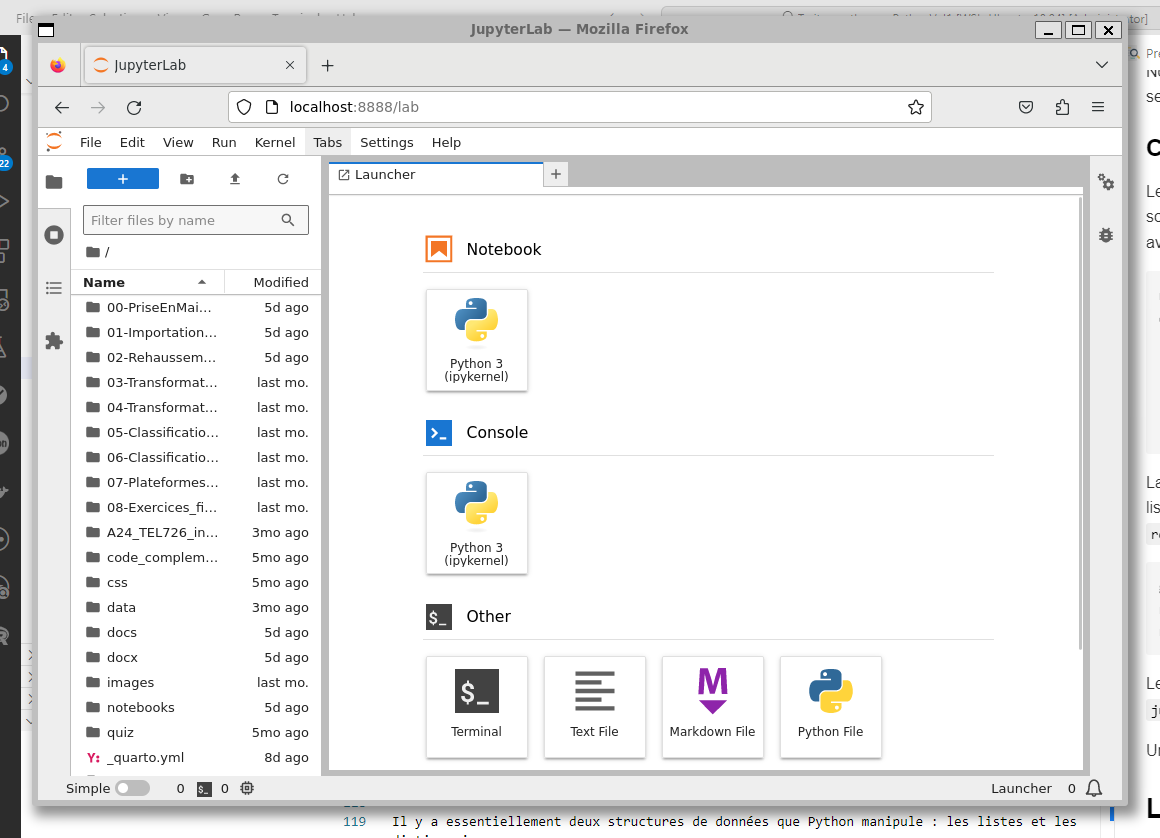
\includegraphics[width=1\linewidth,height=\textheight,keepaspectratio]{images/jupyter-accueil.png}

}

\caption[Client Jupyter Lab]{\label{fig-jupyterlab}Fenêtre principale du
serveur Jupyter Lab.}

\end{figure}%

\section{Les structures de base en
Python}\label{les-structures-de-base-en-python}

Il y a essentiellement deux structures de données que Python manipule :
les listes et les dictionnaires.

\subsection{Les listes}\label{les-listes}

Les listes sont comme des boites extensibles où vous pouvez ranger
différents types d'objets:

\begin{itemize}
\item
  Représentées par des crochets : \texttt{{[}1,\ 2,\ 3,\ "python"{]}}.
\item
  Ordonnées et modifiables (\emph{mutable}), vous pouvez récupérer une
  valeur par sa position avec \texttt{{[}{]}}.
\item
  Permettent les doublons (deux fois la même valeur).
\item
  Idéales pour stocker des collections d'éléments que vous voulez
  modifier
\end{itemize}

\subsection{Les tuples}\label{les-tuples}

Les tuples sont similaires aux listes, mais les boîtes sont scellées:

\begin{itemize}
\item
  Représentés par des parenthèses : \texttt{(1,\ 2,\ 3,\ "python")}.
\item
  Ordonnés mais non modifiables (\emph{immutable}).
\item
  Permettent les doublons.
\item
  Souvent utilisés pour stocker des données qui ne doivent pas changer
  (comme des paramètres).
\end{itemize}

\subsection{Les ensembles (Sets)}\label{les-ensembles-sets}

Les ensembles sont comme des boites magiques qui ne gardent qu'un
exemplaire de chaque objet:

\begin{itemize}
\item
  Représentés par des accolades : \texttt{\{1,\ 2,\ 3\}}.
\item
  Non ordonnés et modifiables.
\item
  N'autorisent pas les doublons.
\item
  Utiles pour éliminer les doublons et effectuer des opérations
  mathématiques sur des ensembles.
\end{itemize}

\section{Dictionnaires}\label{dictionnaires}

Les dictionnaires sont comme des boites avec des étiquettes sur chcune
d'elle :

\begin{itemize}
\item
  Représentés par des accolades avec des paires clé-valeur :
  \texttt{\{"nom":\ "Python",\ "année":\ 1991\}}.
\item
  Non ordonnés et modifiables.
\item
  Les clés doivent être uniques, mais les valeurs peuvent être
  dupliquées
\item
  Utiles pour stocker des données associatives ou pour créer des tables
  de recherche rapide
\end{itemize}

\section{Programmation objet}\label{programmation-objet}

La programmation orientée objet (POO) en Python est comme construire
avec des blocs LEGO. Chaque objet est un bloc LEGO avec ses propres
caractéristiques (attributs) et capacités (méthodes). Les classes sont
les plans pour créer ces blocs. Par exemple, une classe ``Voiture''
pourrait avoir des attributs comme ``couleur'' et ``vitesse'', et des
méthodes comme ``démarrer'' et ``accélérer''.

Python rend la POO accessible avec des fonctionnalités conviviales:

\begin{enumerate}
\def\labelenumi{\arabic{enumi}.}
\item
  \textbf{Encapsulation}: comme emballer un cadeau, elle cache les
  détails internes d'un objet.
\item
  \textbf{Héritage}: permet de créer de nouvelles classes basées sur des
  classes existantes, comme un enfant héritant des traits de ses
  parents.
\item
  \textbf{Polymorphisme}: permet à différents objets de répondre au même
  message de manière unique, comme si différents animaux répondaient
  différemment à ``fais du bruit''.
\end{enumerate}

Ces caractéristiques font de Python un excellent choix pour apprendre et
appliquer les concepts de la POO, rendant le code plus organisé et
réutilisable

\begin{tcolorbox}[colback=background_color, colframe=package_color, boxrule=0.2mm, leftrule=1mm, coltitle=black, fonttitle=\bfseries, title={
\includegraphics[width=0.3cm]{images/BlocPackage.png} \textbf{Package}}]

\textbf{Liste des \emph{packages} utilisés dans ce chapitre}

\begin{itemize}
\tightlist
\item
  Pour importer et manipuler des fichiers géographiques~:

  \begin{itemize}
  \tightlist
  \item
    \texttt{numpy} pour manipuler des données matricielles.
  \item
    \texttt{rasterio} pour importer et manipuler des données
    matricielles.
  \end{itemize}
\item
  Pour construire des cartes et des graphiques~:

  \begin{itemize}
  \tightlist
  \item
    \texttt{matplotlib} est certainement le \emph{package} le plus
    complet pour l'affichage général.
  \item
    \texttt{seaborn} pour construire des graphiques plus détaillés en
    particulier pour les statistiques.
  \end{itemize}
\end{itemize}

\end{tcolorbox}

\bookmarksetup{startatroot}

\chapter{Importation et manipulation de données
spatiales}\label{sec-chap01}

\section{Préambule}\label{pruxe9ambule}

Assurez-vous de lire ce préambule avant d'exécutez le reste du notebook.

\subsection{Objectifs}\label{objectifs}

Dans ce chapitre, nous abordons quelques formats d'images ainsi que leur
lecture. Ce chapitre est aussi disponible sous la forme d'un notebook
Python:

\href{https://colab.research.google.com/github/sfoucher/TraitementImagesPythonVol1/blob/main/notebooks/01-ImportationManipulationImages.ipynb}{\pandocbounded{
\includegraphics[keepaspectratio]{images/colab.png}}}

\begin{tcolorbox}[colback=background_color, colframe=objectif_color, boxrule=0.2mm, leftrule=1mm, coltitle=black, fonttitle=\bfseries, title={
\includegraphics[width=0.3cm]{images/BlocObjectif.png} \textbf{Objectif}}]

\textbf{Objectifs d'apprentissage visés dans ce chapitre}

À la fin de ce chapitre, vous devriez être en mesure de~:

\begin{itemize}
\tightlist
\item
  connaître les principales bibliothèques Python pour lire une image;
\item
  accéder à l'information d'une image avant de la lire;
\item
  comprendre les principaux formats pour une image
\item
  manipuler la matrice de la donnée d'une image avec numpy
\end{itemize}

\end{tcolorbox}

\subsection{Bibliothèques}\label{bibliothuxe8ques}

Les bibliothèques qui vont être explorées dans ce chapitre sont les
suivantes:

\begin{itemize}
\item
  \href{https://scipy.org/}{SciPy}
\item
  \href{https://numpy.org/}{NumPy}
\item
  \href{https://pypi.org/project/opencv-python/}{opencv-python · PyPI}
\item
  \href{https://scikit-image.org/}{scikit-image}
\item
  \href{https://rasterio.readthedocs.io/en/stable/}{Rasterio}
\item
  \href{https://docs.xarray.dev/en/stable/}{Xarray}
\item
  \href{https://corteva.github.io/rioxarray/stable/index.html}{rioxarray}
\end{itemize}

Dans l'environnement Google Colab, seul \texttt{rioxarray} et
\texttt{gdal} doivent être installés:

\begin{Shaded}
\begin{Highlighting}[]
\OperatorTok{!}\NormalTok{apt}\OperatorTok{{-}}\NormalTok{get update}
\OperatorTok{!}\NormalTok{apt}\OperatorTok{{-}}\NormalTok{get install gdal}\OperatorTok{{-}}\BuiltInTok{bin}\NormalTok{ libgdal}\OperatorTok{{-}}\NormalTok{dev}
\OperatorTok{!}\NormalTok{pip install }\OperatorTok{{-}}\NormalTok{q rioxarray}
\end{Highlighting}
\end{Shaded}

Vérifier les importations:

\begin{Shaded}
\begin{Highlighting}[]
\ImportTok{import}\NormalTok{ numpy }\ImportTok{as}\NormalTok{ np}
\ImportTok{import}\NormalTok{ rioxarray }\ImportTok{as}\NormalTok{ rxr}
\ImportTok{from}\NormalTok{ scipy }\ImportTok{import}\NormalTok{ signal}
\ImportTok{import}\NormalTok{ xarray }\ImportTok{as}\NormalTok{ xr}
\ImportTok{import}\NormalTok{ xrscipy}
\ImportTok{import}\NormalTok{ matplotlib.pyplot }\ImportTok{as}\NormalTok{ plt}
\end{Highlighting}
\end{Shaded}

\subsection{Données}\label{donnuxe9es}

Nous utilisons ces images dans ce chapitre:

\begin{Shaded}
\begin{Highlighting}[]
\ImportTok{import}\NormalTok{ gdown}

\NormalTok{gdown.download(}\StringTok{\textquotesingle{}https://drive.google.com/uc?export=download\&confirm=pbef\&id=1a6Ypg0g1Oy4AJt9XWKWfnR12NW1XhNg\_\textquotesingle{}}\NormalTok{, output}\OperatorTok{=} \StringTok{\textquotesingle{}RGBNIR\_of\_S2A.tif\textquotesingle{}}\NormalTok{)}
\NormalTok{gdown.download(}\StringTok{\textquotesingle{}https://drive.google.com/uc?export=download\&confirm=pbef\&id=1a4PQ68Ru8zBphbQ22j0sgJ4D2quw{-}Wo6\textquotesingle{}}\NormalTok{, output}\OperatorTok{=} \StringTok{\textquotesingle{}landsat7.tif\textquotesingle{}}\NormalTok{)}
\NormalTok{gdown.download(}\StringTok{\textquotesingle{}https://drive.google.com/uc?export=download\&confirm=pbef\&id=1\_zwCLN{-}x7XJcNHJCH6Z8upEdUXtVtvs1\textquotesingle{}}\NormalTok{, output}\OperatorTok{=} \StringTok{\textquotesingle{}berkeley.jpg\textquotesingle{}}\NormalTok{)}
\OperatorTok{!}\NormalTok{wget https:}\OperatorTok{//}\NormalTok{raw.githubusercontent.com}\OperatorTok{/}\NormalTok{sfoucher}\OperatorTok{/}\NormalTok{TraitementImagesPythonVol1}\OperatorTok{/}\NormalTok{refs}\OperatorTok{/}\NormalTok{heads}\OperatorTok{/}\NormalTok{main}\OperatorTok{/}\NormalTok{images}\OperatorTok{/}\NormalTok{modis}\OperatorTok{{-}}\NormalTok{aqua.PNG }\OperatorTok{{-}}\NormalTok{O modis}\OperatorTok{{-}}\NormalTok{aqua.PNG}
\end{Highlighting}
\end{Shaded}

Vérifiez que vous êtes capable de les lire:

\begin{Shaded}
\begin{Highlighting}[]
\ControlFlowTok{with}\NormalTok{ rxr.open\_rasterio(}\StringTok{\textquotesingle{}berkeley.jpg\textquotesingle{}}\NormalTok{, mask\_and\_scale}\OperatorTok{=} \VariableTok{True}\NormalTok{) }\ImportTok{as}\NormalTok{ img\_rgb:}
    \BuiltInTok{print}\NormalTok{(img\_rgb)}
\ControlFlowTok{with}\NormalTok{ rxr.open\_rasterio(}\StringTok{\textquotesingle{}RGBNIR\_of\_S2A.tif\textquotesingle{}}\NormalTok{, mask\_and\_scale}\OperatorTok{=} \VariableTok{True}\NormalTok{) }\ImportTok{as}\NormalTok{ img\_rgbnir:}
    \BuiltInTok{print}\NormalTok{(img\_rgbnir)}
\end{Highlighting}
\end{Shaded}

\section{Importation d'images}\label{importation-dimages}

La première étape avant tout traitement est d'accéder à la donnée image
pour qu'elle soit manipulée par le langage Python. L'imagerie satellite
présente certains défis notamment en raison de la taille parfois très
importante des images. Il existe maintenant certaines bibliothèques,
comme \href{https://docs.xarray.dev/en/stable/}{Xarray}, qui visent à
optimiser la lecture et l'écriture de grandes images. Il est donc
conseillé de toujours garder un oeil sur l'espace mémoire occupé par les
variables Python représentant les images. La librairie principale en
géomatique qui permettre d'importer (et d'exporter) de l'imagerie est la
librairie \href{https://gdal.org}{GDAL} qui rassemble la plupart des
formats sous forme de \emph{driver} (ou pilote en français).

Dans le domaine de la géomatique, il faut prêter attention à trois
caractéristiques principales des images:

1. \textbf{La matrice des données} elle-même qui contient les valeurs
brutes des pixels. Cette matrice sera souvent un cube à trois
dimensions. En Python, ce cube sera le plus souvent un objet de la
librairie \href{https://numpy.org/}{NumPy} (voir section).

2. \textbf{La dynamique des images} c.-à.-d le format de stockage des
valeurs individuelles (octet, entier, double, etc.). Ce format décide
principalement de la résolution radiométrique et des valeurs minimales
et maximales supportées.

3. \textbf{Le nombre de bandes} spectrales de l'image qui est souvent
supérieur à trois et peut atteindre plusieurs centaines de bandes pour
certains capteurs (notamment hyperspectraux).

4. \textbf{La métadonnée} qui va transporter l'information auxiliaire de
l'image comme les dimensions et la position de l'image, la date, etc.
Cette donnée auxiliaire prendra souvent la forme d'un dictionnaire
Python. Elle contiendra aussi l'information de géoréférence.

Les différents formats se distinguent principalement sur la manière dont
ces trois caractéristiques sont gérées.

\subsection{Formats des images}\label{formats-des-images}

Il existe de nombreux formats numériques pour la donnée de type image
parfois appelé donnée matricielle ou donnée \emph{raster}. La librairie
GDAL rassemble la plupart des formats matriciels rencontrés en
géomatique (voir
\href{https://gdal.org/en/latest/drivers/raster/index.html}{Raster
drivers --- GDAL documentation} pour une liste complète).

On peut distinguer deux grandes familles de format:

1. Les formats de type \textbf{RVB} issus de l'imagerie numérique grand
public comme
\href{https://gdal.org/en/latest/drivers/raster/jpeg.html\#raster-jpeg}{JPEG},
\href{https://gdal.org/en/latest/drivers/raster/png.html\#raster-png}{png},
etc. Ces formats ne supportent généralement que trois bandes au maximum
(rouge, vert et bleu) et des valeurs de niveaux de gris entre 0 et 255
(format dit 8 bits ou \texttt{uint8}).

2. \textbf{Les géo-formats} issus des domaines scientifiques ou
techniques comme GeoTIFF, HDF5, NetCDF, etc. qui peuvent inclure plus
que trois bandes et des dynamiques plus élevées (16 bits ou même float).

Les formats RVB restent très utilisés en Python notamment par les
bibliothèques dites de vision par ordinateur (\emph{Computer Vision})
comme OpenCV et sickit-image ainsi que les grandes bibliothèques en
apprentissage profond (PyTorch, Tensorflow).

\begin{tcolorbox}[colback=background_color, colframe=package_color, boxrule=0.2mm, leftrule=1mm, coltitle=black, fonttitle=\bfseries, title={
\includegraphics[width=0.3cm]{images/BlocPackage.png} \textbf{Package}}]

\textbf{Installation de gdal dans un système Linux}

\begin{itemize}
\tightlist
\item
  Pour installer GDAL~:
\end{itemize}

\begin{verbatim}
!apt-get update
!apt-get install gdal-bin libgdal-dev
\end{verbatim}

\end{tcolorbox}

\subsubsection{Formats de type RVB}\label{formats-de-type-rvb}

Les premiers formats pour de l'imagerie à une bande (monochrome) et à
trois bandes (image couleur rouge-vert-bleu) sont issus du domaine des
sciences de l'ordinateur. On trouvera, entre autres, les formats pbm,
png et jpeg. Ces formats supportent peu de métadonnées et sont placées
dans un entête (\emph{header}) très limité. Cependant, ils restent très
populaires dans le domaine de la vision par ordinateur et sont très
utilisés en apprentissage profond en particulier. Pour la lecture des
images RVB, on peut utiliser les bibliothèques Rasterio,
\href{https://he-arc.github.io/livre-python/pillow/index.html}{PIL} ou
\href{https://docs.opencv.org/4.10.0/index.html}{OpenCV}.

\paragraph{Lecture avec la librairie
PIL}\label{lecture-avec-la-librairie-pil}

La librairie PIL retourne un objet de type \texttt{PngImageFile},
l'affichage de l'image se fait directement dans la cellule de sortie.

\begin{Shaded}
\begin{Highlighting}[]
\ImportTok{from}\NormalTok{ PIL }\ImportTok{import}\NormalTok{ Image}
\NormalTok{img }\OperatorTok{=}\NormalTok{ Image.}\BuiltInTok{open}\NormalTok{(}\StringTok{\textquotesingle{}modis{-}aqua.PNG\textquotesingle{}}\NormalTok{)}
\NormalTok{img}
\end{Highlighting}
\end{Shaded}

\pandocbounded{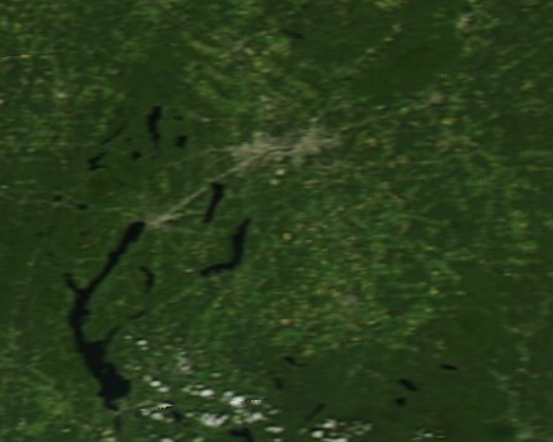
\includegraphics[keepaspectratio]{01-ImportationManipulationImages_files/figure-pdf/cell-6-output-1.png}}

\paragraph{Lecture avec la librairie
OpenCV}\label{lecture-avec-la-librairie-opencv}

La librairie \href{https://docs.opencv.org/4.10.0/index.html}{OpenCV}
est aussi très populaire en vision par ordinateur. La fonction
\texttt{imread} donne directement un objet de type NumPy en sortie.

\begin{Shaded}
\begin{Highlighting}[]
\ImportTok{import}\NormalTok{ cv2}
\NormalTok{img }\OperatorTok{=}\NormalTok{ cv2.imread(}\StringTok{\textquotesingle{}modis{-}aqua.PNG\textquotesingle{}}\NormalTok{)}
\NormalTok{img}
\end{Highlighting}
\end{Shaded}

\begin{verbatim}
array([[[17, 50, 33],
        [15, 49, 31],
        [14, 48, 30],
        ...,
        [23, 56, 36],
        [23, 55, 36],
        [22, 55, 36]],

       [[18, 51, 34],
        [16, 50, 32],
        [15, 49, 32],
        ...,
        [27, 59, 40],
        [28, 60, 41],
        [27, 60, 41]],

       [[18, 53, 35],
        [18, 52, 34],
        [18, 51, 34],
        ...,
        [31, 64, 44],
        [34, 66, 47],
        [33, 65, 46]],

       ...,

       [[34, 74, 48],
        [35, 73, 48],
        [34, 70, 46],
        ...,
        [41, 74, 54],
        [41, 73, 54],
        [41, 73, 54]],

       [[36, 76, 50],
        [36, 74, 49],
        [35, 71, 47],
        ...,
        [37, 70, 51],
        [38, 71, 51],
        [38, 71, 51]],

       [[36, 76, 50],
        [35, 73, 48],
        [33, 69, 45],
        ...,
        [31, 63, 44],
        [33, 65, 46],
        [33, 66, 46]]], dtype=uint8)
\end{verbatim}

\paragraph{Lecture avec la librairie
RasterIO}\label{lecture-avec-la-librairie-rasterio}

Rien ne nous empêche de lire une image de format RVB avec
\href{https://rasterio.readthedocs.io/en/stable/}{RasterIO} comme décrit
dans ci-dessous. Vous noterez cependant les avertissements concernant
l'absence de géoréférence pour ce type d'image.

\begin{Shaded}
\begin{Highlighting}[]
\ImportTok{import}\NormalTok{ rasterio}
\NormalTok{img}\OperatorTok{=}\NormalTok{ rasterio.}\BuiltInTok{open}\NormalTok{(}\StringTok{\textquotesingle{}modis{-}aqua.PNG\textquotesingle{}}\NormalTok{)}
\NormalTok{img}
\end{Highlighting}
\end{Shaded}

\begin{verbatim}
<open DatasetReader name='modis-aqua.PNG' mode='r'>
\end{verbatim}

\subsubsection{Le format GeoTiff}\label{le-format-geotiff}

Le format GeoTIFF est une extension du format TIFF (Tagged Image File
Format) qui permet d'incorporer des métadonnées géospatiales directement
dans un fichier image. Développé initialement par Dr.~Niles Ritter au
Jet Propulsion Laboratory de la
\href{https://www.earthdata.nasa.gov/esdis/esco/standards-and-practices/geotiff}{NASA}
dans les années 1990, GeoTIFF est devenu un standard de facto pour le
stockage et l'échange d'images géoréférencées dans les domaines de la
télédétection et des systèmes d'information géographique (SIG). Ce
format supporte plus que trois bandes aussi longtemps que ces bandes
sont de même dimension.

Le format GeoTIFF est très utilisé et est largement supporté par les
bibliothèques et logiciels géospatiaux, notamment
\href{https://gdal.org}{GDAL} (\emph{Geospatial Data Abstraction
Library}), qui offre des capacités de lecture et d'écriture pour ce
format. Cette compatibilité étendue a contribué à son adoption
généralisée dans la communauté géospatiale.

\paragraph{Standardisation par l'OGC}\label{standardisation-par-logc}

Le standard GeoTIFF proposé par l'Open Geospatial Consortium (OGC) en
2019 formalise et étend les spécifications originales du format GeoTIFF,
offrant une norme robuste pour l'échange d'images géoréférencées. Cette
standardisation, connue sous le nom d'OGC GeoTIFF 1.1 (2019), apporte
plusieurs améliorations et clarifications importantes.

\subsubsection{Le format COG}\label{le-format-cog}

Une innovation récente dans l'écosystème GeoTIFF est le format
\emph{Cloud Optimized GeoTIFF} (\href{http://cogeo.org/}{COG}), conçu
pour faciliter l'utilisation de fichiers GeoTIFF hébergés sur des
serveurs web HTTP. Le COG permet aux utilisateurs et aux logiciels
d'accéder à des parties spécifiques du fichier sans avoir à le
télécharger entièrement, ce qui est particulièrement utile pour les
applications basées sur l'infonuagique.

\subsection{Métadonnées des images}\label{muxe9tadonnuxe9es-des-images}

La manière la plus directe d'accéder à la métadonnée d'une image est
d'utiliser les commandes
\href{https://rasterio.readthedocs.io/en/stable/cli.html\#info}{\texttt{rio\ info}}
de la librairie Rasterio ou \texttt{gdalinfo} de la librairie
\texttt{gdal}. Le résultat est imprimé dans la sortie standard ou sous
forme d'un dictionnaire Python.

\begin{Shaded}
\begin{Highlighting}[]
\OperatorTok{!}\NormalTok{gdalinfo RGBNIR\_of\_S2A.tif}
\end{Highlighting}
\end{Shaded}

\begin{verbatim}
Warning 1: TIFFReadDirectory:Sum of Photometric type-related color channels and ExtraSamples doesn't match SamplesPerPixel. Defining non-color channels as ExtraSamples.
Driver: GTiff/GeoTIFF
Files: RGBNIR_of_S2A.tif
       RGBNIR_of_S2A.tif.aux.xml
Size is 2074, 1926
Coordinate System is:
PROJCS["WGS 84 / UTM zone 18N",
    GEOGCS["WGS 84",
        DATUM["WGS_1984",
            SPHEROID["WGS 84",6378137,298.257223563,
                AUTHORITY["EPSG","7030"]],
            AUTHORITY["EPSG","6326"]],
        PRIMEM["Greenwich",0,
            AUTHORITY["EPSG","8901"]],
        UNIT["degree",0.0174532925199433,
            AUTHORITY["EPSG","9122"]],
        AUTHORITY["EPSG","4326"]],
    PROJECTION["Transverse_Mercator"],
    PARAMETER["latitude_of_origin",0],
    PARAMETER["central_meridian",-75],
    PARAMETER["scale_factor",0.9996],
    PARAMETER["false_easting",500000],
    PARAMETER["false_northing",0],
    UNIT["metre",1,
        AUTHORITY["EPSG","9001"]],
    AXIS["Easting",EAST],
    AXIS["Northing",NORTH],
    AUTHORITY["EPSG","32618"]]
Origin = (731780.000000000000000,5040800.000000000000000)
Pixel Size = (10.000000000000000,-10.000000000000000)
Metadata:
  AREA_OR_POINT=Area
  TIFFTAG_IMAGEDESCRIPTION=subset_RGBNIR_of_S2A_MSIL2A_20240625T153941_N0510_R011_T18TYR_20240625T221903
  TIFFTAG_RESOLUTIONUNIT=1 (unitless)
  TIFFTAG_XRESOLUTION=1
  TIFFTAG_YRESOLUTION=1
Image Structure Metadata:
  INTERLEAVE=BAND
Corner Coordinates:
Upper Left  (  731780.000, 5040800.000) ( 72d 2' 3.11"W, 45d28'55.98"N)
Lower Left  (  731780.000, 5021540.000) ( 72d 2'35.69"W, 45d18'32.70"N)
Upper Right (  752520.000, 5040800.000) ( 71d46' 9.19"W, 45d28'30.08"N)
Lower Right (  752520.000, 5021540.000) ( 71d46'44.67"W, 45d18' 6.95"N)
Center      (  742150.000, 5031170.000) ( 71d54'23.16"W, 45d23'31.71"N)
Band 1 Block=2074x1926 Type=UInt16, ColorInterp=Gray
  Min=86.000 Max=15104.000 
  Minimum=86.000, Maximum=15104.000, Mean=1426.625, StdDev=306.564
  Metadata:
    STATISTICS_MAXIMUM=15104
    STATISTICS_MEAN=1426.6252674912
    STATISTICS_MINIMUM=86
    STATISTICS_STDDEV=306.56427126942
    STATISTICS_VALID_PERCENT=100
Band 2 Block=2074x1926 Type=UInt16, ColorInterp=Undefined
  Min=1139.000 Max=14352.000 
  Minimum=1139.000, Maximum=14352.000, Mean=1669.605, StdDev=310.919
  Metadata:
    STATISTICS_MAXIMUM=14352
    STATISTICS_MEAN=1669.6050060032
    STATISTICS_MINIMUM=1139
    STATISTICS_STDDEV=310.91935787639
    STATISTICS_VALID_PERCENT=100
Band 3 Block=2074x1926 Type=UInt16, ColorInterp=Undefined
  Min=706.000 Max=15280.000 
  Minimum=706.000, Maximum=15280.000, Mean=1471.392, StdDev=385.447
  Metadata:
    STATISTICS_MAXIMUM=15280
    STATISTICS_MEAN=1471.3923473736
    STATISTICS_MINIMUM=706
    STATISTICS_STDDEV=385.44654593014
    STATISTICS_VALID_PERCENT=100
Band 4 Block=2074x1926 Type=UInt16, ColorInterp=Undefined
  Min=1067.000 Max=15642.000 
  Minimum=1067.000, Maximum=15642.000, Mean=4393.945, StdDev=1037.934
  Metadata:
    STATISTICS_MAXIMUM=15642
    STATISTICS_MEAN=4393.94485025
    STATISTICS_MINIMUM=1067
    STATISTICS_STDDEV=1037.933939728
    STATISTICS_VALID_PERCENT=100
\end{verbatim}

Le plus simple est d'utiliser la fonction \texttt{rio\ info}:

\begin{Shaded}
\begin{Highlighting}[]
\OperatorTok{!}\NormalTok{rio info RGBNIR\_of\_S2A.tif }\OperatorTok{{-}{-}}\NormalTok{indent }\DecValTok{2} \OperatorTok{{-}{-}}\NormalTok{verbose}
\end{Highlighting}
\end{Shaded}

\section{Manipulation des images}\label{manipulation-des-images}

\subsection{Manipulation de la matrice de
pixels}\label{manipulation-de-la-matrice-de-pixels}

La donnée brute de l'image est généralement contenue dans un cube
matricielle à trois dimensions (deux dimensions spatiales et une
dimension spectrale). Comme exposé précédemment, la librairie dite
\emph{``fondationnelle''} pour la manipulation de matrices en Python est
\href{https://numpy.org/}{NumPy}. Cette librairie contient un nombre
très important de fonctionnalités couvrant l'algèbre linéaire, les
statistiques, etc.; elle constitue la fondation de nombreuses
bibliothèques en traitement numérique (voir
(figure~\ref{fig-naturenumpy1}))

\begin{figure}

\centering{

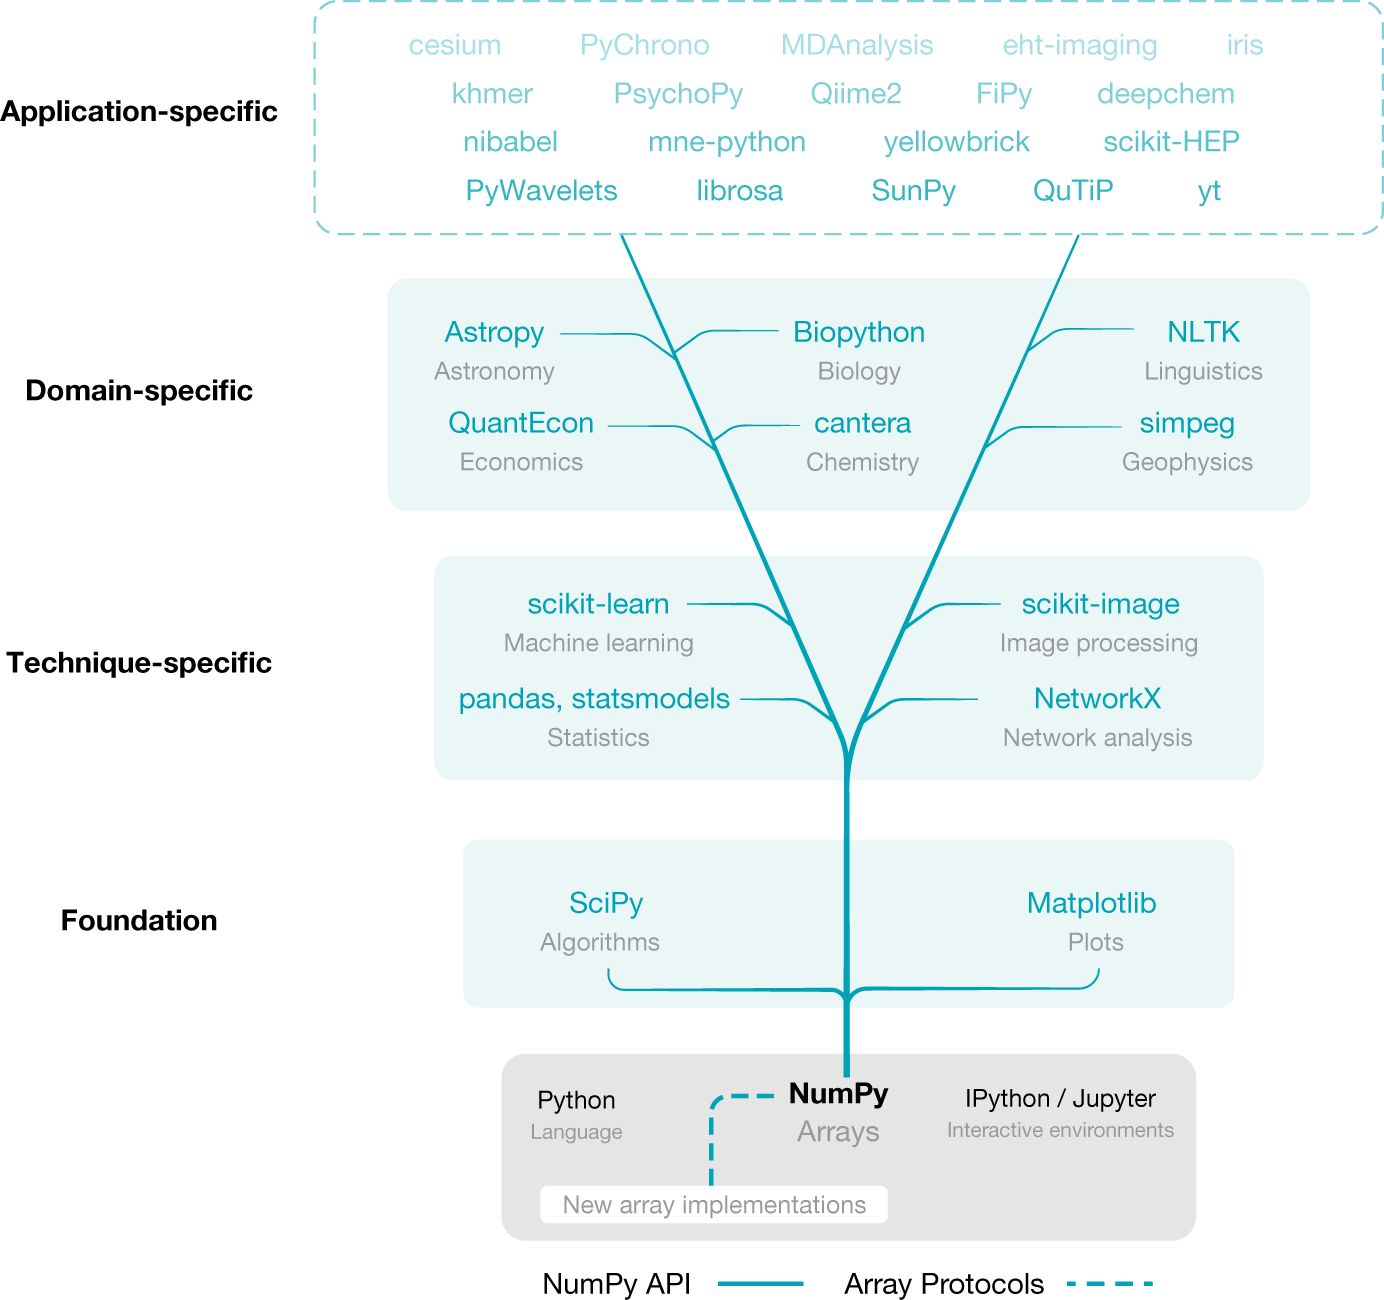
\includegraphics[width=1\linewidth,height=\textheight,keepaspectratio]{images/41586_2020_2649_Fig2_HTML.png}

}

\caption{\label{fig-naturenumpy1}La librairie NumPy est le fondement de
nombreuses bibliothèques scientifiques (d'après (Harris 2020)).}

\end{figure}%

\subsection{Information de base}\label{information-de-base}

Les deux informations de base à afficher sur une matrice sont 1) les
dimensions de la matrice et 2) le format de stockage (le type). Pour
cela, on peut utiliser le code ci-dessous, dont le résultat nous informe
que la matrice a trois dimensions et une taille de
\texttt{(442,\ 553,\ 3)} et un type \texttt{uint8} qui représente 1
octet (8 bit). Par conséquent, la matrice a \texttt{442} lignes,
\texttt{553} colonnes et \texttt{3} canaux ou bandes. Il faut prêter une
attention particulière aux valeurs minimales et maximales tolérées par
le type de la donnée comme indiqué dans le (tableau~\ref{tbl-numpytype})
(voir aussi
\href{https://numpy.org/doc/stable/user/basics.types.html}{Data types
--- NumPy v2.1 Manual}).

\begin{Shaded}
\begin{Highlighting}[]
\ImportTok{import}\NormalTok{ cv2}
\NormalTok{img }\OperatorTok{=}\NormalTok{ cv2.imread(}\StringTok{\textquotesingle{}modis{-}aqua.PNG\textquotesingle{}}\NormalTok{)}
\BuiltInTok{print}\NormalTok{(}\StringTok{\textquotesingle{}Nombre de dimensions: \textquotesingle{}}\NormalTok{,img.ndim)}
\BuiltInTok{print}\NormalTok{(}\StringTok{\textquotesingle{}Dimensions de la matrice: \textquotesingle{}}\NormalTok{,img.shape)}
\BuiltInTok{print}\NormalTok{(}\StringTok{\textquotesingle{}Type de la donnée: \textquotesingle{}}\NormalTok{,img.dtype)}
\end{Highlighting}
\end{Shaded}

\begin{verbatim}
Nombre de dimensions:  3
Dimensions de la matrice:  (442, 553, 3)
Type de la donnée:  uint8
\end{verbatim}

\begin{longtable}[]{@{}llrrr@{}}

\caption{\label{tbl-numpytype}Type de données de NumPy}

\tabularnewline

\toprule\noalign{}
dtype & Nom & Taille (bits) & Min & Max \\
\midrule\noalign{}
\endhead
\bottomrule\noalign{}
\endlastfoot
uint8 & char & 8 & 0 & 255 \\
int8 & signed char & 8 & -127 & 128 \\
uint16 & unsigned short & 16 & 0 & -32768 \\
int16 & short & 16 & 0 & 655355 \\

\end{longtable}

\subsection{Découpage et indexation de la
matrice}\label{duxe9coupage-et-indexation-de-la-matrice}

L'indexation et le découpage (\emph{slicing}) des matrices dans NumPy
sont des techniques essentielles pour manipuler efficacement les données
multidimensionnelles en Python, offrant une syntaxe puissante et
flexible pour accéder et modifier des sous-ensembles spécifiques
d'éléments dans les tableaux (voir figure~\ref{fig-naturenumpy2}).
Indexer une matrice consiste à accéder à une valeur dans la matrice pour
une position particulière, la syntaxe générale est
\texttt{matrice{[}ligne,\ colonne,\ bande{]}} et est similaire à la
manipulation des
\href{https://docs.python.org/fr/3/tutorial/introduction.html\#lists}{listes}
en Python. Les indices commencent à \texttt{0} et se termine à la
\texttt{taille-1} de l'axe considéré.

\begin{figure}

\centering{

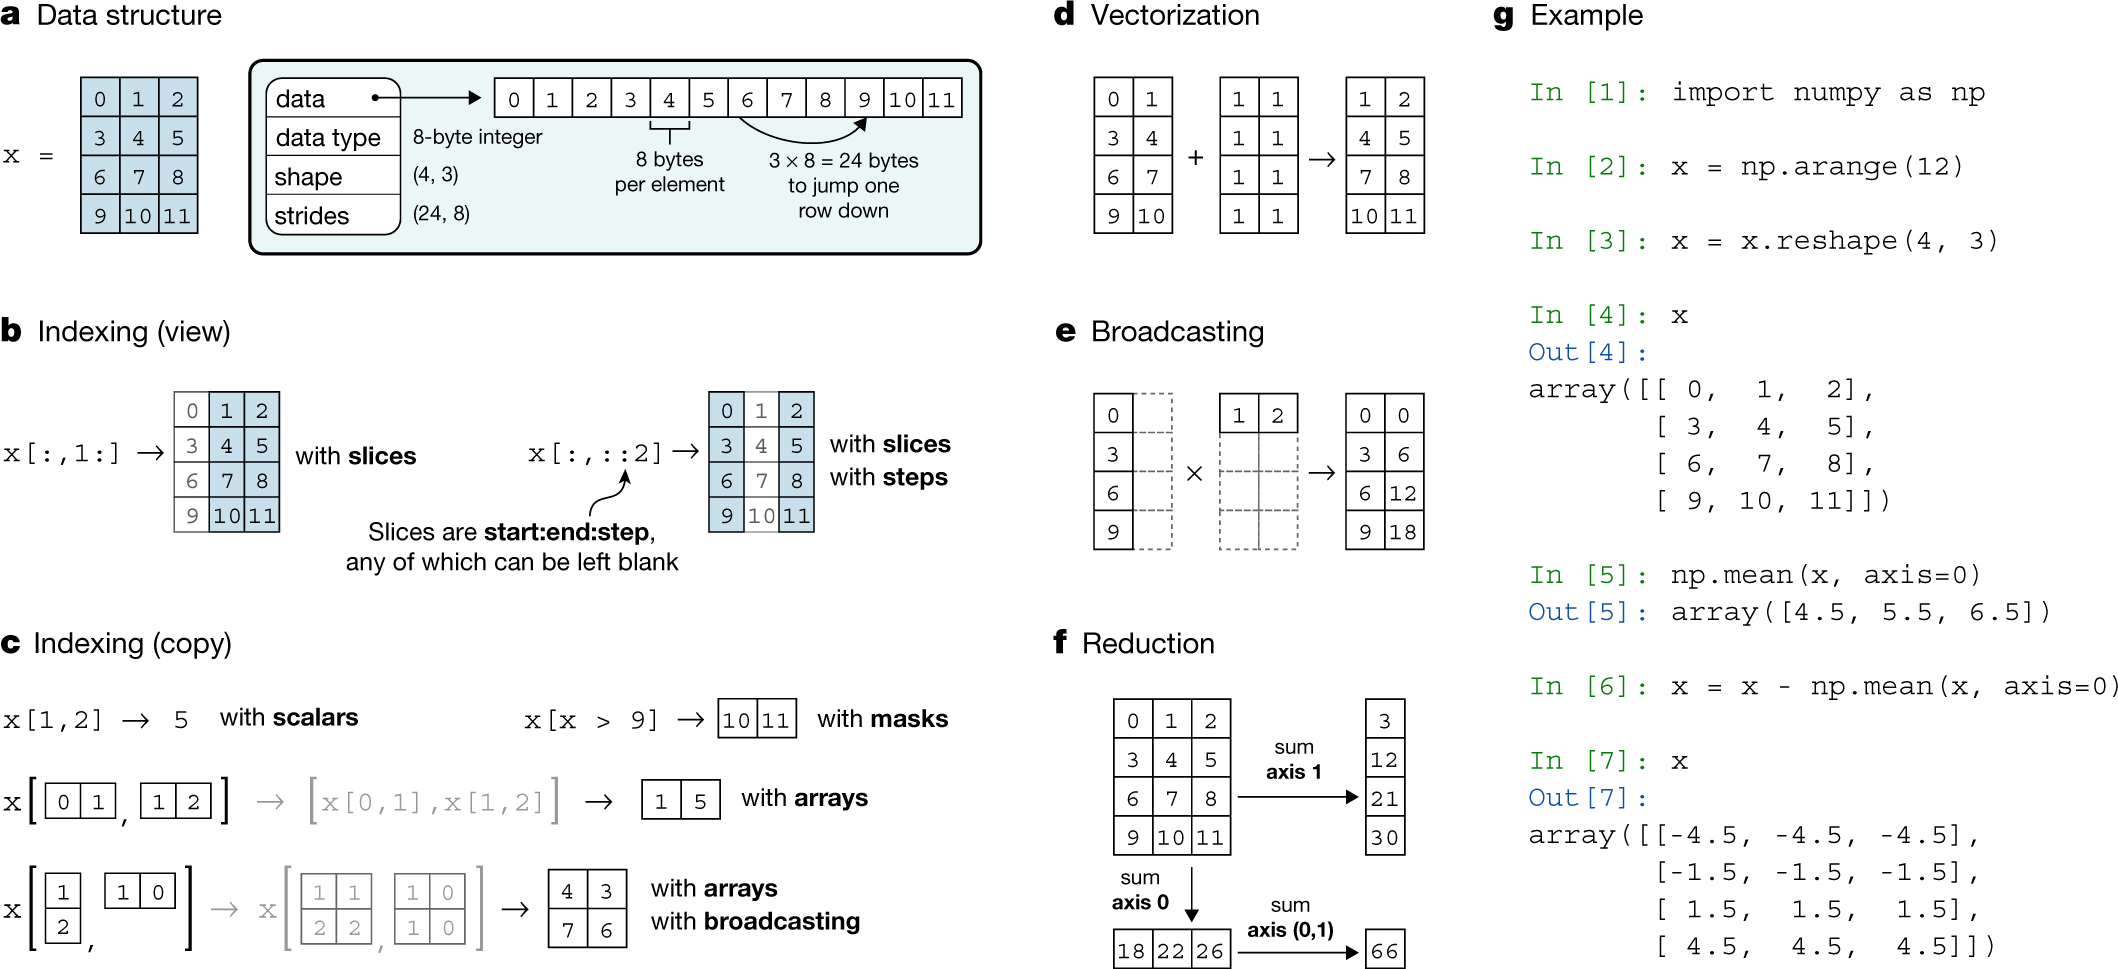
\includegraphics[width=1\linewidth,height=\textheight,keepaspectratio]{images/41586_2020_2649_Fig1_HTML.png}

}

\caption{\label{fig-naturenumpy2}Vue d'ensemble des opérations de base
des matrices avec NumPy}

\end{figure}%

Le découpage (ou \emph{slicing} en anglais) consiste à produire une
nouvelle matrice qui est un sous-ensemble de la matrice d'origine. Un
découpage se fait avec le symbole `:', la syntaxe générale pour définir
un découpage est \texttt{{[}début:fin:pas{]}}. Si on ne spécifie pas
\texttt{début} ou \texttt{fin} alors les valeurs 0 ou
\texttt{dimension-1} sont considérées implicitement. Quelques exemples:
* choisir un pixel en particulier avec toutes les bandes:
\texttt{matrice{[}1,1,:{]}} * choisir la colonne 2:
\texttt{matrice{[}:,2,:{]}}

La syntaxe de base pour le découpage (\emph{slicing}) des tableaux NumPy
repose sur l'utilisation des deux-points (\texttt{:}) à l'intérieur des
crochets d'indexation. Cette notation permet de sélectionner des plages
d'éléments de manière concise et intuitive. La structure générale du
découpage est \texttt{matrice{[}start:stop:step{]}}, où : 1.
\texttt{start} représente l'index de départ (inclus) 2. \texttt{stop}
indique l'index de fin (exclu) 3. \texttt{step} définit l'intervalle
entre chaque élément sélectionné

Si l'un de ces paramètres est omis, NumPy utilise des valeurs par défaut
: 0 pour \texttt{start}, la taille du tableau pour \texttt{stop}, et 1
pour \texttt{step}. Par exemple, pour un tableau unidimensionnel
\texttt{array}, on peut extraire les éléments du deuxième au quatrième
avec \texttt{array{[}1:4{]}}. Pour sélectionner tous les éléments à
partir du troisième, on utiliserait \texttt{array{[}2:{]}}. Cette
syntaxe s'applique également aux tableaux multidimensionnels, où chaque
dimension est séparée par une virgule. Ainsi, pour une matrice 2D m,
\texttt{m{[}0:2,\ 1:3{]}} sélectionnerait une sous-matrice 2x2 composée
des deux premières lignes et des deuxième et troisième colonnes.
L'indexation négative est également supportée, permettant de compter à
partir de la fin du tableau. Par exemple, \texttt{a{[}-3:{]}}
sélectionnerait les trois derniers éléments d'un tableau.

\begin{Shaded}
\begin{Highlighting}[]
\ImportTok{import}\NormalTok{ cv2}
\NormalTok{img }\OperatorTok{=}\NormalTok{ cv2.imread(}\StringTok{\textquotesingle{}modis{-}aqua.PNG\textquotesingle{}}\NormalTok{)}
\NormalTok{img\_col }\OperatorTok{=}\NormalTok{ img[:,}\DecValTok{1}\NormalTok{,:]}
\BuiltInTok{print}\NormalTok{(}\StringTok{\textquotesingle{}Nombre de dimensions: \textquotesingle{}}\NormalTok{,img\_col.ndim)}
\BuiltInTok{print}\NormalTok{(}\StringTok{\textquotesingle{}Dimensions de la matrice: \textquotesingle{}}\NormalTok{,img\_col.shape)}
\end{Highlighting}
\end{Shaded}

\begin{verbatim}
Nombre de dimensions:  2
Dimensions de la matrice:  (442, 3)
\end{verbatim}

\begin{tcolorbox}[colback=background_color, colframe=allerloin_color, boxrule=0.2mm, leftrule=1mm, coltitle=black, fonttitle=\bfseries, title={
\includegraphics[width=0.3cm]{images/BlocAllerPlusLoin.png} \textbf{Aller plus loin}}]

\textbf{Une vue versus une copie}

Avec NumPy, les manipulations peuvent créer des vues ou des copies. Une
vue est une simple représentation de la même donnée originale alors
qu'une copie est un nouvel espace mémoire.

Par défaut, un découpage créé une vue.

On peut vérifier si l'espace mémoire est partagé avec
\texttt{np.shares\_memory(arr,\ slice\_arr)}.

On peut toujours forcer une copie avec la méthode \texttt{copy()}

\end{tcolorbox}

\subsubsection{Masquage}\label{masquage}

L'utilisation d'un masque est un outil important en traitement d'image
car la plupart des images de télédétection contiennent des pixels non
valides qu'il faut exclure des traitements (ce que l'on appelle le
\emph{no data} en Anglais). Il y a plusieurs raison possibles pour la
présence de pixels non valides:

\begin{enumerate}
\def\labelenumi{\arabic{enumi}.}
\item
  L'image est projetée dans une grille cartographique et certaines
  zones, généralement situées en dehors de l'empreinte au sol du
  capteur, sont à exclure.
\item
  La présence de nuages que l'on veut exclure.
\item
  La présence de pixels erronés dus à des problèmes de capteurs.
\item
  La présence de valeurs non numériques (\emph{not a number} ou
  \texttt{nan})
\end{enumerate}

La librairie NumPy fournit des mécanismes pour exclure automatiquement
certaines valeurs.

\subsection{Changement de projection cartographique (à
venir)}\label{changement-de-projection-cartographique-uxe0-venir}

\section{Données en géoscience}\label{donnuxe9es-en-guxe9oscience}

Les données en géoscience contiennent beaucoup de métadonnées et peuvent
être composées de différentes variables avec différentes unités,
résolution, etc. Ces données sont aussi souvent étiquetées avec des
dates sur certains axes, des coordonnées géographiques, des identifiants
d'expériences, etc. Par conséquent, utiliser seulement des matrices est
souvent incomplet (Hoyer et Hamman 2017).

Calibration, unités, données manquantes, données éparses.

\subsection{xarray}\label{xarray}

\href{https://docs.xarray.dev/en/latest/getting-started-guide/why-xarray.html}{Xarray}
est une puissante bibliothèque Python qui améliore les matrices
multidimensionnelles de type numpy en y ajoutant des étiquettes, des
dimensions, des coordonnées et des attributs. Elle fournit deux
structures de données principales : \texttt{DataArray} (un tableau
étiqueté à n dimensions) et \texttt{Dataset} (une base de données de
tableaux multidimensionnels en mémoire).

Les caractéristiques principales sont les suivantes:

\begin{itemize}
\item
  Opérations sur les dimensions nommées au lieu des numéros d'axe
\item
  Sélection et opérations basées sur les étiquettes
\item
  Diffusion automatique de tableaux basée sur les noms de dimensions
\item
  Alignement de type base de données avec des étiquettes de coordonnées
\item
  Suivi des métadonnées grâce à des dictionnaires Python
\end{itemize}

\subsubsection{Avantages}\label{avantages}

La bibliothèque réduit considérablement la complexité du code et
améliore la lisibilité du code pour les applications de calcul
scientifique dans divers domaines, notamment la physique, l'astronomie,
les géosciences, la bio-informatique, l'ingénierie, la finance et
l'apprentissage profond. Elle s'intègre de manière transparente avec
NumPy et pandas tout en restant compatible avec l'écosystème Python au
sens large.

\subsubsection{DataArray}\label{dataarray}

Un tableau multidimensionnel étiqueté avec des propriétés clées :

\begin{itemize}
\item
  \texttt{valeurs} : Les données réelles du tableau
\item
  \texttt{dims} : Dimensions nommées (par exemple, « x », « y », « z »)
\item
  \texttt{coords} : Dictionnaire de tableaux étiquetant chaque point
\item
  \texttt{attrs} : Stockage de métadonnées arbitraires
\item
  \texttt{name} : Identifiant facultatif
\end{itemize}

\subsubsection{Dataset}\label{dataset}

Un conteneur de type dictionnaire de \texttt{DataArrays} avec des
dimensions alignées, contenant :

\begin{itemize}
\item
  \texttt{dims} : Dictionnaire de correspondance entre les noms des
  dimensions et les longueurs
\item
  \texttt{data\_vars} : Dictionnaire des variables du DataArray
\item
  \texttt{coords} : Dictionnaire des variables de coordonnées
\item
  \texttt{attrs} : Stockage des métadonnées
\end{itemize}

Les principales différences sont les suivantes :

\begin{itemize}
\item
  \texttt{DataArray} contient un seul tableau avec des étiquettes
\item
  Le \texttt{Dataset} contient plusieurs DataArrays alignés.
\end{itemize}

Ces trois structures prennent en charge les opérations de type
dictionnaire et les calculs de coordination tout en conservant les
métadonnées.

\begin{figure}

\centering{

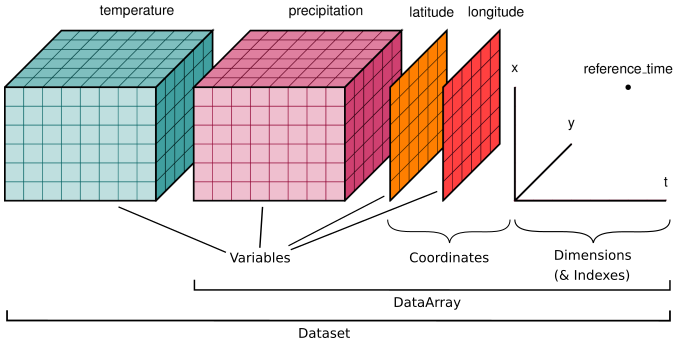
\includegraphics[width=0.8\linewidth,height=\textheight,keepaspectratio]{images/xarray-dataset-diagram.png}

}

\caption{\label{fig-xarray}Organisation d'un Dataset dans xarray}

\end{figure}%

\bookmarksetup{startatroot}

\chapter{Réhaussement et visualisation d'images}\label{sec-chap02}

Assurez-vous de lire ce préambule avant d'exécutez le reste du notebook.

\section{Préambule}\label{pruxe9ambule-1}

\subsection{Objectifs}\label{objectifs-1}

Dans ce chapitre, nous abordons quelques techniques de réhaussement et
de visualisation d'images. Ce chapitre est aussi disponible sous la
forme d'un notebook Python:

\href{https://colab.research.google.com/github/sfoucher/TraitementImagesPythonVol1/blob/main/notebooks/02-RehaussementVisualisationImages.ipynb}{\pandocbounded{
\includegraphics[keepaspectratio]{images/colab.png}}}

\begin{tcolorbox}[colback=background_color, colframe=objectif_color, boxrule=0.2mm, leftrule=1mm, coltitle=black, fonttitle=\bfseries, title={
\includegraphics[width=0.3cm]{images/BlocObjectif.png} \textbf{Objectif}}]

\textbf{Objectifs d'apprentissage visés dans ce chapitre}

À la fin de ce chapitre, vous devriez être en mesure de~:

\begin{itemize}
\tightlist
\item
  exploiter les statistiques d'une image pour améliorer la
  visualisation;
\item
  calculer les histogrammes de valeurs;
\item
  appliquer une transformation linéaire ou non linéaire pour améliorer
  une visualisation;
\item
  comprendre le principe des composés colorés;
\end{itemize}

\end{tcolorbox}

\subsection{}\label{section}

\subsection{Bibliothèques}\label{bibliothuxe8ques-1}

Les bibliothèques qui vont être explorées dans ce chapitre sont les
suivantes:

\begin{itemize}
\item
  \href{https://scipy.org/}{SciPy}
\item
  \href{https://numpy.org/}{NumPy}
\item
  \href{https://pypi.org/project/opencv-python/}{opencv-python · PyPI}
\item
  \href{https://scikit-image.org/}{scikit-image}
\item
  \href{https://rasterio.readthedocs.io/en/stable/}{Rasterio}
\item
  \href{https://docs.xarray.dev/en/stable/}{Xarray}
\item
  \href{https://corteva.github.io/rioxarray/stable/index.html}{rioxarray}
\end{itemize}

Dans l'environnement Google Colab, seul \texttt{rioxarray} et GDAL
doivent être installés:

\begin{Shaded}
\begin{Highlighting}[]
\OperatorTok{\%\%}\NormalTok{capture}
\OperatorTok{!}\NormalTok{apt}\OperatorTok{{-}}\NormalTok{get update}
\OperatorTok{!}\NormalTok{apt}\OperatorTok{{-}}\NormalTok{get install gdal}\OperatorTok{{-}}\BuiltInTok{bin}\NormalTok{ libgdal}\OperatorTok{{-}}\NormalTok{dev}
\end{Highlighting}
\end{Shaded}

Dans l'environnement \href{https://colab.research.google.com/}{Google
Colab}, il convient de s'assurer que les librairies sont installées:

\begin{Shaded}
\begin{Highlighting}[]
\OperatorTok{\%\%}\NormalTok{capture}
\OperatorTok{!}\NormalTok{pip install }\OperatorTok{{-}}\NormalTok{qU matplotlib rioxarray xrscipy scikit}\OperatorTok{{-}}\NormalTok{image}
\end{Highlighting}
\end{Shaded}

Vérifier les importations:

\begin{Shaded}
\begin{Highlighting}[]
\ImportTok{import}\NormalTok{ numpy }\ImportTok{as}\NormalTok{ np}
\ImportTok{import}\NormalTok{ rioxarray }\ImportTok{as}\NormalTok{ rxr}
\ImportTok{from}\NormalTok{ scipy }\ImportTok{import}\NormalTok{ signal}
\ImportTok{import}\NormalTok{ xarray }\ImportTok{as}\NormalTok{ xr}
\ImportTok{import}\NormalTok{ xrscipy}
\ImportTok{import}\NormalTok{ matplotlib.pyplot }\ImportTok{as}\NormalTok{ plt}
\end{Highlighting}
\end{Shaded}

\subsection{Données}\label{donnuxe9es-1}

Nous utiliserons les images suivantes dans ce chapitre:

\begin{Shaded}
\begin{Highlighting}[]
\OperatorTok{\%\%}\NormalTok{capture}
\ImportTok{import}\NormalTok{ gdown}

\NormalTok{gdown.download(}\StringTok{\textquotesingle{}https://drive.google.com/uc?export=download\&confirm=pbef\&id=1a6Ypg0g1Oy4AJt9XWKWfnR12NW1XhNg\_\textquotesingle{}}\NormalTok{, output}\OperatorTok{=} \StringTok{\textquotesingle{}RGBNIR\_of\_S2A.tif\textquotesingle{}}\NormalTok{)}
\NormalTok{gdown.download(}\StringTok{\textquotesingle{}https://drive.google.com/uc?export=download\&confirm=pbef\&id=1a6O3L\_abOfU7h94K22At8qtBuLMGErwo\textquotesingle{}}\NormalTok{, output}\OperatorTok{=} \StringTok{\textquotesingle{}sentinel2.tif\textquotesingle{}}\NormalTok{)}
\NormalTok{gdown.download(}\StringTok{\textquotesingle{}https://drive.google.com/uc?export=download\&confirm=pbef\&id=1\_zwCLN{-}x7XJcNHJCH6Z8upEdUXtVtvs1\textquotesingle{}}\NormalTok{, output}\OperatorTok{=} \StringTok{\textquotesingle{}berkeley.jpg\textquotesingle{}}\NormalTok{)}
\NormalTok{gdown.download(}\StringTok{\textquotesingle{}https://drive.google.com/uc?export=download\&confirm=pbef\&id=1dM6IVqjba6GHwTLmI7CpX8GP2z5txUq6\textquotesingle{}}\NormalTok{, output}\OperatorTok{=} \StringTok{\textquotesingle{}SAR.tif\textquotesingle{}}\NormalTok{)}
\end{Highlighting}
\end{Shaded}

Vérifiez que vous êtes capable de les lire :

\begin{Shaded}
\begin{Highlighting}[]
\ControlFlowTok{with}\NormalTok{ rxr.open\_rasterio(}\StringTok{\textquotesingle{}berkeley.jpg\textquotesingle{}}\NormalTok{, mask\_and\_scale}\OperatorTok{=} \VariableTok{True}\NormalTok{) }\ImportTok{as}\NormalTok{ img\_rgb:}
    \BuiltInTok{print}\NormalTok{(img\_rgb)}
\ControlFlowTok{with}\NormalTok{ rxr.open\_rasterio(}\StringTok{\textquotesingle{}sentinel2.tif\textquotesingle{}}\NormalTok{, mask\_and\_scale}\OperatorTok{=} \VariableTok{True}\NormalTok{) }\ImportTok{as}\NormalTok{ img\_s2:}
    \BuiltInTok{print}\NormalTok{(img\_s2)}
\ControlFlowTok{with}\NormalTok{ rxr.open\_rasterio(}\StringTok{\textquotesingle{}RGBNIR\_of\_S2A.tif\textquotesingle{}}\NormalTok{, mask\_and\_scale}\OperatorTok{=} \VariableTok{True}\NormalTok{) }\ImportTok{as}\NormalTok{ img\_rgbnir:}
    \BuiltInTok{print}\NormalTok{(img\_rgbnir)}
\ControlFlowTok{with}\NormalTok{ rxr.open\_rasterio(}\StringTok{\textquotesingle{}SAR.tif\textquotesingle{}}\NormalTok{, mask\_and\_scale}\OperatorTok{=} \VariableTok{True}\NormalTok{) }\ImportTok{as}\NormalTok{ img\_SAR:}
    \BuiltInTok{print}\NormalTok{(img\_SAR)}
\end{Highlighting}
\end{Shaded}

\section{Visualisation en Python}\label{visualisation-en-python}

ID'emblée, il faut mentionner que Python n'est pas vraiment fait pour
visualiser de la donnée de grande taille, le niveau d'interactivité est
aussi assez limité. Pour une visualisation interactives, il est plutôt
conseillé d'utiliser un outil comme \href{https://qgis.org/}{QGIS}.
Néanmoins, il est possible de visualiser de petites images avec la
librairie \href{https://matplotlib.org/stable/}{\texttt{matplotlib}} qui
est la librairie principale de visualisation en Python. Cette librairie
est extrêmement riche et versatile, nous ne présenterons que les bases
nécessaires pour démarrer. Le lecteur désirant aller plus loin pourra
consulter les nombreux tutoriels disponibles comme
\href{https://matplotlib.org/stable/tutorials/index.html}{celui-ci}.

La fonction de base pour créer une figure est \texttt{subplots}, la
largeur et la hauteur en pouces de la figure peuvent être contrôlées via
le paramètre \texttt{figsize}:

\begin{Shaded}
\begin{Highlighting}[]
\ImportTok{import}\NormalTok{ matplotlib.pyplot }\ImportTok{as}\NormalTok{ plt}
\NormalTok{fig, ax}\OperatorTok{=}\NormalTok{ plt.subplots(figsize}\OperatorTok{=}\NormalTok{(}\DecValTok{5}\NormalTok{, }\DecValTok{4}\NormalTok{))}
\NormalTok{plt.show()}
\end{Highlighting}
\end{Shaded}

\pandocbounded{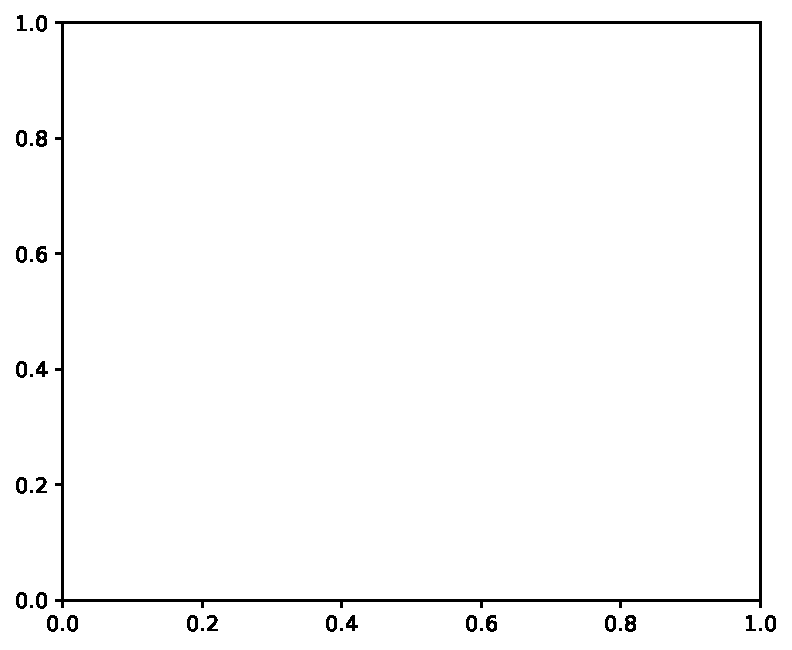
\includegraphics[keepaspectratio]{02-RehaussementVisualisationImages_files/figure-pdf/cell-8-output-1.pdf}}

Pour l'affichage des images, la fonction \texttt{imshow} permet
d'afficher une matrice 2D à une dimension en format \emph{float} ou une
matrice RVB avec 3 bandes. Il est important que les dimensions de la
matrice soient dans l'ordre hauteur, largeur et bande.

\begin{Shaded}
\begin{Highlighting}[]
\ImportTok{import}\NormalTok{ matplotlib.pyplot }\ImportTok{as}\NormalTok{ plt}
\NormalTok{fig, ax}\OperatorTok{=}\NormalTok{ plt.subplots(figsize}\OperatorTok{=}\NormalTok{(}\DecValTok{6}\NormalTok{, }\DecValTok{5}\NormalTok{))}
\NormalTok{plt.imshow(img\_rgbnir[}\DecValTok{0}\NormalTok{].data)}
\NormalTok{plt.show()}
\end{Highlighting}
\end{Shaded}

\pandocbounded{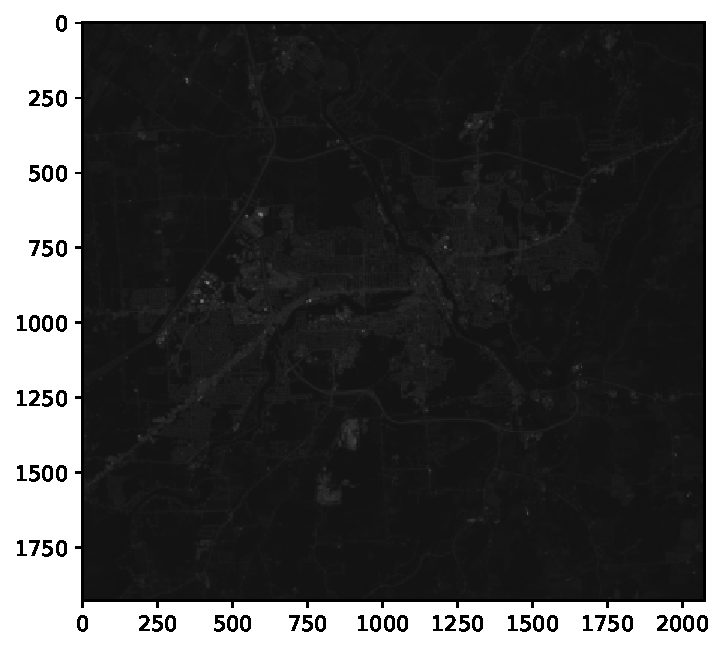
\includegraphics[keepaspectratio]{02-RehaussementVisualisationImages_files/figure-pdf/cell-9-output-1.pdf}}

Pour un affichage à trois bandes, les valeurs seront ramenées sur une
échelle de 0 à 1, il est donc nécessaire de normaliser les valeurs avant
l'affichage:

\begin{Shaded}
\begin{Highlighting}[]
\ImportTok{import}\NormalTok{ matplotlib.pyplot }\ImportTok{as}\NormalTok{ plt}
\NormalTok{fig, ax}\OperatorTok{=}\NormalTok{ plt.subplots(figsize}\OperatorTok{=}\NormalTok{(}\DecValTok{6}\NormalTok{, }\DecValTok{5}\NormalTok{))}
\NormalTok{plt.imshow(img\_rgbnir.data.transpose(}\DecValTok{1}\NormalTok{,}\DecValTok{2}\NormalTok{,}\DecValTok{0}\NormalTok{)}\OperatorTok{/}\FloatTok{2500.0}\NormalTok{)}
\NormalTok{plt.show()}
\end{Highlighting}
\end{Shaded}

\pandocbounded{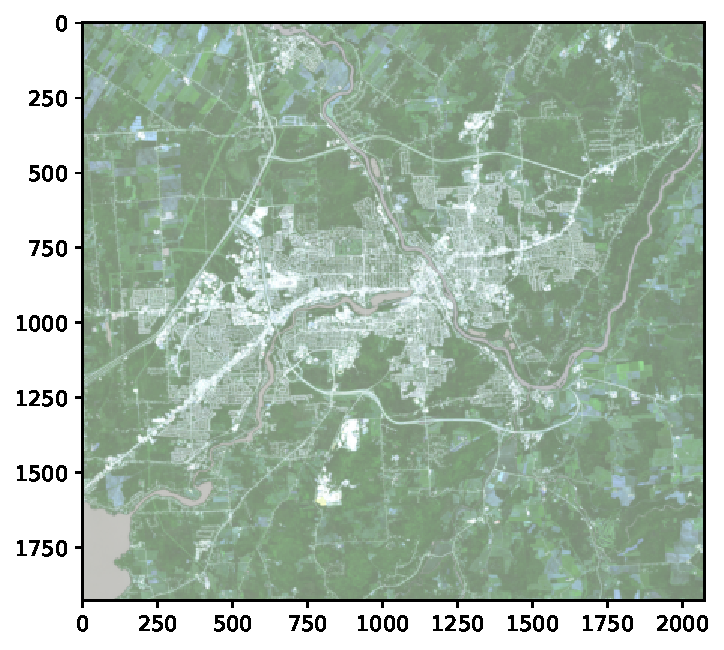
\includegraphics[keepaspectratio]{02-RehaussementVisualisationImages_files/figure-pdf/cell-10-output-1.pdf}}

On remarquera les valeurs des axes \texttt{x} et \texttt{y} avec une
origine en haut à gauche. Ceci est un référentiel purement matriciel
(lignes et colonnes); autrement dit, il n'y a pas ici de géoréférence.
Pour pallier à cette limitation, les librairies \texttt{rasterio} et
\texttt{xarray} proposent une extension de la fonction \texttt{imshow}
permettant d'afficher les coordonnées cartographiques ainsi qu'un
contrôle la dynamique de l'image:

\begin{Shaded}
\begin{Highlighting}[]
\ImportTok{import}\NormalTok{ rioxarray }\ImportTok{as}\NormalTok{ rxr}
\NormalTok{fig, ax}\OperatorTok{=}\NormalTok{ plt.subplots(figsize}\OperatorTok{=}\NormalTok{(}\DecValTok{6}\NormalTok{, }\DecValTok{5}\NormalTok{))}
\NormalTok{img\_rgbnir.sel(band}\OperatorTok{=}\NormalTok{[}\DecValTok{1}\NormalTok{,}\DecValTok{2}\NormalTok{,}\DecValTok{3}\NormalTok{]).plot.imshow(vmin}\OperatorTok{=}\DecValTok{86}\NormalTok{, vmax}\OperatorTok{=}\DecValTok{5000}\NormalTok{)}
\NormalTok{ax.set\_title(}\StringTok{\textquotesingle{}Imshow avec rioxarray\textquotesingle{}}\NormalTok{)}
\NormalTok{plt.show()}
\end{Highlighting}
\end{Shaded}

\pandocbounded{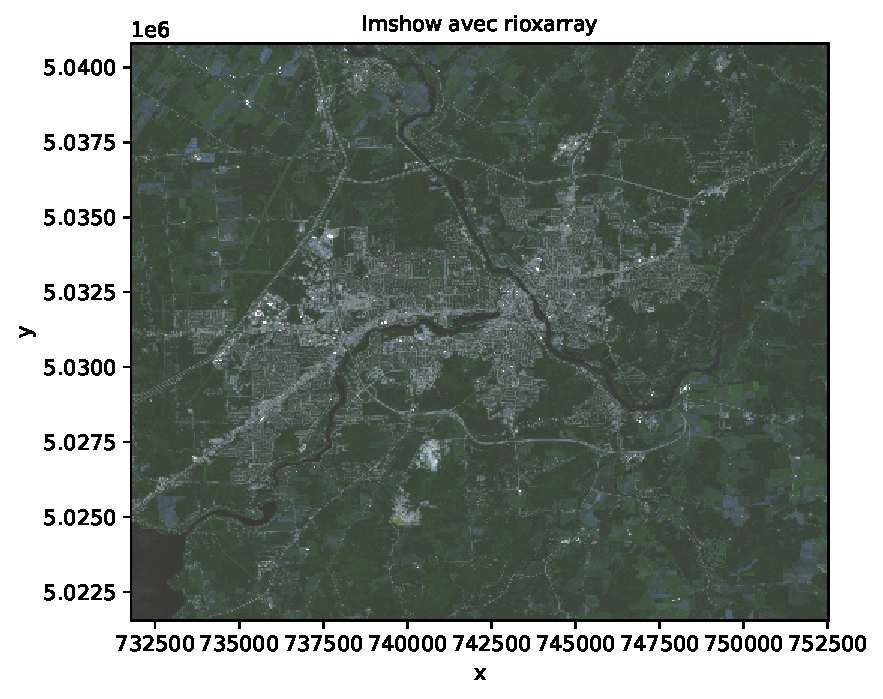
\includegraphics[keepaspectratio]{02-RehaussementVisualisationImages_files/figure-pdf/cell-11-output-1.pdf}}

\section{Réhaussements visuels}\label{ruxe9haussements-visuels}

Le réhaussement visuel d'une image vise principalement à améliorer la
qualité visuelle d'une image en améliorant le contraste, la dynamique ou
la texture d'une image. De manière générale, ce réhaussement ne modifie
pas la donnée d'origine mais il est appliquée dynamiquement à
l'affichage pour des fins d'inspection visuelle. Le réhaussement
nécessite généralement une connaissance des caractéristiques
statistiques d'une image. Ces statistiques sont ensuite exploitées pour
appliquer diverses transformations linéaires ou non linéaires.

\subsection{Statistiques d'une image}\label{statistiques-dune-image}

On peut considérer un ensemble de statistique pour chacune des bandes
d'une image:

\begin{itemize}
\item
  valeurs minimales et maximales
\item
  valeurs moyennes,
\item
  Quartiles (1er quartile, médiane et 3ième quartile), quantiles et
  percentiles.
\item
  écart-type, et coefficients d'asymétrie (\emph{skewness}) et
  d'applatissement (\emph{kurtosis})
\end{itemize}

Ces statistiques doivent être calculées pour chaque bande d'une image
multispectrale.

En ligne de commande, \texttt{gdalinfo} permet d'interroger rapidement
un fichier image pour connaitre ces statistiques univariées de base:

\begin{Shaded}
\begin{Highlighting}[]
\OperatorTok{!}\NormalTok{gdalinfo }\OperatorTok{{-}}\NormalTok{stats landsat7.tif}
\end{Highlighting}
\end{Shaded}

\begin{verbatim}
Driver: GTiff/GeoTIFF
Files: landsat7.tif
       landsat7.tif.aux.xml
Size is 2181, 1917
Coordinate System is:
PROJCS["WGS 84 / Pseudo-Mercator",
    GEOGCS["WGS 84",
        DATUM["WGS_1984",
            SPHEROID["WGS 84",6378137,298.257223563,
                AUTHORITY["EPSG","7030"]],
            AUTHORITY["EPSG","6326"]],
        PRIMEM["Greenwich",0,
            AUTHORITY["EPSG","8901"]],
        UNIT["degree",0.0174532925199433,
            AUTHORITY["EPSG","9122"]],
        AUTHORITY["EPSG","4326"]],
    PROJECTION["Mercator_1SP"],
    PARAMETER["central_meridian",0],
    PARAMETER["scale_factor",1],
    PARAMETER["false_easting",0],
    PARAMETER["false_northing",0],
    UNIT["metre",1,
        AUTHORITY["EPSG","9001"]],
    AXIS["X",EAST],
    AXIS["Y",NORTH],
    EXTENSION["PROJ4","+proj=merc +a=6378137 +b=6378137 +lat_ts=0.0 +lon_0=0.0 +x_0=0.0 +y_0=0 +k=1.0 +units=m +nadgrids=@null +wktext +no_defs"],
    AUTHORITY["EPSG","3857"]]
Origin = (-13651650.000000000000000,4576290.000000000000000)
Pixel Size = (30.000000000000000,-30.000000000000000)
Metadata:
  AREA_OR_POINT=Area
  OVR_RESAMPLING_ALG=NEAREST
  TIFFTAG_RESOLUTIONUNIT=1 (unitless)
  TIFFTAG_XRESOLUTION=1
  TIFFTAG_YRESOLUTION=1
Image Structure Metadata:
  COMPRESSION=DEFLATE
  INTERLEAVE=PIXEL
Corner Coordinates:
Upper Left  (-13651650.000, 4576290.000) (122d38' 5.49"W, 37d58'40.08"N)
Lower Left  (-13651650.000, 4518780.000) (122d38' 5.49"W, 37d34'10.00"N)
Upper Right (-13586220.000, 4576290.000) (122d 2'49.53"W, 37d58'40.08"N)
Lower Right (-13586220.000, 4518780.000) (122d 2'49.53"W, 37d34'10.00"N)
Center      (-13618935.000, 4547535.000) (122d20'27.51"W, 37d46'26.05"N)
Band 1 Block=512x512 Type=Byte, ColorInterp=Red
  Min=19.000 Max=233.000 
  Minimum=19.000, Maximum=233.000, Mean=98.433, StdDev=21.164
  NoData Value=0
  Overviews: 1091x959, 546x480
  Metadata:
    STATISTICS_MAXIMUM=233
    STATISTICS_MEAN=98.433096940153
    STATISTICS_MINIMUM=19
    STATISTICS_STDDEV=21.164021026458
Band 2 Block=512x512 Type=Byte, ColorInterp=Green
  Min=19.000 Max=178.000 
  Minimum=19.000, Maximum=178.000, Mean=55.068, StdDev=22.204
  NoData Value=0
  Overviews: 1091x959, 546x480
  Metadata:
    STATISTICS_MAXIMUM=178
    STATISTICS_MEAN=55.067787534804
    STATISTICS_MINIMUM=19
    STATISTICS_STDDEV=22.203571974581
Band 3 Block=512x512 Type=Byte, ColorInterp=Blue
  Min=19.000 Max=187.000 
  Minimum=19.000, Maximum=187.000, Mean=43.341, StdDev=20.330
  NoData Value=0
  Overviews: 1091x959, 546x480
  Metadata:
    STATISTICS_MAXIMUM=187
    STATISTICS_MEAN=43.340507443056
    STATISTICS_MINIMUM=19
    STATISTICS_STDDEV=20.32987736339
\end{verbatim}

Les librairies de base comme \texttt{rasterio} et \texttt{xarray}
produisent facilement un sommaire des statistiques de base avec la
fonction
\href{https://rasterio.readthedocs.io/en/stable/api/rasterio.io.html\#rasterio.io.BufferedDatasetWriter.stats}{stats}:

\begin{Shaded}
\begin{Highlighting}[]
\ImportTok{import}\NormalTok{ rasterio }\ImportTok{as}\NormalTok{ rio}
\ImportTok{import}\NormalTok{ numpy }\ImportTok{as}\NormalTok{ np}
\ControlFlowTok{with}\NormalTok{ rio.}\BuiltInTok{open}\NormalTok{(}\StringTok{\textquotesingle{}landsat7.tif\textquotesingle{}}\NormalTok{) }\ImportTok{as}\NormalTok{ src:}
\NormalTok{    stats}\OperatorTok{=}\NormalTok{ src.stats()}
    \BuiltInTok{print}\NormalTok{(stats)}
\end{Highlighting}
\end{Shaded}

La librairie \texttt{xarray} donne accès à des fonctionnalités plus
sophistiquées comme le calcul des quantiles:

\begin{Shaded}
\begin{Highlighting}[]
\ImportTok{import}\NormalTok{ rioxarray }\ImportTok{as}\NormalTok{ riox}
\ControlFlowTok{with}\NormalTok{ riox.open\_rasterio(}\StringTok{\textquotesingle{}landsat7.tif\textquotesingle{}}\NormalTok{, masked}\OperatorTok{=} \VariableTok{True}\NormalTok{) }\ImportTok{as}\NormalTok{ src:}
    \BuiltInTok{print}\NormalTok{(src)}
\NormalTok{quantiles }\OperatorTok{=}\NormalTok{ src.quantile(dim}\OperatorTok{=}\NormalTok{[}\StringTok{\textquotesingle{}x\textquotesingle{}}\NormalTok{,}\StringTok{\textquotesingle{}y\textquotesingle{}}\NormalTok{], q}\OperatorTok{=}\NormalTok{[}\FloatTok{.025}\NormalTok{,}\FloatTok{.25}\NormalTok{,}\FloatTok{.5}\NormalTok{,}\FloatTok{.75}\NormalTok{,}\FloatTok{.975}\NormalTok{])}
\NormalTok{quantiles}
\end{Highlighting}
\end{Shaded}

\begin{verbatim}
<xarray.DataArray (band: 3, y: 1917, x: 2181)> Size: 50MB
[12542931 values with dtype=float32]
Coordinates:
  * band         (band) int64 24B 1 2 3
  * x            (x) float64 17kB -1.365e+07 -1.365e+07 ... -1.359e+07
  * y            (y) float64 15kB 4.576e+06 4.576e+06 ... 4.519e+06 4.519e+06
    spatial_ref  int64 8B 0
Attributes:
    AREA_OR_POINT:           Area
    OVR_RESAMPLING_ALG:      NEAREST
    TIFFTAG_RESOLUTIONUNIT:  1 (unitless)
    TIFFTAG_XRESOLUTION:     1
    TIFFTAG_YRESOLUTION:     1
    STATISTICS_MAXIMUM:      233
    STATISTICS_MEAN:         98.433096940153
    STATISTICS_MINIMUM:      19
    STATISTICS_STDDEV:       21.164021026458
    scale_factor:            1.0
    add_offset:              0.0
\end{verbatim}

\begin{verbatim}
<xarray.DataArray (quantile: 5, band: 3)> Size: 120B
array([[ 54.,  19.,  19.],
       [ 85.,  38.,  27.],
       [ 99.,  54.,  38.],
       [111.,  69.,  57.],
       [140., 102.,  89.]])
Coordinates:
  * band      (band) int64 24B 1 2 3
  * quantile  (quantile) float64 40B 0.025 0.25 0.5 0.75 0.975
\end{verbatim}

\subsubsection{Calcul de l'histogramme}\label{calcul-de-lhistogramme}

Le calcul d'un histogramme pour une image (une bande) permet d'avoir une
vue plus détaillée de la répartition des valeurs radiométriques. Le
calcul d'un histogramme nécessite minimalement de faire le choix du
nombre de barre ( \emph{bins} ou de la largeur ). Un \emph{bin} est un
intervalle de valeurs pour lequel on peut calculer le nombre de valeurs
observées dans l'image. La fonction de base pour ce type de calcul est
la fonction \texttt{numpy.histogram()}:

\begin{Shaded}
\begin{Highlighting}[]
\ImportTok{import}\NormalTok{ numpy }\ImportTok{as}\NormalTok{ np}
\NormalTok{array }\OperatorTok{=}\NormalTok{ np.random.randint(}\DecValTok{0}\NormalTok{,}\DecValTok{10}\NormalTok{,}\DecValTok{100}\NormalTok{) }\CommentTok{\# 100 valeurs aléatoires entre 0 et 10}
\NormalTok{hist, bin\_limites }\OperatorTok{=}\NormalTok{ np.histogram(array, density}\OperatorTok{=}\VariableTok{True}\NormalTok{)}
\BuiltInTok{print}\NormalTok{(}\StringTok{\textquotesingle{}valeurs :\textquotesingle{}}\NormalTok{,hist)}
\BuiltInTok{print}\NormalTok{(}\StringTok{\textquotesingle{};imites :\textquotesingle{}}\NormalTok{,bin\_limites)}
\end{Highlighting}
\end{Shaded}

\begin{verbatim}
valeurs : [0.13333333 0.07777778 0.14444444 0.06666667 0.14444444 0.12222222
 0.14444444 0.11111111 0.1        0.06666667]
;imites : [0.  0.9 1.8 2.7 3.6 4.5 5.4 6.3 7.2 8.1 9. ]
\end{verbatim}

Le calcul se fait avec 10 intervalles par défaut.

\begin{Shaded}
\begin{Highlighting}[]
\NormalTok{fig, ax}\OperatorTok{=}\NormalTok{ plt.subplots(figsize}\OperatorTok{=}\NormalTok{(}\DecValTok{5}\NormalTok{, }\DecValTok{4}\NormalTok{))}
\NormalTok{plt.bar(bin\_limites[:}\OperatorTok{{-}}\DecValTok{1}\NormalTok{],hist)}
\NormalTok{plt.show()}
\end{Highlighting}
\end{Shaded}

\pandocbounded{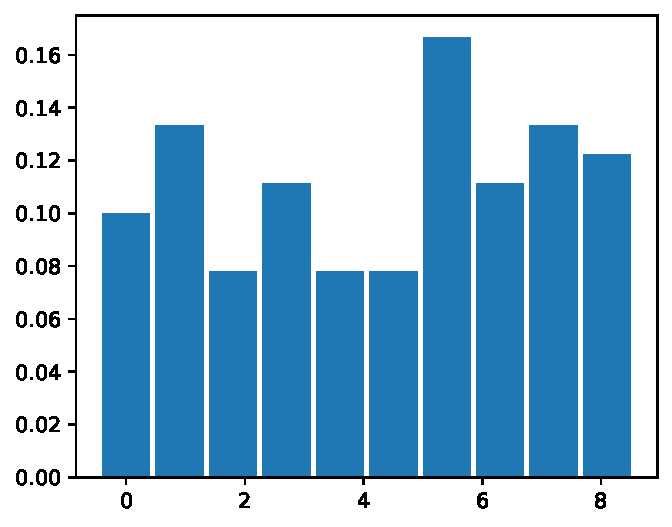
\includegraphics[keepaspectratio]{02-RehaussementVisualisationImages_files/figure-pdf/cell-16-output-1.pdf}}

Pour des besoins de visualisation, le calcul des valeurs extrêmes de
l'histogramme peut aussi se faire via les quantiles comme discutés
auparavant.

\paragraph{Visualisation des
histogrammes}\label{visualisation-des-histogrammes}

La librarie \texttt{rasterio} est probablement l'outil le plus simples
pour visualiser rapidement des histogrammes sur une image
multi-spectrale:

\begin{Shaded}
\begin{Highlighting}[]
\ImportTok{import}\NormalTok{ rasterio }\ImportTok{as}\NormalTok{ rio}
\ImportTok{from}\NormalTok{ rasterio.plot }\ImportTok{import}\NormalTok{ show\_hist}
\ControlFlowTok{with}\NormalTok{ rio.}\BuiltInTok{open}\NormalTok{(}\StringTok{\textquotesingle{}RGBNIR\_of\_S2A.tif\textquotesingle{}}\NormalTok{) }\ImportTok{as}\NormalTok{ src:}
\NormalTok{  show\_hist(src, bins}\OperatorTok{=}\DecValTok{50}\NormalTok{, lw}\OperatorTok{=}\FloatTok{0.0}\NormalTok{, stacked}\OperatorTok{=}\VariableTok{False}\NormalTok{, alpha}\OperatorTok{=}\FloatTok{0.3}\NormalTok{,histtype}\OperatorTok{=}\StringTok{\textquotesingle{}stepfilled\textquotesingle{}}\NormalTok{, title}\OperatorTok{=}\StringTok{"Histogram"}\NormalTok{)}
\end{Highlighting}
\end{Shaded}

\pandocbounded{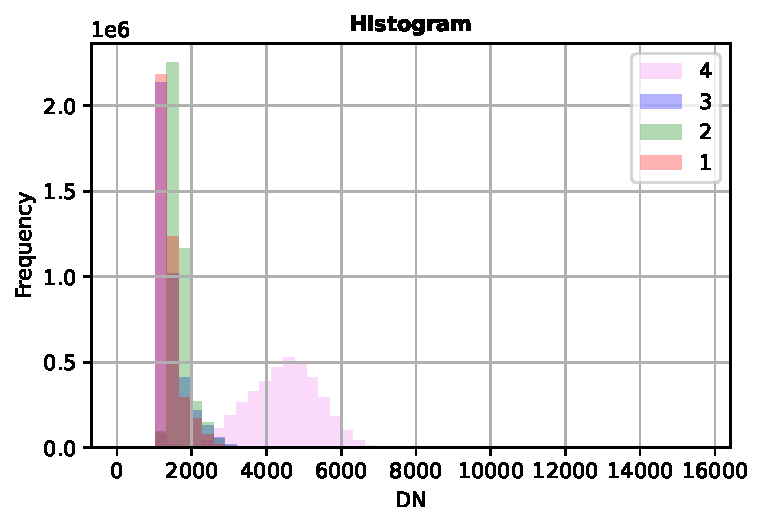
\includegraphics[keepaspectratio]{02-RehaussementVisualisationImages_files/figure-pdf/cell-17-output-1.pdf}}

\subsection{Réhaussements
linéaires}\label{ruxe9haussements-linuxe9aires}

Le réhaussement linéaire (\emph{linear stretch}) d'une image est la
forme la plus simple de réhaussement, elle consiste à 1) optimiser les
valeurs des pixels d'une image afin de maximiser la dynamique
disponibles à l'affichage, ou 2) à changer le format de stockage des
valeurs (de 8 bits à 16 bits):

\begin{equation}\phantomsection\label{eq-rehauss-lin}{ \text{nouvelle valeur d'un pixel} = \frac{\text{valeur d'un pixel} - min_0}{max_0 - min_0}\times (max_1 - min_1)+min_1}\end{equation}

Par cette opération, on passe de la dynamique de départ
(\(max_0 - min_0\)) vers la dynamique cible (\(max_1 - min_1\)). Bien
que cette opération semble triviale, il est important d'être conscient
des trois contraintes suivantes:

\begin{enumerate}
\def\labelenumi{\arabic{enumi}.}
\tightlist
\item
  \textbf{Faire attention à la dynamique cible}, ainsi, pour sauvegarder
  une image en format 8 bit, on utilisera alors \(max_1=255\) et
  \(min_1=0\).
\end{enumerate}

2. \textbf{Préservation de la valeur de no data} : il faut faire
attention à la valeur \(min_1\) dans le cas d'une valeur présente pour
\emph{no\_data}. Par exemple, si \emph{no\_data=0} alors il faut
s'assurer que \(min_1>0\).

3. \textbf{Précision du calcul} : si possible réaliser la division
ci-dessus en format \emph{float}

\subsubsection{Cas des histogrammes
asymétriques}\label{cas-des-histogrammes-asymuxe9triques}

Dans certains cas, la distribution de valeurs est très asymétrique et
présente une longue queue avec des valeurs extrêmes élevées (à droite ou
à gauche de l'histogramme). Le cas des images SAR est particulièrement
représentatif de ce type de données. En effet, celles-ci peuvent
présenter une distribution de valeurs de type exponentiel. Il est alors
préférable d'utiliser des
\href{https://fr.wikipedia.org/wiki/Centile}{percentiles} au préalable
afin d'explorer la forme de l'histogramme et la distribution des
valeurs:

\begin{Shaded}
\begin{Highlighting}[]
\NormalTok{NO\_DATA\_FLOAT}\OperatorTok{=} \OperatorTok{{-}}\FloatTok{999.0}
\CommentTok{\# on prend tous les pixels de la première bande}
\NormalTok{values }\OperatorTok{=}\NormalTok{ img\_SAR[}\DecValTok{0}\NormalTok{].values.flatten().astype(}\BuiltInTok{float}\NormalTok{)}
\CommentTok{\# on exclut les valeurs invalides}
\NormalTok{values }\OperatorTok{=}\NormalTok{ values[}\OperatorTok{\textasciitilde{}}\NormalTok{np.isnan(values)]}
\CommentTok{\# on exclut le no data}
\NormalTok{values }\OperatorTok{=}\NormalTok{ values[values}\OperatorTok{!=}\NormalTok{NO\_DATA\_FLOAT]}
\CommentTok{\# calcul des percentiles}
\NormalTok{percentiles\_position}\OperatorTok{=}\NormalTok{ (}\DecValTok{0}\NormalTok{,}\FloatTok{0.1}\NormalTok{,}\DecValTok{1}\NormalTok{,}\DecValTok{2}\NormalTok{,}\DecValTok{50}\NormalTok{,}\DecValTok{98}\NormalTok{,}\DecValTok{99}\NormalTok{,}\FloatTok{99.9}\NormalTok{,}\DecValTok{100}\NormalTok{)}
\NormalTok{percentiles}\OperatorTok{=} \BuiltInTok{dict}\NormalTok{(}\BuiltInTok{zip}\NormalTok{(percentiles\_position, np.percentile(values, percentiles\_position)))}
\BuiltInTok{print}\NormalTok{(percentiles)}
\end{Highlighting}
\end{Shaded}

\begin{verbatim}
{0: np.float64(8.172580237442162e-06), 0.1: np.float64(1.588739885482937e-05), 1: np.float64(8.657756850880105e-05), 2: np.float64(0.00018846066552214325), 50: np.float64(0.012372820172458887), 98: np.float64(0.1719470709562302), 99: np.float64(0.27963151514529694), 99.9: np.float64(1.5235805057287233), 100: np.float64(483.223876953125)}
\end{verbatim}

On constate que la valeur médiane (\texttt{0.012}) est très faible, ce
qui signifie que 50\% des valeurs sont inférieures à cette valeur alors
que la valeur maximale (\texttt{483}) est 10 000 fois plus élevée! Une
manière de visualiser cette distribution de valeurs est d'utiliser
\href{https://matplotlib.org/stable/api/_as_gen/matplotlib.pyplot.boxplot.html}{\texttt{boxplot}}
et
\href{https://matplotlib.org/stable/api/_as_gen/matplotlib.pyplot.violinplot.html}{\texttt{violinplot}}
de la librairie \texttt{matplotlib}:

\begin{Shaded}
\begin{Highlighting}[]
\NormalTok{fig, ax }\OperatorTok{=}\NormalTok{ plt.subplots(nrows}\OperatorTok{=}\DecValTok{2}\NormalTok{, ncols}\OperatorTok{=}\DecValTok{1}\NormalTok{, figsize}\OperatorTok{=}\NormalTok{(}\DecValTok{6}\NormalTok{, }\DecValTok{4}\NormalTok{), sharex}\OperatorTok{=}\VariableTok{True}\NormalTok{)}
\NormalTok{ax[}\DecValTok{0}\NormalTok{].set\_title(}\StringTok{\textquotesingle{}Distribution de la bande 0 de img\_SAR\textquotesingle{}}\NormalTok{, fontsize}\OperatorTok{=}\StringTok{\textquotesingle{}small\textquotesingle{}}\NormalTok{)}
\NormalTok{ax[}\DecValTok{0}\NormalTok{].grid(}\VariableTok{True}\NormalTok{)}
\NormalTok{ax[}\DecValTok{0}\NormalTok{].violinplot(values, orientation  }\OperatorTok{=}\StringTok{\textquotesingle{}horizontal\textquotesingle{}}\NormalTok{, }
\NormalTok{                 quantiles }\OperatorTok{=}\NormalTok{(}\FloatTok{0.01}\NormalTok{,}\FloatTok{0.02}\NormalTok{,}\FloatTok{0.50}\NormalTok{,}\FloatTok{0.98}\NormalTok{,}\FloatTok{0.99}\NormalTok{),}
\NormalTok{                  showmeans}\OperatorTok{=}\VariableTok{False}\NormalTok{,}
\NormalTok{                  showmedians}\OperatorTok{=}\VariableTok{True}\NormalTok{)}
\NormalTok{ax[}\DecValTok{1}\NormalTok{].set\_xlabel(}\StringTok{\textquotesingle{}Valeur des pixels\textquotesingle{}}\NormalTok{)}
\NormalTok{ax[}\DecValTok{1}\NormalTok{].grid(}\VariableTok{True}\NormalTok{)}
\NormalTok{bplot }\OperatorTok{=}\NormalTok{ ax[}\DecValTok{1}\NormalTok{].boxplot(values, notch }\OperatorTok{=} \VariableTok{True}\NormalTok{, orientation  }\OperatorTok{=}\StringTok{\textquotesingle{}horizontal\textquotesingle{}}\NormalTok{)}
\NormalTok{plt.tight\_layout()}
\NormalTok{plt.show()}
\end{Highlighting}
\end{Shaded}

\pandocbounded{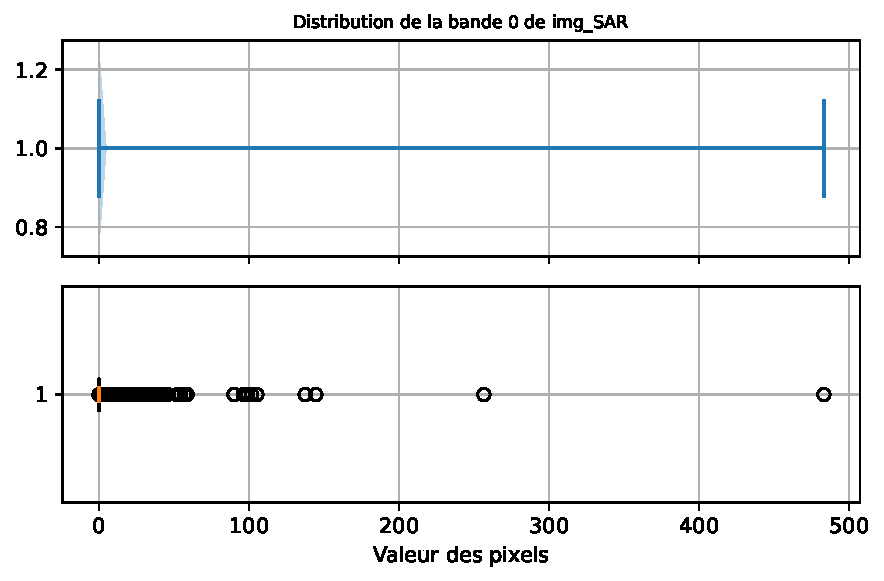
\includegraphics[keepaspectratio]{02-RehaussementVisualisationImages_files/figure-pdf/cell-19-output-1.pdf}}

Afin de visualiser correctement l'histogramme, il faut se limiter à un
intervalle de valeurs plus réduit. Dans le code ci-dessous, on impose à
la fonction \texttt{np.histogramme} de compter les valeurs de pixels
dans des intervalles de valeurs fixés par la fonction
\texttt{np.linspace(percentiles{[}0.1{]},percentiles{[}99.9{]},\ 50)} où
\texttt{percentiles{[}0.1{]}} et \texttt{percentiles{[}99.9{]}} sont les
\(0.1\%\) et \(99.9\%\) percentiles respectivement:

\begin{Shaded}
\begin{Highlighting}[]
\NormalTok{hist, bin\_edges }\OperatorTok{=}\NormalTok{ np.histogram(values, }
\NormalTok{                                bins}\OperatorTok{=}\NormalTok{np.linspace(percentiles[}\FloatTok{0.1}\NormalTok{], }
\NormalTok{                                percentiles[}\FloatTok{99.9}\NormalTok{], }\DecValTok{50}\NormalTok{), }
\NormalTok{                                density}\OperatorTok{=}\VariableTok{True}\NormalTok{)}

\NormalTok{fig, ax }\OperatorTok{=}\NormalTok{ plt.subplots(nrows}\OperatorTok{=}\DecValTok{2}\NormalTok{,ncols}\OperatorTok{=}\DecValTok{1}\NormalTok{,figsize}\OperatorTok{=}\NormalTok{(}\DecValTok{6}\NormalTok{, }\DecValTok{5}\NormalTok{), sharex}\OperatorTok{=}\VariableTok{True}\NormalTok{)}
\NormalTok{ax[}\DecValTok{0}\NormalTok{].bar(bin\_edges[:}\OperatorTok{{-}}\DecValTok{1}\NormalTok{], }
\NormalTok{                hist}\OperatorTok{*}\NormalTok{(bin\_edges[}\DecValTok{1}\NormalTok{]}\OperatorTok{{-}}\NormalTok{bin\_edges[}\DecValTok{0}\NormalTok{]), }
\NormalTok{                width}\OperatorTok{=}\NormalTok{ (bin\_edges[}\DecValTok{1}\NormalTok{]}\OperatorTok{{-}}\NormalTok{bin\_edges[}\DecValTok{0}\NormalTok{]), }
\NormalTok{                edgecolor}\OperatorTok{=} \StringTok{\textquotesingle{}w\textquotesingle{}}\NormalTok{)}
\NormalTok{ax[}\DecValTok{0}\NormalTok{].set\_title(}\StringTok{"Distribution de probabilité (PDF)"}\NormalTok{)}
\NormalTok{ax[}\DecValTok{0}\NormalTok{].set\_ylabel(}\StringTok{"Densité de probabilité"}\NormalTok{)}
\NormalTok{ax[}\DecValTok{0}\NormalTok{].grid(}\VariableTok{True}\NormalTok{)}

\NormalTok{ax[}\DecValTok{1}\NormalTok{].plot(bin\_edges[:}\OperatorTok{{-}}\DecValTok{1}\NormalTok{], }
\NormalTok{            hist.cumsum()}\OperatorTok{*}\NormalTok{(bin\_edges[}\DecValTok{1}\NormalTok{]}\OperatorTok{{-}}\NormalTok{bin\_edges[}\DecValTok{0}\NormalTok{]))}
\NormalTok{ax[}\DecValTok{1}\NormalTok{].set\_title(}\StringTok{"Distribution de probabilité cumulée (CDF)"}\NormalTok{)}
\NormalTok{ax[}\DecValTok{1}\NormalTok{].set\_xlabel(}\StringTok{"Valeur du pixel"}\NormalTok{)}
\NormalTok{ax[}\DecValTok{1}\NormalTok{].set\_ylabel(}\StringTok{"Probabilité cumulée"}\NormalTok{)}
\NormalTok{ax[}\DecValTok{1}\NormalTok{].grid(}\VariableTok{True}\NormalTok{)}
\NormalTok{plt.tight\_layout()}
\NormalTok{plt.show()                              }
\end{Highlighting}
\end{Shaded}

\pandocbounded{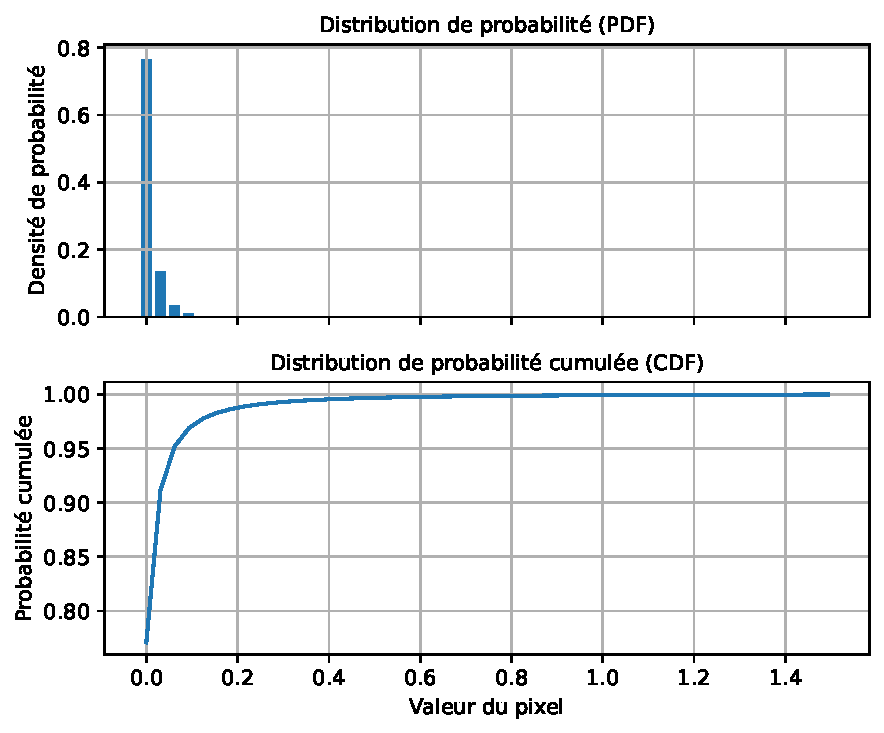
\includegraphics[keepaspectratio]{02-RehaussementVisualisationImages_files/figure-pdf/cell-20-output-1.pdf}}

Au niveau de l'affichage avec \texttt{matplotlib}, la dynamique peut
être contrôlée directement avec les paramètres \texttt{vmin} et
\texttt{vmax} comme ceci:

\begin{Shaded}
\begin{Highlighting}[]
\NormalTok{fig, ax }\OperatorTok{=}\NormalTok{ plt.subplots(nrows}\OperatorTok{=}\DecValTok{2}\NormalTok{, ncols}\OperatorTok{=}\DecValTok{2}\NormalTok{, figsize}\OperatorTok{=}\NormalTok{(}\DecValTok{6}\NormalTok{, }\DecValTok{5}\NormalTok{), sharex}\OperatorTok{=}\VariableTok{True}\NormalTok{, sharey}\OperatorTok{=}\VariableTok{True}\NormalTok{)}
\NormalTok{[a.axis(}\StringTok{\textquotesingle{}off\textquotesingle{}}\NormalTok{) }\ControlFlowTok{for}\NormalTok{ a }\KeywordTok{in}\NormalTok{ ax.flatten()]}
\NormalTok{ax[}\DecValTok{0}\NormalTok{,}\DecValTok{0}\NormalTok{].imshow(img\_SAR[}\DecValTok{0}\NormalTok{].values, vmin}\OperatorTok{=}\NormalTok{percentiles[}\DecValTok{0}\NormalTok{], vmax}\OperatorTok{=}\NormalTok{percentiles[}\DecValTok{100}\NormalTok{])}
\NormalTok{ax[}\DecValTok{0}\NormalTok{,}\DecValTok{0}\NormalTok{].set\_title(}\SpecialStringTok{f"0\% {-} 100\%=}\SpecialCharTok{\{}\NormalTok{percentiles[}\DecValTok{0}\NormalTok{]}\SpecialCharTok{:2.1f\}}\SpecialStringTok{ {-} }\SpecialCharTok{\{}\NormalTok{percentiles[}\DecValTok{100}\NormalTok{]}\SpecialCharTok{:2.1f\}}\SpecialStringTok{"}\NormalTok{)}
\NormalTok{ax[}\DecValTok{0}\NormalTok{,}\DecValTok{1}\NormalTok{].imshow(img\_SAR[}\DecValTok{0}\NormalTok{].values, vmin}\OperatorTok{=}\NormalTok{percentiles[}\FloatTok{0.1}\NormalTok{], vmax}\OperatorTok{=}\NormalTok{percentiles[}\FloatTok{99.9}\NormalTok{]) }
\NormalTok{ax[}\DecValTok{0}\NormalTok{,}\DecValTok{1}\NormalTok{].set\_title(}\SpecialStringTok{f"0.1\% {-} 99.9\%=}\SpecialCharTok{\{}\NormalTok{percentiles[}\FloatTok{0.1}\NormalTok{]}\SpecialCharTok{:2.1f\}}\SpecialStringTok{ {-} }\SpecialCharTok{\{}\NormalTok{percentiles[}\FloatTok{99.9}\NormalTok{]}\SpecialCharTok{:2.1f\}}\SpecialStringTok{"}\NormalTok{)}
\NormalTok{ax[}\DecValTok{1}\NormalTok{,}\DecValTok{0}\NormalTok{].imshow(img\_SAR[}\DecValTok{0}\NormalTok{].values, vmin}\OperatorTok{=}\NormalTok{percentiles[}\DecValTok{1}\NormalTok{], vmax}\OperatorTok{=}\NormalTok{percentiles[}\DecValTok{99}\NormalTok{]) }
\NormalTok{ax[}\DecValTok{1}\NormalTok{,}\DecValTok{0}\NormalTok{].set\_title(}\SpecialStringTok{f"1\% {-} 99\%=}\SpecialCharTok{\{}\NormalTok{percentiles[}\DecValTok{1}\NormalTok{]}\SpecialCharTok{:2.1f\}}\SpecialStringTok{ {-} }\SpecialCharTok{\{}\NormalTok{percentiles[}\DecValTok{99}\NormalTok{]}\SpecialCharTok{:2.1f\}}\SpecialStringTok{"}\NormalTok{)}
\NormalTok{ax[}\DecValTok{1}\NormalTok{,}\DecValTok{1}\NormalTok{].imshow(img\_SAR[}\DecValTok{0}\NormalTok{].values, vmin}\OperatorTok{=}\NormalTok{percentiles[}\DecValTok{2}\NormalTok{], vmax}\OperatorTok{=}\NormalTok{percentiles[}\DecValTok{98}\NormalTok{]) }
\NormalTok{ax[}\DecValTok{1}\NormalTok{,}\DecValTok{1}\NormalTok{].set\_title(}\SpecialStringTok{f"2\% {-} 98\%=}\SpecialCharTok{\{}\NormalTok{percentiles[}\DecValTok{2}\NormalTok{]}\SpecialCharTok{:2.1f\}}\SpecialStringTok{ {-} }\SpecialCharTok{\{}\NormalTok{percentiles[}\DecValTok{98}\NormalTok{]}\SpecialCharTok{:2.1f\}}\SpecialStringTok{"}\NormalTok{)}
\NormalTok{plt.tight\_layout()}
\end{Highlighting}
\end{Shaded}

\pandocbounded{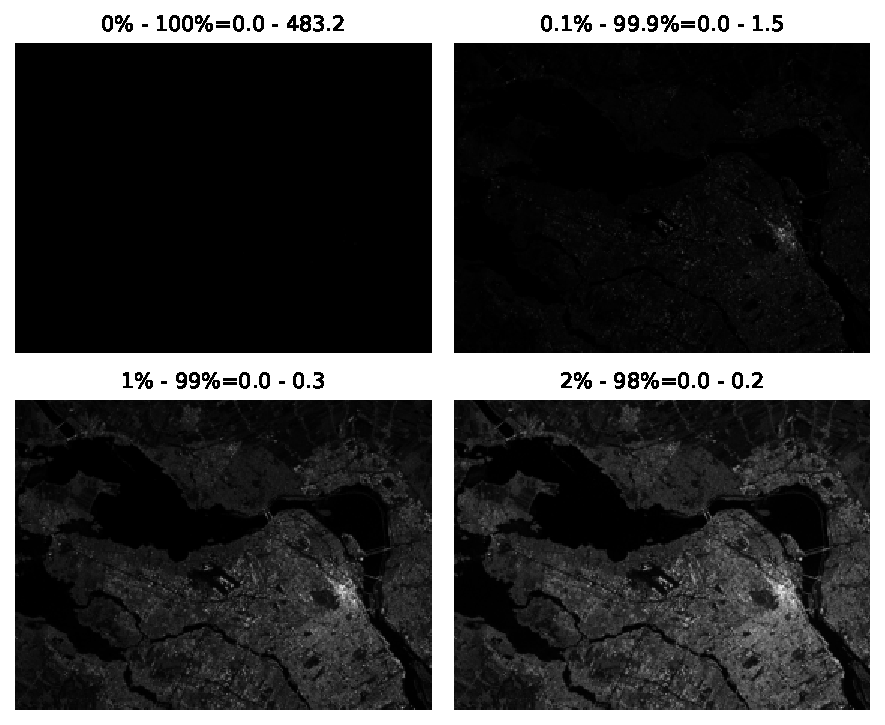
\includegraphics[keepaspectratio]{02-RehaussementVisualisationImages_files/figure-pdf/cell-21-output-1.pdf}}

\subsection{Réhaussements non
linéaires}\label{ruxe9haussements-non-linuxe9aires}

\subsubsection{Réhaussement par
fonctions}\label{ruxe9haussement-par-fonctions}

Le réhaussenent par fonction consiste à appliquer une fonction non
linéaire afin de modifier la dynamique de l'image. Par exemple, pour une
image radar, une transformation populaire est d'afficher les valeurs de
rétrodiffusion en décibel (\texttt{dB}) avec la fonction
\texttt{log10()}.

\begin{Shaded}
\begin{Highlighting}[]
\NormalTok{percentiles\_position}\OperatorTok{=}\NormalTok{ (}\DecValTok{0}\NormalTok{,}\FloatTok{0.1}\NormalTok{,}\DecValTok{1}\NormalTok{,}\DecValTok{2}\NormalTok{,}\DecValTok{50}\NormalTok{,}\DecValTok{98}\NormalTok{,}\DecValTok{99}\NormalTok{,}\FloatTok{99.9}\NormalTok{,}\DecValTok{100}\NormalTok{)}
\NormalTok{values}\OperatorTok{=} \DecValTok{10}\OperatorTok{*}\NormalTok{np.log10(img\_SAR[}\DecValTok{0}\NormalTok{]).data}
\NormalTok{percentiles\_db}\OperatorTok{=} \BuiltInTok{dict}\NormalTok{(}\BuiltInTok{zip}\NormalTok{(percentiles\_position, np.percentile(values, percentiles\_position)))}
\BuiltInTok{print}\NormalTok{(percentiles\_db)}
\end{Highlighting}
\end{Shaded}

\begin{verbatim}
{0: np.float64(-50.87641143798828), 0.1: np.float64(-47.98947440338135), 1: np.float64(-40.625951309204105), 2: np.float64(-37.24779266357422), 50: np.float64(-19.075313568115234), 98: np.float64(-7.6460519409179675), 99: np.float64(-5.534139237403945), 99.9: np.float64(1.8286541925668764), 100: np.float64(26.84148406982422)}
\end{verbatim}

Les boites à moustache (\emph{boxplots}) ont une bien meilleure
distribution qui est en effet très proche d'une distribution normale
gaussienne:

\pandocbounded{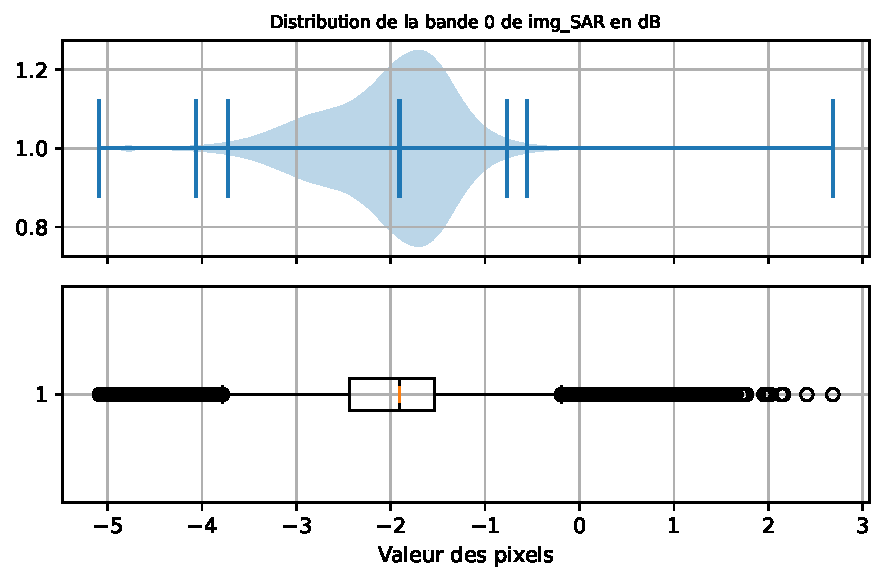
\includegraphics[keepaspectratio]{02-RehaussementVisualisationImages_files/figure-pdf/cell-23-output-1.pdf}}

On obtient ainsi les images suivantes:

\pandocbounded{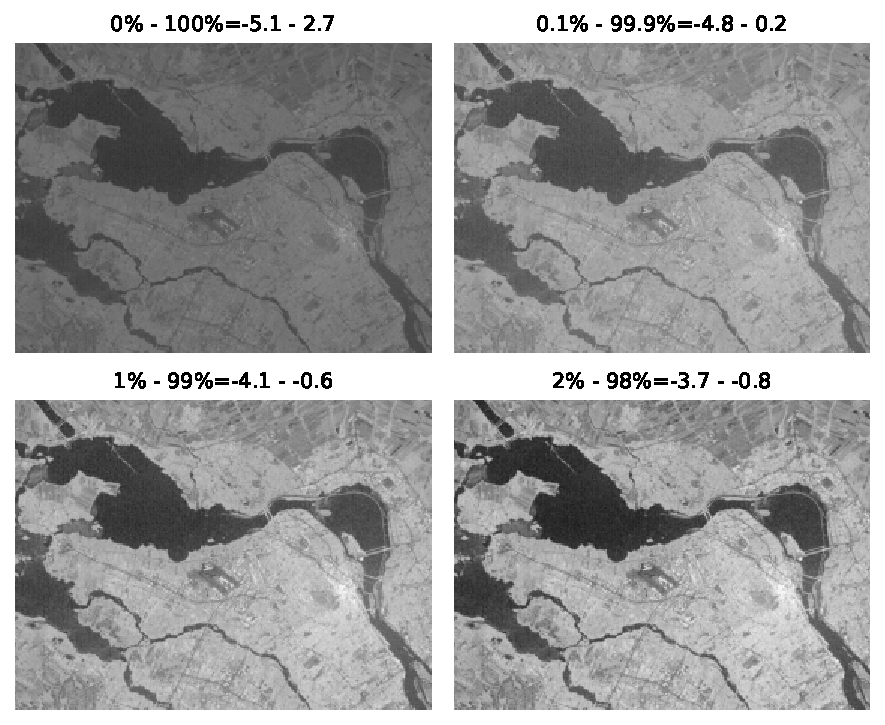
\includegraphics[keepaspectratio]{02-RehaussementVisualisationImages_files/figure-pdf/cell-24-output-1.pdf}}

\subsubsection{Égalisation
d'histogramme}\label{uxe9galisation-dhistogramme}

L'égalisation d'histogramme consiste à modifier les valeurs des pixels
d'une image source afin que la distribution cumulée des valeurs (CDF)
devienne similaire à celle d'une image cible. La CDF (\emph{Cumulative
Distribution Function}) est simplement la somme cumulée des valeurs de
l'histogramme:

\[
CDF_{source}(i)= \frac{1}{K}\sum_{j=0}^{j \leq i} hist_{source}(j)
\] avec \(K\) choisit de façon à ce que la dernière valeur soit égale à
1 (\(CDF_{source}(i_{max})=1\)). De la même manière, \(CDF_{cible}\) est
la CDF d'une image cible. La formule générale pour l'égalisation
d'histogramme est la suivante: \[
j = CDF_{cible}^{-1}(CDF_{source}(i))
\]

On peut choisir \(CDF_{cible}\) comme correspondant à une image où
chaque valeur de pixel est équiprobable (d'où le terme
\emph{égalisation}), ce qui veut dire \(hist_{cible}(j)=1/L\) avec \(L\)
égale au nombre de valeurs possibles dans l'image (par exemple
\(L=256\)). \[
j = L \times CDF_{source}(i)
\] On peut appliquer cette procédure sur l'image SAR en dB de la façon
suivante:

\begin{Shaded}
\begin{Highlighting}[]
\NormalTok{values}\OperatorTok{=}\NormalTok{ np.sort(np.log10(img\_SAR[}\DecValTok{0}\NormalTok{].data.flatten()))}
\NormalTok{cdf\_x}\OperatorTok{=}\NormalTok{ np.linspace(values[}\DecValTok{0}\NormalTok{], values[}\OperatorTok{{-}}\DecValTok{1}\NormalTok{], }\DecValTok{1000}\NormalTok{)}
\NormalTok{cdf\_source}\OperatorTok{=}\NormalTok{ np.interp(cdf\_x, values, np.arange(}\BuiltInTok{len}\NormalTok{(values))}\OperatorTok{/}\BuiltInTok{len}\NormalTok{(values)}\OperatorTok{*}\DecValTok{255}\NormalTok{)}
\NormalTok{values\_eq}\OperatorTok{=}\NormalTok{np.interp(np.log10(img\_SAR[}\DecValTok{0}\NormalTok{].data), cdf\_x, cdf\_source).astype(}\StringTok{\textquotesingle{}uint8\textquotesingle{}}\NormalTok{)}
\NormalTok{plt.imshow(values\_eq)}
\NormalTok{plt.axis(}\StringTok{\textquotesingle{}off\textquotesingle{}}\NormalTok{)}
\end{Highlighting}
\end{Shaded}

\pandocbounded{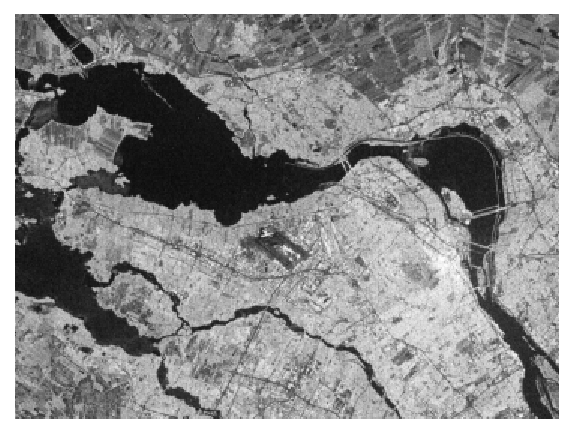
\includegraphics[keepaspectratio]{02-RehaussementVisualisationImages_files/figure-pdf/cell-25-output-1.pdf}}

\subsubsection{Palettes de couleur}\label{palettes-de-couleur}

Les palettes de couleurs sont appliquées dynamiquement à l'affichage sur
une image à une seule bande. La librairie \texttt{matplotlib} contient
un nombre considérable de
\href{https://matplotlib.org/stable/users/explain/colors/colormaps.html}{palettes}.

\begin{Shaded}
\begin{Highlighting}[]
\ImportTok{from}\NormalTok{ matplotlib }\ImportTok{import}\NormalTok{ colormaps}
\BuiltInTok{list}\NormalTok{(colormaps)}
\end{Highlighting}
\end{Shaded}

Voici quelques exemples ci-dessous, les valeurs de l'image doivent être
normalisées entre 0 et 1 ou entre 0 et 255 sinon les paramètres
\texttt{vmin} et \texttt{vmax} doivent être spécifiés. On peut observer
comment ces palettes révèlent les détails de l'image malgré une image
originalement très sombre.

\begin{Shaded}
\begin{Highlighting}[]
\NormalTok{fig, ax }\OperatorTok{=}\NormalTok{ plt.subplots(nrows}\OperatorTok{=}\DecValTok{2}\NormalTok{, ncols}\OperatorTok{=}\DecValTok{2}\NormalTok{, figsize}\OperatorTok{=}\NormalTok{(}\DecValTok{6}\NormalTok{, }\DecValTok{5}\NormalTok{), sharex}\OperatorTok{=}\VariableTok{True}\NormalTok{, sharey}\OperatorTok{=}\VariableTok{True}\NormalTok{)}
\NormalTok{[a.axis(}\StringTok{\textquotesingle{}off\textquotesingle{}}\NormalTok{) }\ControlFlowTok{for}\NormalTok{ a }\KeywordTok{in}\NormalTok{ ax.flatten()]}
\NormalTok{ax[}\DecValTok{0}\NormalTok{,}\DecValTok{0}\NormalTok{].imshow(img\_SAR[}\DecValTok{0}\NormalTok{].data, vmin}\OperatorTok{=}\NormalTok{percentiles[}\DecValTok{2}\NormalTok{], vmax}\OperatorTok{=}\NormalTok{percentiles[}\DecValTok{98}\NormalTok{], cmap}\OperatorTok{=}\StringTok{\textquotesingle{}jet\textquotesingle{}}\NormalTok{)}
\NormalTok{ax[}\DecValTok{0}\NormalTok{,}\DecValTok{0}\NormalTok{].set\_title(}\SpecialStringTok{f"jet"}\NormalTok{)}
\NormalTok{ax[}\DecValTok{0}\NormalTok{,}\DecValTok{1}\NormalTok{].imshow(img\_SAR[}\DecValTok{0}\NormalTok{].data, vmin}\OperatorTok{=}\NormalTok{percentiles[}\DecValTok{2}\NormalTok{], vmax}\OperatorTok{=}\NormalTok{percentiles[}\DecValTok{98}\NormalTok{], cmap}\OperatorTok{=}\StringTok{\textquotesingle{}hot\textquotesingle{}}\NormalTok{)}
\NormalTok{ax[}\DecValTok{0}\NormalTok{,}\DecValTok{1}\NormalTok{].set\_title(}\SpecialStringTok{f"hot"}\NormalTok{)}
\NormalTok{ax[}\DecValTok{1}\NormalTok{,}\DecValTok{0}\NormalTok{].imshow(img\_SAR[}\DecValTok{0}\NormalTok{].data, vmin}\OperatorTok{=}\NormalTok{percentiles[}\DecValTok{2}\NormalTok{], vmax}\OperatorTok{=}\NormalTok{percentiles[}\DecValTok{98}\NormalTok{], cmap}\OperatorTok{=}\StringTok{\textquotesingle{}hsv\textquotesingle{}}\NormalTok{)}
\NormalTok{ax[}\DecValTok{1}\NormalTok{,}\DecValTok{0}\NormalTok{].set\_title(}\SpecialStringTok{f"hsv"}\NormalTok{)}
\NormalTok{ax[}\DecValTok{1}\NormalTok{,}\DecValTok{1}\NormalTok{].imshow(img\_SAR[}\DecValTok{0}\NormalTok{].data, vmin}\OperatorTok{=}\NormalTok{percentiles[}\DecValTok{2}\NormalTok{], vmax}\OperatorTok{=}\NormalTok{percentiles[}\DecValTok{98}\NormalTok{], cmap}\OperatorTok{=}\StringTok{\textquotesingle{}terrain\textquotesingle{}}\NormalTok{)}
\NormalTok{ax[}\DecValTok{1}\NormalTok{,}\DecValTok{1}\NormalTok{].set\_title(}\SpecialStringTok{f"terrain"}\NormalTok{)}
\NormalTok{plt.tight\_layout()}
\end{Highlighting}
\end{Shaded}

\pandocbounded{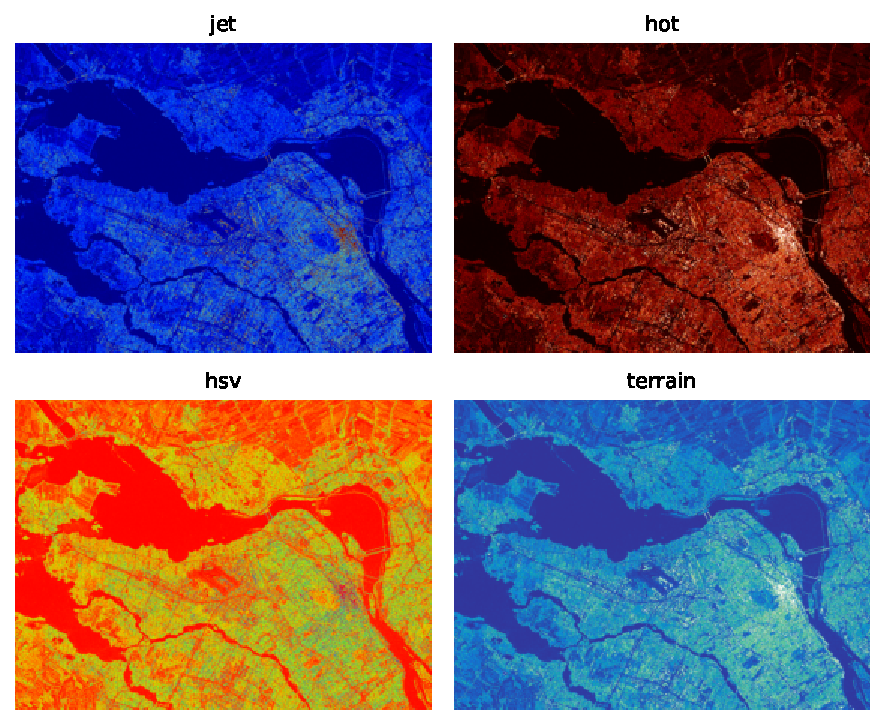
\includegraphics[keepaspectratio]{02-RehaussementVisualisationImages_files/figure-pdf/cell-27-output-1.pdf}}

Il peut être utile d'ajouter une barre de couleurs afin d'indiquer la
correspondance entre les couleurs et les valeurs numériques:

\begin{Shaded}
\begin{Highlighting}[]
\ImportTok{import}\NormalTok{ matplotlib }\ImportTok{as}\NormalTok{ mpl}
\NormalTok{fig, ax }\OperatorTok{=}\NormalTok{ plt.subplots(figsize}\OperatorTok{=}\NormalTok{(}\DecValTok{6}\NormalTok{, }\DecValTok{6}\NormalTok{))}
\NormalTok{cmap}\OperatorTok{=}\NormalTok{ mpl.colormaps.get\_cmap(}\StringTok{\textquotesingle{}jet\textquotesingle{}}\NormalTok{).with\_extremes(under}\OperatorTok{=}\StringTok{\textquotesingle{}white\textquotesingle{}}\NormalTok{, over}\OperatorTok{=}\StringTok{\textquotesingle{}magenta\textquotesingle{}}\NormalTok{)}
\NormalTok{h}\OperatorTok{=}\NormalTok{plt.imshow(img\_SAR[}\DecValTok{0}\NormalTok{].data, norm}\OperatorTok{=}\NormalTok{mpl.colors.LogNorm(vmin}\OperatorTok{=}\NormalTok{percentiles[}\DecValTok{2}\NormalTok{], vmax}\OperatorTok{=}\NormalTok{percentiles[}\DecValTok{98}\NormalTok{]),}
\NormalTok{                   cmap}\OperatorTok{=}\NormalTok{cmap)}
\NormalTok{fig.colorbar(h, ax}\OperatorTok{=}\NormalTok{ax,  orientation}\OperatorTok{=}\StringTok{\textquotesingle{}horizontal\textquotesingle{}}\NormalTok{, label}\OperatorTok{=}\StringTok{"Intensité"}\NormalTok{, extend}\OperatorTok{=}\StringTok{\textquotesingle{}both\textquotesingle{}}\NormalTok{)}
\NormalTok{ax.axis(}\StringTok{\textquotesingle{}off\textquotesingle{}}\NormalTok{) }
\end{Highlighting}
\end{Shaded}

\pandocbounded{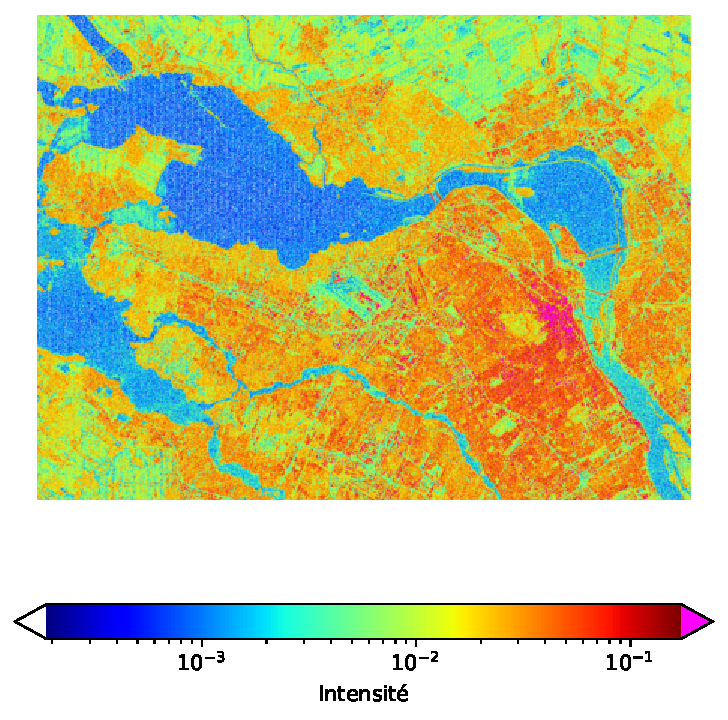
\includegraphics[keepaspectratio]{02-RehaussementVisualisationImages_files/figure-pdf/cell-28-output-1.pdf}}

\subsection{Composés colorés}\label{composuxe9s-coloruxe9s}

Le système visuel humain est sensible seulement à la partie visible du
spectre électromagnétique qui compose les couleurs de l'arc-en-ciel du
bleu au rouge. L'ensemble des couleurs du spectre visible peut être
obtenu à partir du mélange de trois couleurs primaires (rouge, vert et
bleu). Ce système de décomposition à trois couleurs est à la base de la
plupart des systèmes de visualisation ou de représentation de
l'information de couleur. Si on prend le cas des images Sentinel-2, 12
bandes sont disponibles, plusieurs composés couleurs sont donc possibles
(voir le site de
\href{https://custom-scripts.sentinel-hub.com/custom-scripts/sentinel-2/composites/}{Copernicus}).
Voici quelques exemples possibles, chaque composé mettant en valeur des
propriétés différentes de la surface.

\begin{Shaded}
\begin{Highlighting}[]
\ImportTok{import}\NormalTok{ rioxarray }\ImportTok{as}\NormalTok{ rxr}
\NormalTok{fig, ax}\OperatorTok{=}\NormalTok{ plt.subplots(nrows}\OperatorTok{=}\DecValTok{2}\NormalTok{, ncols}\OperatorTok{=} \DecValTok{2}\NormalTok{, figsize}\OperatorTok{=}\NormalTok{(}\DecValTok{8}\NormalTok{, }\DecValTok{6}\NormalTok{), sharex}\OperatorTok{=}\VariableTok{True}\NormalTok{, sharey}\OperatorTok{=}\VariableTok{True}\NormalTok{)}
\NormalTok{img\_s2.sel(band}\OperatorTok{=}\NormalTok{[}\DecValTok{4}\NormalTok{,}\DecValTok{3}\NormalTok{,}\DecValTok{2}\NormalTok{]).plot.imshow(vmin}\OperatorTok{=}\DecValTok{86}\NormalTok{, vmax}\OperatorTok{=}\DecValTok{4000}\NormalTok{, ax}\OperatorTok{=}\NormalTok{ax[}\DecValTok{0}\NormalTok{,}\DecValTok{0}\NormalTok{])}
\NormalTok{ax[}\DecValTok{0}\NormalTok{,}\DecValTok{0}\NormalTok{].set\_title(}\StringTok{\textquotesingle{}RVB\textquotesingle{}}\NormalTok{)}
\NormalTok{img\_s2.sel(band}\OperatorTok{=}\NormalTok{[}\DecValTok{8}\NormalTok{,}\DecValTok{3}\NormalTok{,}\DecValTok{2}\NormalTok{]).plot.imshow(vmin}\OperatorTok{=}\DecValTok{86}\NormalTok{, vmax}\OperatorTok{=}\DecValTok{4000}\NormalTok{, ax}\OperatorTok{=}\NormalTok{ax[}\DecValTok{0}\NormalTok{,}\DecValTok{1}\NormalTok{])}
\NormalTok{ax[}\DecValTok{0}\NormalTok{,}\DecValTok{1}\NormalTok{].set\_title(}\StringTok{\textquotesingle{}NIR,V,B\textquotesingle{}}\NormalTok{)}
\NormalTok{img\_s2.sel(band}\OperatorTok{=}\NormalTok{[}\DecValTok{12}\NormalTok{,}\DecValTok{8}\NormalTok{,}\DecValTok{4}\NormalTok{]).plot.imshow(vmin}\OperatorTok{=}\DecValTok{86}\NormalTok{, vmax}\OperatorTok{=}\DecValTok{4000}\NormalTok{, ax}\OperatorTok{=}\NormalTok{ax[}\DecValTok{1}\NormalTok{,}\DecValTok{0}\NormalTok{])}
\NormalTok{ax[}\DecValTok{1}\NormalTok{,}\DecValTok{0}\NormalTok{].set\_title(}\StringTok{\textquotesingle{}SWIR2,NIR,R\textquotesingle{}}\NormalTok{)}
\NormalTok{img\_s2.sel(band}\OperatorTok{=}\NormalTok{[}\DecValTok{12}\NormalTok{,}\DecValTok{11}\NormalTok{,}\DecValTok{4}\NormalTok{]).plot.imshow(vmin}\OperatorTok{=}\DecValTok{86}\NormalTok{, vmax}\OperatorTok{=}\DecValTok{4000}\NormalTok{, ax}\OperatorTok{=}\NormalTok{ax[}\DecValTok{1}\NormalTok{,}\DecValTok{1}\NormalTok{])}
\NormalTok{ax[}\DecValTok{1}\NormalTok{,}\DecValTok{1}\NormalTok{].set\_title(}\StringTok{\textquotesingle{}SWIR2,SWIR1,NIR\textquotesingle{}}\NormalTok{)}
\NormalTok{plt.tight\_layout()}
\NormalTok{plt.show()}
\end{Highlighting}
\end{Shaded}

\pandocbounded{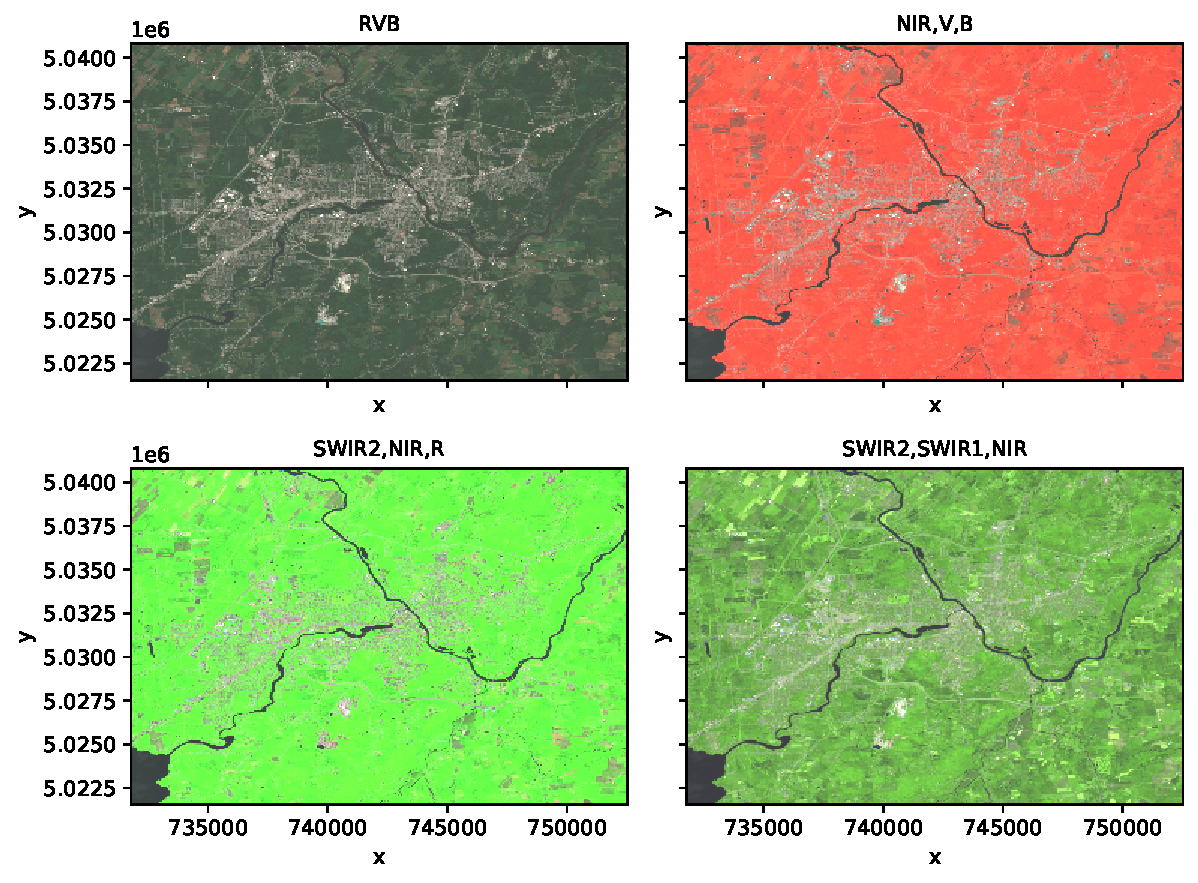
\includegraphics[keepaspectratio]{02-RehaussementVisualisationImages_files/figure-pdf/cell-29-output-1.pdf}}

\part{Partie 2. Transformations des données satellitaires}

\bookmarksetup{startatroot}

\chapter{Transformations spectrales}\label{sec-chap03}

\section{Préambule}\label{pruxe9ambule-2}

Assurez-vous de lire ce préambule avant d'exécuter le reste du notebook.

\subsection{Objectifs}\label{objectifs-2}

Dans ce chapitre, nous abordons l'exploitation de la dimension spectrale
des images satellites. Ce chapitre est aussi disponible sous la forme
d'un notebook Python:

\href{https://colab.research.google.com/github/sfoucher/TraitementImagesPythonVol1/blob/main/notebooks/03-TransformationSpectrales.ipynb}{\pandocbounded{
\includegraphics[keepaspectratio]{images/colab.png}}}

\begin{tcolorbox}[colback=background_color, colframe=objectif_color, boxrule=0.2mm, leftrule=1mm, coltitle=black, fonttitle=\bfseries, title={
\includegraphics[width=0.3cm]{images/BlocObjectif.png} \textbf{Objectif}}]

\textbf{Objectifs d'apprentissage visés dans ce chapitre}

À la fin de ce chapitre, vous devriez être en mesure de~:

\begin{itemize}
\tightlist
\item
  comprendre le principe des indices spectraux;
\item
  calculer différents indices avec spyndex;
\item
  analyser le gain en information des indices;
\end{itemize}

\end{tcolorbox}

\subsection{Librairies}\label{librairies}

Les librairies qui vont être explorées dans ce chapitre sont les
suivantes:

\begin{itemize}
\item
  \href{https://scipy.org/}{SciPy}
\item
  \href{https://numpy.org/}{NumPy}
\item
  \href{https://github.com/awesome-spectral-indices/spyndex}{spyindex}
\item
  \href{https://rasterio.readthedocs.io/en/stable/}{Rasterio}
\item
  \href{https://docs.xarray.dev/en/stable/}{Xarray}
\item
  \href{https://corteva.github.io/rioxarray/stable/index.html}{rioxarray}
\end{itemize}

Dans l'environnement Google Colab, seul \texttt{rioxarray} doit être
installés

\begin{Shaded}
\begin{Highlighting}[]
\OperatorTok{\%\%}\NormalTok{capture}
\OperatorTok{!}\NormalTok{pip install }\OperatorTok{{-}}\NormalTok{qU matplotlib rioxarray xrscipy scikit}\OperatorTok{{-}}\NormalTok{image pyarrow spyndex}
\end{Highlighting}
\end{Shaded}

Vérifiez les importations:

\begin{Shaded}
\begin{Highlighting}[]
\ImportTok{import}\NormalTok{ numpy }\ImportTok{as}\NormalTok{ np}
\ImportTok{import}\NormalTok{ rioxarray }\ImportTok{as}\NormalTok{ rxr}
\ImportTok{from}\NormalTok{ scipy }\ImportTok{import}\NormalTok{ signal}
\ImportTok{import}\NormalTok{ xarray }\ImportTok{as}\NormalTok{ xr}
\ImportTok{import}\NormalTok{ xrscipy}
\ImportTok{import}\NormalTok{ matplotlib.pyplot }\ImportTok{as}\NormalTok{ plt}
\ImportTok{import}\NormalTok{ spyndex}
\ImportTok{import}\NormalTok{ rasterio }\ImportTok{as}\NormalTok{ rio}
\end{Highlighting}
\end{Shaded}

\subsection{Images utilisées}\label{images-utilisuxe9es}

Nous utilisons les images suivantes dans ce chapitre:

\begin{Shaded}
\begin{Highlighting}[]
\OperatorTok{\%\%}\NormalTok{capture}
\ImportTok{import}\NormalTok{ gdown}

\NormalTok{gdown.download(}\StringTok{\textquotesingle{}https://drive.google.com/uc?export=download\&confirm=pbef\&id=1a6Ypg0g1Oy4AJt9XWKWfnR12NW1XhNg\_\textquotesingle{}}\NormalTok{, output}\OperatorTok{=} \StringTok{\textquotesingle{}RGBNIR\_of\_S2A.tif\textquotesingle{}}\NormalTok{)}
\NormalTok{gdown.download(}\StringTok{\textquotesingle{}https://drive.google.com/uc?export=download\&confirm=pbef\&id=1a6O3L\_abOfU7h94K22At8qtBuLMGErwo\textquotesingle{}}\NormalTok{, output}\OperatorTok{=} \StringTok{\textquotesingle{}sentinel2.tif\textquotesingle{}}\NormalTok{)}
\NormalTok{gdown.download(}\StringTok{\textquotesingle{}https://drive.google.com/uc?export=download\&confirm=pbef\&id=1\_zwCLN{-}x7XJcNHJCH6Z8upEdUXtVtvs1\textquotesingle{}}\NormalTok{, output}\OperatorTok{=} \StringTok{\textquotesingle{}berkeley.jpg\textquotesingle{}}\NormalTok{)}
\NormalTok{gdown.download(}\StringTok{\textquotesingle{}https://drive.google.com/uc?export=download\&confirm=pbef\&id=1dM6IVqjba6GHwTLmI7CpX8GP2z5txUq6\textquotesingle{}}\NormalTok{, output}\OperatorTok{=} \StringTok{\textquotesingle{}SAR.tif\textquotesingle{}}\NormalTok{)}
\NormalTok{gdown.download(}\StringTok{\textquotesingle{}https://drive.google.com/uc?export=download\&confirm=pbef\&id=1aAq7crc\_LoaLC3kG3HkQ6Fv5JfG0mswg\textquotesingle{}}\NormalTok{, output}\OperatorTok{=} \StringTok{\textquotesingle{}carte.tif\textquotesingle{}}\NormalTok{)}
\NormalTok{gdown.download(}\StringTok{\textquotesingle{}https://drive.google.com/uc?export=download\&confirm=pbef\&id=1iCZNYTv0qEZRzPhe22nPdpV4Ks7NsY3b\textquotesingle{}}\NormalTok{, output}\OperatorTok{=} \StringTok{\textquotesingle{}ASCIIdata\_splib07b\_rsSentinel2.zip\textquotesingle{}}\NormalTok{)}
\OperatorTok{!}\NormalTok{unzip }\OperatorTok{{-}}\NormalTok{q ASCIIdata\_splib07b\_rsSentinel2.}\BuiltInTok{zip}
\end{Highlighting}
\end{Shaded}

Vérifiez que vous êtes capable de les lire :

\begin{Shaded}
\begin{Highlighting}[]
\ControlFlowTok{with}\NormalTok{ rxr.open\_rasterio(}\StringTok{\textquotesingle{}berkeley.jpg\textquotesingle{}}\NormalTok{, mask\_and\_scale}\OperatorTok{=} \VariableTok{True}\NormalTok{) }\ImportTok{as}\NormalTok{ img\_rgb:}
    \BuiltInTok{print}\NormalTok{(img\_rgb)}
\ControlFlowTok{with}\NormalTok{ rxr.open\_rasterio(}\StringTok{\textquotesingle{}RGBNIR\_of\_S2A.tif\textquotesingle{}}\NormalTok{, mask\_and\_scale}\OperatorTok{=} \VariableTok{True}\NormalTok{) }\ImportTok{as}\NormalTok{ img\_rgbnir:}
    \BuiltInTok{print}\NormalTok{(img\_rgbnir)}
\ControlFlowTok{with}\NormalTok{ rxr.open\_rasterio(}\StringTok{\textquotesingle{}sentinel2.tif\textquotesingle{}}\NormalTok{, mask\_and\_scale}\OperatorTok{=} \VariableTok{True}\NormalTok{) }\ImportTok{as}\NormalTok{ img\_s2:}
    \BuiltInTok{print}\NormalTok{(img\_s2)}
\ControlFlowTok{with}\NormalTok{ rxr.open\_rasterio(}\StringTok{\textquotesingle{}carte.tif\textquotesingle{}}\NormalTok{, mask\_and\_scale}\OperatorTok{=} \VariableTok{True}\NormalTok{) }\ImportTok{as}\NormalTok{ img\_carte:}
    \BuiltInTok{print}\NormalTok{(img\_carte)}
\end{Highlighting}
\end{Shaded}

\section{Qu'est ce que l'information
spectrale?}\label{quest-ce-que-linformation-spectrale}

L'information spectrale touche à l'exploitation de la dimension
spectrale des images (c.à.d le long des bandes spectrales de l'image).
La taille de cette dimension spectrale dépend du type de capteurs
considéré. Un capteur à très haute résolution spectrale par exemple aura
très peu de bandes (4 ou 5). Un capteur multispectral pourra contenir
une quinzaine de bande. À l'autre extrême, on trouvera les capteurs
hyperspectraux qui peuvent contenir des centaines de bandes spectrales.

\begin{figure}[H]

{\centering 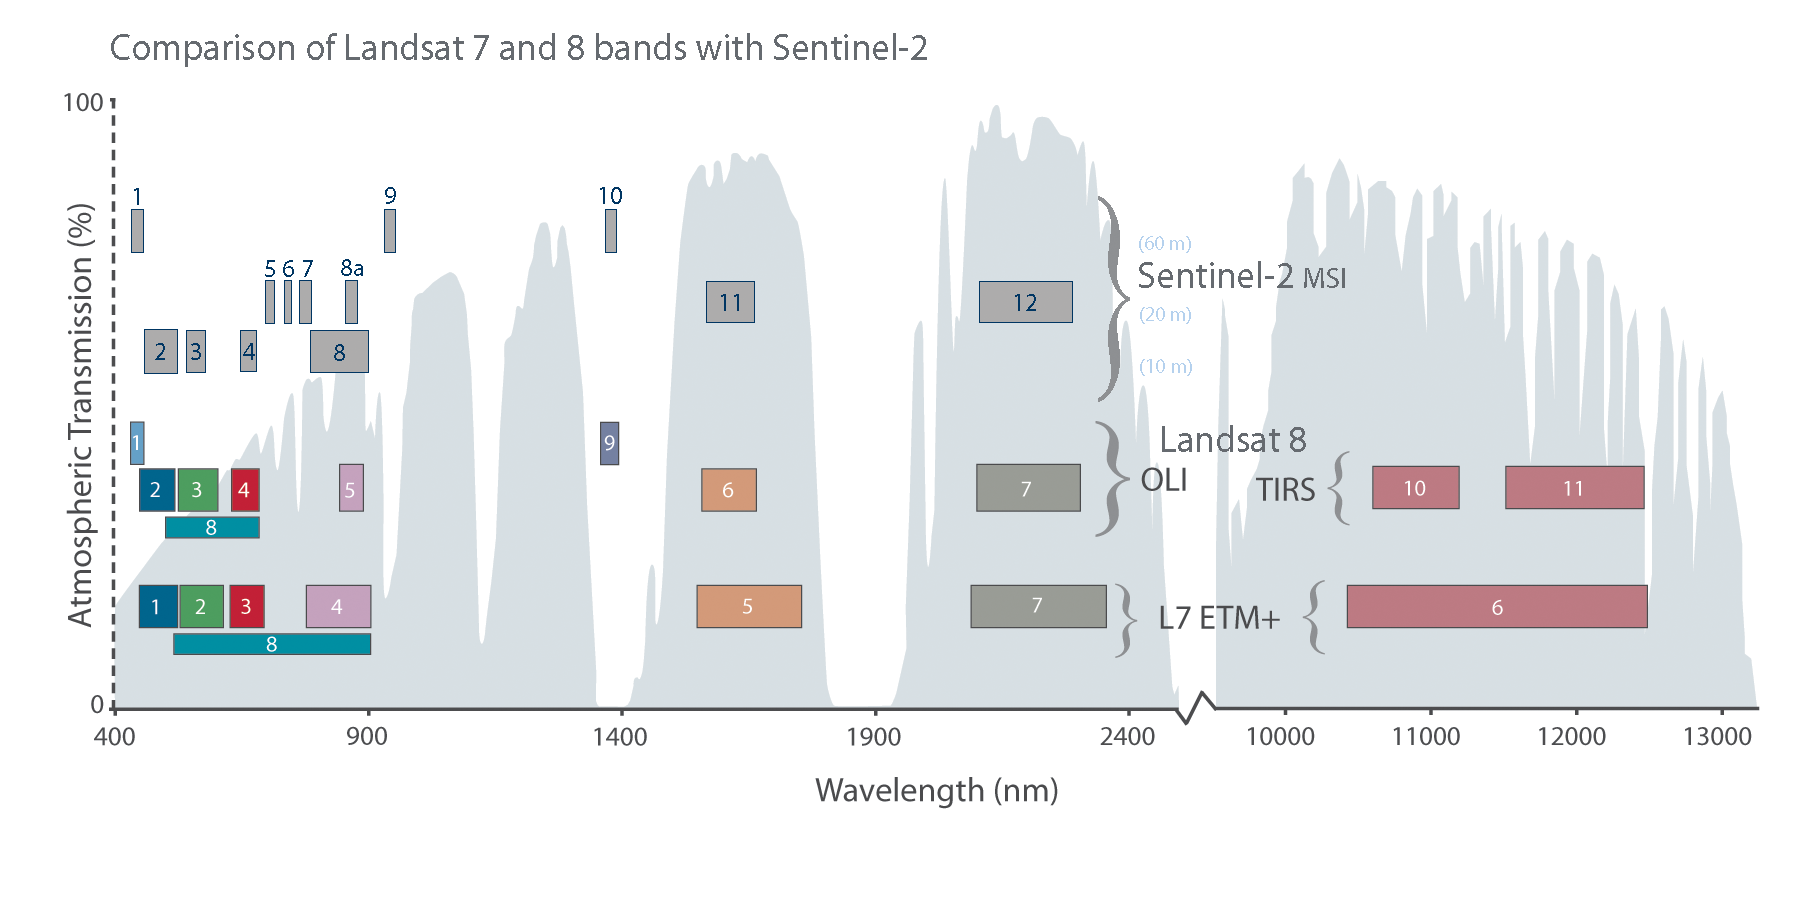
\includegraphics[width=6in,height=\textheight,keepaspectratio]{images/Landsat.v.Sentinel-2-1.png}

}

\caption{Positions des bandes spectrales pour quelques capteurs
(\href{https://landsat.gsfc.nasa.gov/article/sentinel-2a-launches-our-compliments-our-complements/}{source})}

\end{figure}%

Pour une surface donnée, la forme des valeurs le long de l'axe spectrale
caractérise le type de matériau observé ainsi que son état. On parle
souvent alors de signature spectrale. On peut voir celle-ci comme une
généralisation de la couleur d'un matériau au delà des bandes visibles
du spectre. L'exploitation de ces signatures spectrales est probablement
un des principes les plus importants en télédétection qui le distingue
de la vison par ordinateur.
L'\href{https://www.sciencebase.gov/catalog/item/586e8c88e4b0f5ce109fccae}{USGS}
maintient une base de données spectrales acquises en laboratoire (Kokaly
et Klein 2017). On peut observer sur la figure ci-dessous comment la
forme et l'amplitude de trois signatures différentes peut changer en
fonction du type de surface.

\begin{verbatim}
Text(0, 0.5, 'Réflectance')
\end{verbatim}

Exemples de signatures spectrales pour trois surfaces différentes pour
les bandes spectrales de Sentinel-2

\pandocbounded{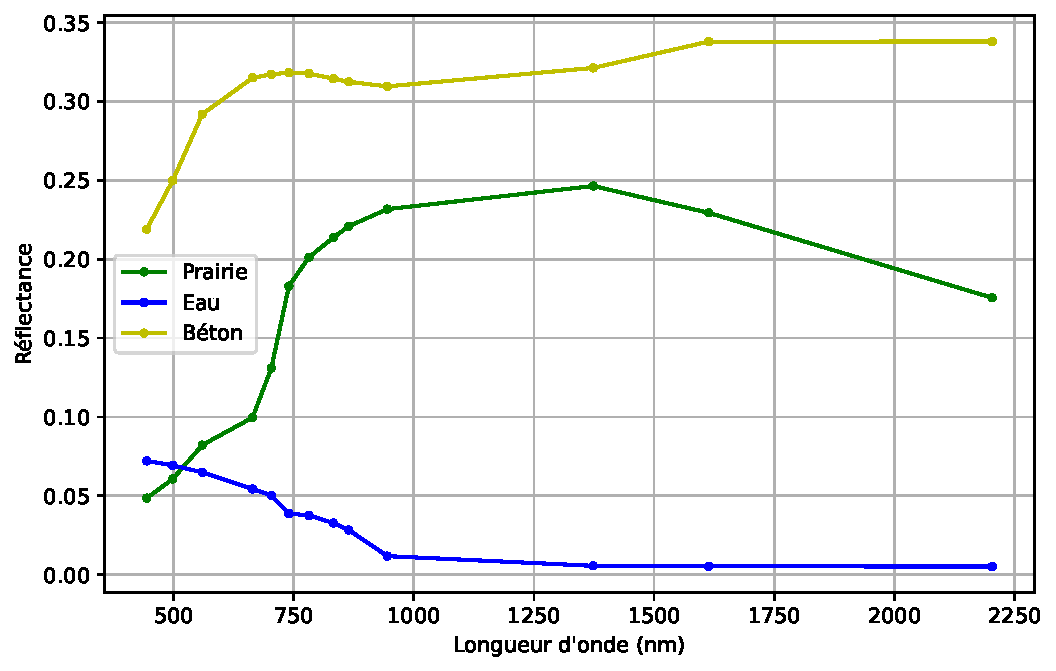
\includegraphics[keepaspectratio]{03-TransformationSpectrales_files/figure-pdf/cell-7-output-2.pdf}}

\section{Indices spectraux}\label{indices-spectraux}

Il existe une vaste littérature sur les indices spectraux, le choix d'un
indice plutôt qu'un autre dépend fortement de l'application visée, nous
allons simplement couvrir les principes de base ici. Le principe d'un
indice spectral consiste à mettre en valeur certaines caractéristiques
saillantes du spectre comme des pentes, des gradients, etc.

La librairie Python
\href{https://awesome-ee-spectral-indices.readthedocs.io/en/latest/}{Awesome
Spectral Indices} maintient une liste de plus de 200 indices spectraux
(radar et optiques). La liste complète est affichable avec la commande
suivante:

\begin{Shaded}
\begin{Highlighting}[]
\NormalTok{spyndex.indices}
\end{Highlighting}
\end{Shaded}

\begin{verbatim}
SpectralIndices(['AFRI1600', 'AFRI2100', 'ANDWI', 'ARI', 'ARI2', 'ARVI', 'ATSAVI', 'AVI', 'AWEInsh', 'AWEIsh', 'BAI', 'BAIM', 'BAIS2', 'BCC', 'BI', 'BITM', 'BIXS', 'BLFEI', 'BNDVI', 'BRBA', 'BWDRVI', 'BaI', 'CCI', 'CIG', 'CIRE', 'CRI550', 'CRI700', 'CSI', 'CSIT', 'CVI', 'DBI', 'DBSI', 'DPDD', 'DSI', 'DSWI1', 'DSWI2', 'DSWI3', 'DSWI4', 'DSWI5', 'DVI', 'DVIplus', 'DpRVIHH', 'DpRVIVV', 'EBBI', 'EBI', 'EMBI', 'ENDVI', 'EVI', 'EVI2', 'EVIv', 'ExG', 'ExGR', 'ExR', 'FAI', 'FCVI', 'GARI', 'GBNDVI', 'GCC', 'GDVI', 'GEMI', 'GLI', 'GM1', 'GM2', 'GNDVI', 'GOSAVI', 'GRNDVI', 'GRVI', 'GSAVI', 'GVMI', 'IAVI', 'IBI', 'IKAW', 'IPVI', 'IRECI', 'LSWI', 'MBI', 'MBWI', 'MCARI', 'MCARI1', 'MCARI2', 'MCARI705', 'MCARIOSAVI', 'MCARIOSAVI705', 'MGRVI', 'MIRBI', 'MLSWI26', 'MLSWI27', 'MNDVI', 'MNDWI', 'MNLI', 'MRBVI', 'MSAVI', 'MSI', 'MSR', 'MSR705', 'MTCI', 'MTVI1', 'MTVI2', 'MuWIR', 'NBAI', 'NBLI', 'NBLIOLI', 'NBR', 'NBR2', 'NBRSWIR', 'NBRT1', 'NBRT2', 'NBRT3', 'NBRplus', 'NBSIMS', 'NBUI', 'ND705', 'NDBI', 'NDBaI', 'NDCI', 'NDDI', 'NDGI', 'NDGlaI', 'NDII', 'NDISIb', 'NDISIg', 'NDISImndwi', 'NDISIndwi', 'NDISIr', 'NDMI', 'NDPI', 'NDPolI', 'NDPonI', 'NDREI', 'NDSI', 'NDSII', 'NDSIWV', 'NDSInw', 'NDSWIR', 'NDSaII', 'NDSoI', 'NDTI', 'NDVI', 'NDVI705', 'NDVIMNDWI', 'NDVIT', 'NDWI', 'NDWIns', 'NDYI', 'NGRDI', 'NHFD', 'NIRv', 'NIRvH2', 'NIRvP', 'NLI', 'NMDI', 'NRFIg', 'NRFIr', 'NSDS', 'NSDSI1', 'NSDSI2', 'NSDSI3', 'NSTv1', 'NSTv2', 'NWI', 'NormG', 'NormNIR', 'NormR', 'OCVI', 'OSAVI', 'OSI', 'PI', 'PISI', 'PSRI', 'QpRVI', 'RCC', 'RDVI', 'REDSI', 'RENDVI', 'RFDI', 'RGBVI', 'RGRI', 'RI', 'RI4XS', 'RNDVI', 'RVI', 'S2REP', 'S2WI', 'S3', 'SARVI', 'SAVI', 'SAVI2', 'SAVIT', 'SEVI', 'SI', 'SIPI', 'SLAVI', 'SR', 'SR2', 'SR3', 'SR555', 'SR705', 'SWI', 'SWM', 'SeLI', 'TCARI', 'TCARIOSAVI', 'TCARIOSAVI705', 'TCI', 'TDVI', 'TGI', 'TRRVI', 'TSAVI', 'TTVI', 'TVI', 'TWI', 'TriVI', 'UI', 'VARI', 'VARI700', 'VDDPI', 'VHVVD', 'VHVVP', 'VHVVR', 'VI6T', 'VI700', 'VIBI', 'VIG', 'VVVHD', 'VVVHR', 'VVVHS', 'VgNIRBI', 'VrNIRBI', 'WDRVI', 'WDVI', 'WI1', 'WI2', 'WI2015', 'WRI', 'bNIRv', 'kEVI', 'kIPVI', 'kNDVI', 'kRVI', 'kVARI', 'mND705', 'mSR705', 'sNIRvLSWI', 'sNIRvNDPI', 'sNIRvNDVILSWIP', 'sNIRvNDVILSWIS', 'sNIRvSWIR'])
\end{verbatim}

Le détail d'un indice particulier, par exemple le `NDVI`, est aussi
affichable:

\begin{Shaded}
\begin{Highlighting}[]
\NormalTok{spyndex.indices[}\StringTok{"NDVI"}\NormalTok{]}
\end{Highlighting}
\end{Shaded}

\begin{verbatim}
SpectralIndex(NDVI: Normalized Difference Vegetation Index)
        * Application Domain: vegetation
        * Bands/Parameters: ['N', 'R']
        * Formula: (N-R)/(N+R)
        * Reference: https://ntrs.nasa.gov/citations/19740022614
        
\end{verbatim}

\texttt{spyndex} pré-suppose une nomenclature prédéfinie des
\href{https://awesome-ee-spectral-indices.readthedocs.io/en/latest/\#expressions}{bandes},
on peut voir la correspondance sur le tableau ci-dessous:

\begin{Shaded}
\begin{Highlighting}[]
\NormalTok{spyndex.bands}
\end{Highlighting}
\end{Shaded}

\begin{verbatim}
Bands(['A', 'B', 'G', 'G1', 'N', 'N2', 'R', 'RE1', 'RE2', 'RE3', 'S1', 'S2', 'T', 'T1', 'T2', 'WV', 'Y'])
\end{verbatim}

\begin{longtable}[]{@{}llll@{}}
\caption{Noms des bandes Sentinel-2}\tabularnewline
\toprule\noalign{}
Index & Noms & Spyndex & Noms \\
\midrule\noalign{}
\endfirsthead
\toprule\noalign{}
Index & Noms & Spyndex & Noms \\
\midrule\noalign{}
\endhead
\bottomrule\noalign{}
\endlastfoot
1 & B01 & A & Aérosol \\
2 & B02 & B & Bleu \\
3 & B03 & G & Vert \\
4 & B04 & R & Rouge \\
5 & B05 & RE1 & Red edge 1 \\
6 & B06 & RE1 & Red edge 2 \\
7 & B07 & RE2 & Red edge 3 \\
8 & B08 & N & Proche-infrarouge 1 \\
9 & B08A & N2 & Proche-infrarouge 2 \\
10 & B09 & - & Vapeur d'eau \\
11 & B11 & S1 & Infra-rouge onde courte 1 \\
12 & B12 & S2 & Infra-rouge onde courte 1 \\
\end{longtable}

Deux options sont possibles, on peut soit renommer les noms des bandes
avec \texttt{xarray} ou ``mapper'' les noms vers les noms appropriés.
Regardons les dimensions de notre jeux de données:

\begin{Shaded}
\begin{Highlighting}[]
\NormalTok{img\_s2.dims}
\end{Highlighting}
\end{Shaded}

\begin{verbatim}
('band', 'y', 'x')
\end{verbatim}

On peut simplement changer les index (\texttt{coords}) de la dimension
\texttt{band}:

\begin{Shaded}
\begin{Highlighting}[]
\NormalTok{img\_s2 }\OperatorTok{=}\NormalTok{ img\_s2.sel(band }\OperatorTok{=} \BuiltInTok{list}\NormalTok{(}\BuiltInTok{range}\NormalTok{(}\DecValTok{1}\NormalTok{,}\DecValTok{13}\NormalTok{))).assign\_coords(\{}\StringTok{\textquotesingle{}band\textquotesingle{}}\NormalTok{:[}\StringTok{"A"}\NormalTok{, }\StringTok{"B"}\NormalTok{, }\StringTok{"G"}\NormalTok{, }\StringTok{"R"}\NormalTok{, }\StringTok{"RE1"}\NormalTok{, }\StringTok{"RE2"}\NormalTok{, }\StringTok{"RE3"}\NormalTok{, }\StringTok{"N"}\NormalTok{, }\StringTok{"N2"}\NormalTok{, }\StringTok{"WV"}\NormalTok{, }\StringTok{"S1"}\NormalTok{, }\StringTok{"S2"}\NormalTok{]\})}
\NormalTok{img\_s2}\OperatorTok{=}\NormalTok{img\_s2}\OperatorTok{/}\DecValTok{10000} \CommentTok{\# normalisation en réflectance}
\end{Highlighting}
\end{Shaded}

\begin{Shaded}
\begin{Highlighting}[]
\ImportTok{from}\NormalTok{ rasterio }\ImportTok{import}\NormalTok{ plot}
\NormalTok{idx }\OperatorTok{=}\NormalTok{ spyndex.computeIndex(}
\NormalTok{    index }\OperatorTok{=}\NormalTok{ [}\StringTok{"NDVI"}\NormalTok{,}\StringTok{"GNDVI"}\NormalTok{,}\StringTok{"SAVI"}\NormalTok{],}
\NormalTok{    params }\OperatorTok{=}\NormalTok{ \{}
        \StringTok{"N"}\NormalTok{: img\_s2.sel(band }\OperatorTok{=} \StringTok{"N"}\NormalTok{),}
        \StringTok{"R"}\NormalTok{: img\_s2.sel(band }\OperatorTok{=} \StringTok{"R"}\NormalTok{),}
        \StringTok{"G"}\NormalTok{: img\_s2.sel(band }\OperatorTok{=} \StringTok{"G"}\NormalTok{),}
        \StringTok{"L"}\NormalTok{: }\FloatTok{0.5}
\NormalTok{    \}}
\NormalTok{)}

\CommentTok{\# Plot the indices (and the RGB image for comparison)}
\NormalTok{fig, ax }\OperatorTok{=}\NormalTok{ plt.subplots(}\DecValTok{2}\NormalTok{,}\DecValTok{2}\NormalTok{,figsize }\OperatorTok{=}\NormalTok{ (}\DecValTok{9}\NormalTok{,}\DecValTok{9}\NormalTok{))}
\NormalTok{[a.axis(}\StringTok{\textquotesingle{}off\textquotesingle{}}\NormalTok{) }\ControlFlowTok{for}\NormalTok{ a }\KeywordTok{in}\NormalTok{ ax.flatten()]}
\NormalTok{plot.show(img\_s2.sel(band }\OperatorTok{=}\NormalTok{ [}\StringTok{"R"}\NormalTok{,}\StringTok{"G"}\NormalTok{,}\StringTok{"B"}\NormalTok{]).data }\OperatorTok{/} \FloatTok{0.3}\NormalTok{,ax }\OperatorTok{=}\NormalTok{ ax[}\DecValTok{0}\NormalTok{,}\DecValTok{0}\NormalTok{],title }\OperatorTok{=} \StringTok{"RGB"}\NormalTok{)}
\NormalTok{plot.show(idx.sel(index }\OperatorTok{=} \StringTok{"NDVI"}\NormalTok{),ax }\OperatorTok{=}\NormalTok{ ax[}\DecValTok{0}\NormalTok{,}\DecValTok{1}\NormalTok{],title }\OperatorTok{=} \StringTok{"NDVI"}\NormalTok{)}
\NormalTok{plot.show(idx.sel(index }\OperatorTok{=} \StringTok{"GNDVI"}\NormalTok{),ax }\OperatorTok{=}\NormalTok{ ax[}\DecValTok{1}\NormalTok{,}\DecValTok{0}\NormalTok{],title }\OperatorTok{=} \StringTok{"GNDVI"}\NormalTok{)}
\NormalTok{plot.show(idx.sel(index }\OperatorTok{=} \StringTok{"SAVI"}\NormalTok{),ax }\OperatorTok{=}\NormalTok{ ax[}\DecValTok{1}\NormalTok{,}\DecValTok{1}\NormalTok{],title }\OperatorTok{=} \StringTok{"SAVI"}\NormalTok{)}
\end{Highlighting}
\end{Shaded}

\pandocbounded{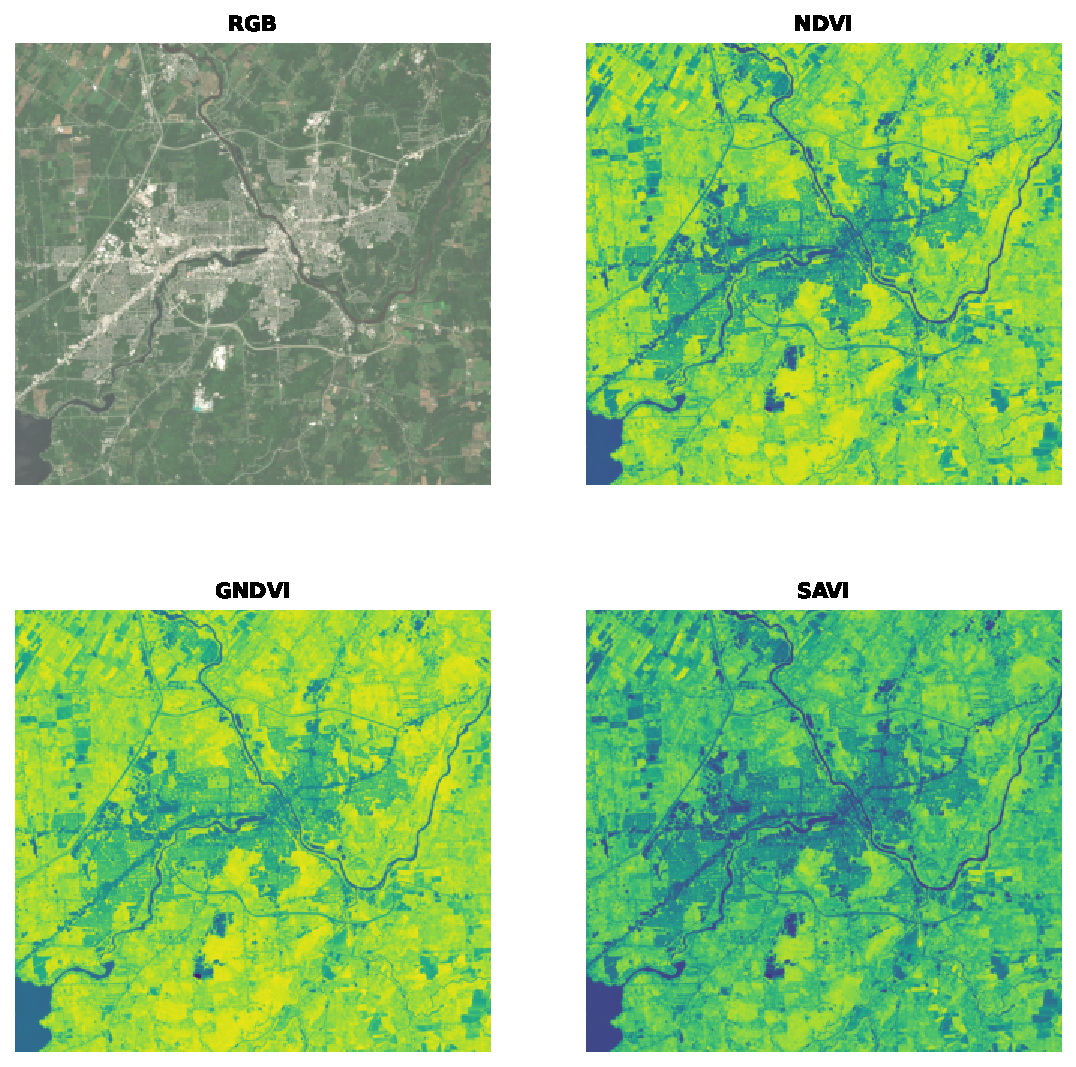
\includegraphics[keepaspectratio]{03-TransformationSpectrales_files/figure-pdf/cell-13-output-1.pdf}}

On peut vérifier l'utilité des indices en vérifiant leur séparabilité
pour certaines classes d'intérêts. Nous reprenons ici l'exemple de la
section section~\ref{sec-05.02.02} pour vérifier l'utilité des indices
\texttt{NDVI}, \texttt{NDWI} et \texttt{NDBI}:

\begin{Shaded}
\begin{Highlighting}[]
\ImportTok{import}\NormalTok{ pandas }\ImportTok{as}\NormalTok{ pd}
\ImportTok{import}\NormalTok{ seaborn }\ImportTok{as}\NormalTok{ sns}

\CommentTok{\# On sélectionne trois classes}
\NormalTok{class\_selected}\OperatorTok{=}\NormalTok{ [}\DecValTok{1}\NormalTok{,}\DecValTok{3}\NormalTok{,}\DecValTok{9}\NormalTok{]}
\NormalTok{df}\OperatorTok{=}\NormalTok{ pd.concat([gdf[gdf[}\StringTok{\textquotesingle{}class\textquotesingle{}}\NormalTok{] }\OperatorTok{==}\NormalTok{c] }\ControlFlowTok{for}\NormalTok{ c }\KeywordTok{in}\NormalTok{ class\_selected], ignore\_index}\OperatorTok{=}\VariableTok{True}\NormalTok{)}
\NormalTok{idx[}\StringTok{"Land Cover"}\NormalTok{] }\OperatorTok{=}\NormalTok{ [nom\_classes[l] }\ControlFlowTok{for}\NormalTok{ l }\KeywordTok{in}\NormalTok{ df[}\StringTok{"class"}\NormalTok{].tolist()]}
\CommentTok{\# Compute the desired spectral indices}
\NormalTok{idx }\OperatorTok{=}\NormalTok{ spyndex.computeIndex(}
\NormalTok{    index }\OperatorTok{=}\NormalTok{ [}\StringTok{"NDVI"}\NormalTok{,}\StringTok{"NDWI"}\NormalTok{,}\StringTok{"NDBI"}\NormalTok{],}
\NormalTok{    params }\OperatorTok{=}\NormalTok{ \{}
        \StringTok{"N"}\NormalTok{: df[}\StringTok{"SR\_B8"}\NormalTok{],}
        \StringTok{"R"}\NormalTok{: df[}\StringTok{"SR\_B4"}\NormalTok{],}
        \StringTok{"G"}\NormalTok{: df[}\StringTok{"SR\_B3"}\NormalTok{],}
        \StringTok{"S1"}\NormalTok{: df[}\StringTok{"SR\_B11"}\NormalTok{]}
\NormalTok{    \}}
\NormalTok{)}

\NormalTok{colors}\OperatorTok{=}\NormalTok{ [couleurs\_classes[c] }\ControlFlowTok{for}\NormalTok{ c }\KeywordTok{in}\NormalTok{ class\_selected]}
\CommentTok{\# Plot a pairplot to check the indices behaviour}
\NormalTok{plt.figure(figsize }\OperatorTok{=}\NormalTok{ (}\DecValTok{15}\NormalTok{,}\DecValTok{15}\NormalTok{))}
\NormalTok{g }\OperatorTok{=}\NormalTok{ sns.PairGrid(idx,hue }\OperatorTok{=} \StringTok{"Land Cover"}\NormalTok{,palette }\OperatorTok{=}\NormalTok{ sns.color\_palette(colors))}
\NormalTok{g.map\_lower(sns.scatterplot)}
\NormalTok{g.map\_upper(sns.kdeplot,fill }\OperatorTok{=} \VariableTok{True}\NormalTok{,alpha }\OperatorTok{=} \FloatTok{.5}\NormalTok{)}
\NormalTok{g.map\_diag(sns.kdeplot,fill }\OperatorTok{=} \VariableTok{True}\NormalTok{)}
\NormalTok{g.add\_legend()}
\NormalTok{plt.show()}
\end{Highlighting}
\end{Shaded}

\begin{figure}[H]

{\centering \pandocbounded{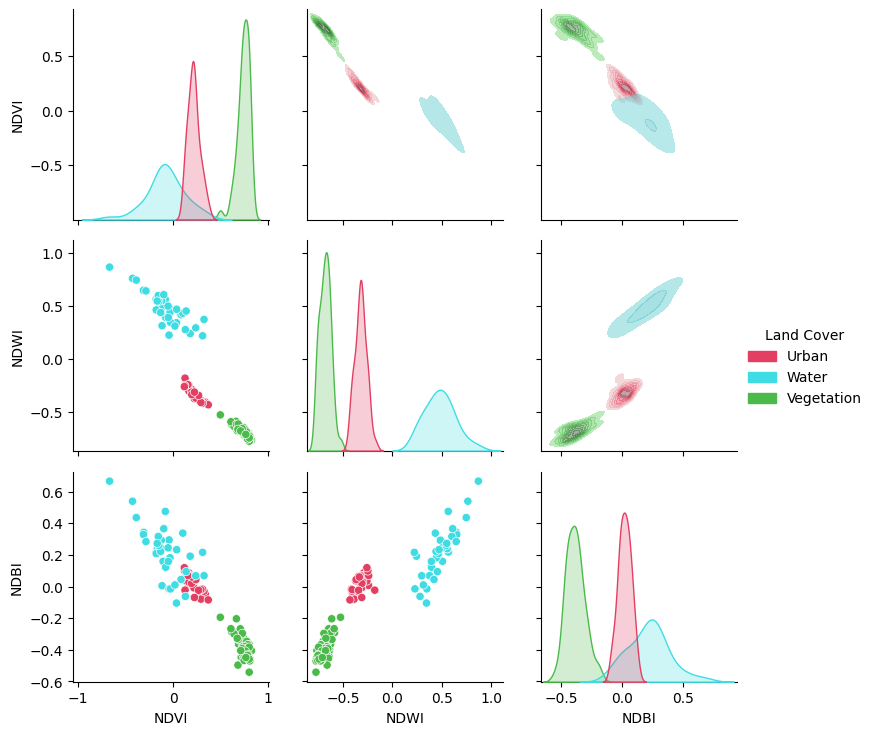
\includegraphics[keepaspectratio]{images/fig-classes-indices.png}}

}

\caption{Visualisation des points d'une image Sentinel-2 pour trois
classes}

\end{figure}%

\bookmarksetup{startatroot}

\chapter{Transformations spatiales}\label{sec-chap04}

\section{Préambule}\label{pruxe9ambule-3}

Assurez-vous de lire ce préambule avant d'exécuter le reste du notebook.

\subsection{Objectifs}\label{objectifs-3}

Dans ce chapitre, nous abordons quelques techniques de traitement
d'images dans le domaine spatial uniquement. Ce chapitre est aussi
disponible sous la forme d'un notebook Python sur Google Colab:

\href{https://colab.research.google.com/github/sfoucher/TraitementImagesPythonVol1/blob/main/notebooks/04-TransformationSpatiales.ipynb}{\pandocbounded{
\includegraphics[keepaspectratio]{images/colab.png}}}

\begin{tcolorbox}[colback=background_color, colframe=objectif_color, boxrule=0.2mm, leftrule=1mm, coltitle=black, fonttitle=\bfseries, title={
\includegraphics[width=0.3cm]{images/BlocObjectif.png} \textbf{Objectif}}]

\textbf{Objectifs d'apprentissage visés dans ce chapitre}

À la fin de ce chapitre, vous devriez être en mesure de~:

\begin{itemize}
\tightlist
\item
  comprendre le principe de la décomposition de Fourier;
\item
  comprendre le principe de la convolution;
\item
  appliquer un filtrage local à l'aide d'une fenêtre;
\item
  segmenter une image en super-pixels et calculer leurs propriétés
\end{itemize}

\end{tcolorbox}

\subsection{Librairies}\label{librairies-1}

Les librairies utilisées dans ce chapitre sont les suivantes:

\begin{itemize}
\item
  \href{https://scipy.org/}{SciPy}
\item
  \href{https://numpy.org/}{NumPy}
\item
  \href{https://pypi.org/project/opencv-python/}{opencv-python · PyPI}
\item
  \href{https://scikit-image.org/}{scikit-image}
\item
  \href{https://rasterio.readthedocs.io/en/stable/}{Rasterio}
\item
  \href{https://docs.xarray.dev/en/stable/}{Xarray}
\item
  \href{https://corteva.github.io/rioxarray/stable/index.html}{rioxarray}
\end{itemize}

Dans l'environnement Google Colab, seul \texttt{rioxarray} doit être
installé:

\begin{Shaded}
\begin{Highlighting}[]
\OperatorTok{\%\%}\NormalTok{capture}
\OperatorTok{!}\NormalTok{pip install }\OperatorTok{{-}}\NormalTok{qU matplotlib rioxarray xrscipy scikit}\OperatorTok{{-}}\NormalTok{image}
\end{Highlighting}
\end{Shaded}

Vérifiez les importations:

\begin{Shaded}
\begin{Highlighting}[]
\ImportTok{import}\NormalTok{ numpy }\ImportTok{as}\NormalTok{ np}
\ImportTok{import}\NormalTok{ numpy.fft}
\ImportTok{import}\NormalTok{ rioxarray }\ImportTok{as}\NormalTok{ rxr}
\ImportTok{from}\NormalTok{ scipy }\ImportTok{import}\NormalTok{ signal, ndimage}
\ImportTok{import}\NormalTok{ xarray }\ImportTok{as}\NormalTok{ xr}
\ImportTok{import}\NormalTok{ xrscipy}
\ImportTok{import}\NormalTok{ matplotlib.pyplot }\ImportTok{as}\NormalTok{ plt}
\ImportTok{from}\NormalTok{ skimage }\ImportTok{import}\NormalTok{ data, measure, graph, segmentation, color}
\ImportTok{from}\NormalTok{ skimage.color }\ImportTok{import}\NormalTok{ rgb2gray}
\ImportTok{from}\NormalTok{ skimage.segmentation }\ImportTok{import}\NormalTok{ slic, mark\_boundaries}
\ImportTok{import}\NormalTok{ pandas }\ImportTok{as}\NormalTok{ pd}
\end{Highlighting}
\end{Shaded}

\subsection{Images utilisées}\label{images-utilisuxe9es-1}

Nous utilisons les images suivantes dans ce chapitre:

\begin{Shaded}
\begin{Highlighting}[]
\OperatorTok{\%\%}\NormalTok{capture}
\ImportTok{import}\NormalTok{ gdown}

\NormalTok{gdown.download(}\StringTok{\textquotesingle{}https://drive.google.com/uc?export=download\&confirm=pbef\&id=1a6Ypg0g1Oy4AJt9XWKWfnR12NW1XhNg\_\textquotesingle{}}\NormalTok{, output}\OperatorTok{=} \StringTok{\textquotesingle{}RGBNIR\_of\_S2A.tif\textquotesingle{}}\NormalTok{)}
\NormalTok{gdown.download(}\StringTok{\textquotesingle{}https://drive.google.com/uc?export=download\&confirm=pbef\&id=1a4PQ68Ru8zBphbQ22j0sgJ4D2quw{-}Wo6\textquotesingle{}}\NormalTok{, output}\OperatorTok{=} \StringTok{\textquotesingle{}landsat7.tif\textquotesingle{}}\NormalTok{)}
\NormalTok{gdown.download(}\StringTok{\textquotesingle{}https://drive.google.com/uc?export=download\&confirm=pbef\&id=1\_zwCLN{-}x7XJcNHJCH6Z8upEdUXtVtvs1\textquotesingle{}}\NormalTok{, output}\OperatorTok{=} \StringTok{\textquotesingle{}berkeley.jpg\textquotesingle{}}\NormalTok{)}
\NormalTok{gdown.download(}\StringTok{\textquotesingle{}https://drive.google.com/uc?export=download\&confirm=pbef\&id=1dM6IVqjba6GHwTLmI7CpX8GP2z5txUq6\textquotesingle{}}\NormalTok{, output}\OperatorTok{=} \StringTok{\textquotesingle{}SAR.tif\textquotesingle{}}\NormalTok{)}
\end{Highlighting}
\end{Shaded}

Vérifiez que vous êtes capable de les lire :

\begin{Shaded}
\begin{Highlighting}[]
\ControlFlowTok{with}\NormalTok{ rxr.open\_rasterio(}\StringTok{\textquotesingle{}berkeley.jpg\textquotesingle{}}\NormalTok{, mask\_and\_scale}\OperatorTok{=} \VariableTok{True}\NormalTok{) }\ImportTok{as}\NormalTok{ img\_rgb:}
    \BuiltInTok{print}\NormalTok{(img\_rgb)}
\ControlFlowTok{with}\NormalTok{ rxr.open\_rasterio(}\StringTok{\textquotesingle{}RGBNIR\_of\_S2A.tif\textquotesingle{}}\NormalTok{, mask\_and\_scale}\OperatorTok{=} \VariableTok{True}\NormalTok{) }\ImportTok{as}\NormalTok{ img\_rgbnir:}
    \BuiltInTok{print}\NormalTok{(img\_rgbnir)}
\ControlFlowTok{with}\NormalTok{ rxr.open\_rasterio(}\StringTok{\textquotesingle{}SAR.tif\textquotesingle{}}\NormalTok{, mask\_and\_scale}\OperatorTok{=} \VariableTok{True}\NormalTok{) }\ImportTok{as}\NormalTok{ img\_SAR:}
    \BuiltInTok{print}\NormalTok{(img\_SAR)}
\end{Highlighting}
\end{Shaded}

\section{Analyse fréquentielle}\label{analyse-fruxe9quentielle}

L'analyse fréquentielle, issue du traitement du signal, permet d'avoir
un autre point de vue sur les données à partir de ses composantes
harmoniques. La modification de ces composantes de Fourier modifie
l'ensemble de l'image et permet de corriger des problèmes systématiques
comme des artefacts ou du bruit de capteur. Bien que ce domaine soit un
peu éloigné de la télédétection, les images issues des capteurs sont
toutes sujettes à des étapes de traitement du signal et il faut donc en
connaître les grands principes afin de pouvoir comprendre certains
enjeux lors des traitements.

\subsection{La transformée de
Fourier}\label{la-transformuxe9e-de-fourier}

La transformée de Fourier permet de transformer une image dans un espace
fréquentielle. Cette transformée est complètement réversible. Dans le
cas des images numériques, on parle de \texttt{2D-DFT}
(\emph{2D-Discrete Fourier Transform}) qui est un algorithme optimisé
pour le calcul fréquentiel (Cooley et Tukey 1965). La \emph{1D-DFT} peu
s'écrire simplement comme une projection sur une série d'exponentielles
complexes:

\begin{equation}\phantomsection\label{eq-dft}{X[k] = \sum_{n=0 \ldots N-1} x[n] \times \exp(-j \times 2\pi \times k \times n/N))}\end{equation}

La transformée inverse prend une forme similaire:

\begin{equation}\phantomsection\label{eq-idft}{x[k] = \frac{1}{N}\sum_{n=0 \ldots N-1} X[n] \times \exp(j \times 2\pi \times k \times n/N))}\end{equation}

Le signal d'origine est donc reconstruit à partir d'une somme de
sinusoïdes complexes \(\exp(j2\pi \frac{k}{N}n))\) de fréquence \(k/N\).
Noter qu'à partir de \(k=N/2\), les sinusoïdes se répètent à un signe
près et forme un miroir des composantes, la convention est alors de
mettre ces composantes dans une espace négatif \([-N/2,\ldots,-1]\).

Dans le cas d'un simple signal périodique à une dimension avec une
fréquence de 4/16 (donc 4 périodes sur 16) on obtient deux pics de
fréquence à la position de 4 cycles observés sur \(N=16\) observations.
Les puissances de Fourier sont affichées dans un espace fréquentiel en
cycles par unité d'espacement de l'échantillon (avec zéro au début)
variant entre -1 et +1. Par exemple, si l'espacement des échantillons
est en secondes, l'unité de fréquence est cycles/seconde (ou Hz). Dans
le cas de N échantillons, le pic sera observé à la fréquence
\(+/- 4/16=0.25\) cycles/secondes. La fréquence d'échantillonnage
\(F_s\) du signal a aussi beaucoup d'importance aussi et doit être au
moins a deux fois la plus haute fréquence observée (ici \(F_s > 0.5\))
sinon un phénomène de repliement appelé aliasing sera observé.

\begin{Shaded}
\begin{Highlighting}[]
\ImportTok{import}\NormalTok{ math}
\NormalTok{Fs}\OperatorTok{=} \FloatTok{2.0}
\NormalTok{Ts}\OperatorTok{=} \DecValTok{1}\OperatorTok{/}\NormalTok{Fs}
\NormalTok{N}\OperatorTok{=} \DecValTok{16}
\NormalTok{arr }\OperatorTok{=}\NormalTok{ xr.DataArray(np.sin(}\DecValTok{2}\OperatorTok{*}\NormalTok{math.pi}\OperatorTok{*}\NormalTok{np.arange(}\DecValTok{0}\NormalTok{,N,Ts)}\OperatorTok{*}\DecValTok{4}\OperatorTok{/}\DecValTok{16}\NormalTok{),}
\NormalTok{                   dims}\OperatorTok{=}\NormalTok{(}\StringTok{\textquotesingle{}x\textquotesingle{}}\NormalTok{), coords}\OperatorTok{=}\NormalTok{\{}\StringTok{\textquotesingle{}x\textquotesingle{}}\NormalTok{: np.arange(}\DecValTok{0}\NormalTok{,N,Ts)\})}
\NormalTok{fourier }\OperatorTok{=}\NormalTok{ np.fft.fft(arr)}
\NormalTok{freq }\OperatorTok{=}\NormalTok{ np.fft.fftfreq(fourier.size, d}\OperatorTok{=}\NormalTok{Ts)}
\NormalTok{fourier }\OperatorTok{=}\NormalTok{ xr.DataArray(fourier,}
\NormalTok{                   dims}\OperatorTok{=}\NormalTok{(}\StringTok{\textquotesingle{}f\textquotesingle{}}\NormalTok{), coords}\OperatorTok{=}\NormalTok{\{}\StringTok{\textquotesingle{}f\textquotesingle{}}\NormalTok{: freq\})}

\NormalTok{fig, axes }\OperatorTok{=}\NormalTok{ plt.subplots(nrows}\OperatorTok{=}\DecValTok{1}\NormalTok{, ncols}\OperatorTok{=}\DecValTok{2}\NormalTok{, figsize}\OperatorTok{=}\NormalTok{(}\DecValTok{10}\NormalTok{, }\DecValTok{4}\NormalTok{))}
\NormalTok{plt.subplot(}\DecValTok{1}\NormalTok{, }\DecValTok{2}\NormalTok{, }\DecValTok{1}\NormalTok{)}
\NormalTok{arr.plot.line(color}\OperatorTok{=}\StringTok{\textquotesingle{}red\textquotesingle{}}\NormalTok{, linestyle}\OperatorTok{=}\StringTok{\textquotesingle{}dashed\textquotesingle{}}\NormalTok{, marker}\OperatorTok{=}\StringTok{\textquotesingle{}o\textquotesingle{}}\NormalTok{, markerfacecolor}\OperatorTok{=}\StringTok{\textquotesingle{}blue\textquotesingle{}}\NormalTok{)}
\NormalTok{axes[}\DecValTok{0}\NormalTok{].set\_title(}\StringTok{"Signal périodique"}\NormalTok{)}
\NormalTok{plt.subplot(}\DecValTok{1}\NormalTok{, }\DecValTok{2}\NormalTok{, }\DecValTok{2}\NormalTok{)}
\NormalTok{np.}\BuiltInTok{abs}\NormalTok{(fourier).plot.line(color}\OperatorTok{=}\StringTok{\textquotesingle{}red\textquotesingle{}}\NormalTok{, linestyle}\OperatorTok{=}\StringTok{\textquotesingle{}dashed\textquotesingle{}}\NormalTok{, marker}\OperatorTok{=}\StringTok{\textquotesingle{}o\textquotesingle{}}\NormalTok{, markerfacecolor}\OperatorTok{=}\StringTok{\textquotesingle{}blue\textquotesingle{}}\NormalTok{)}
\NormalTok{axes[}\DecValTok{1}\NormalTok{].set\_title(}\StringTok{"Composantes de Fourier (amplitude)"}\NormalTok{)}
\NormalTok{plt.show()}
\end{Highlighting}
\end{Shaded}

\pandocbounded{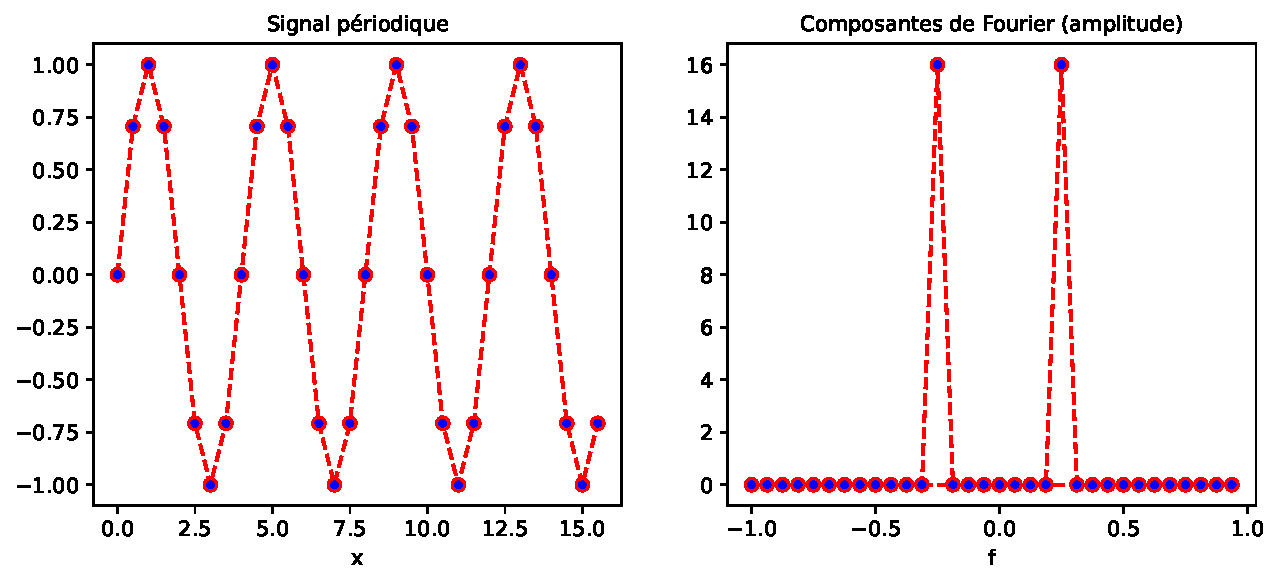
\includegraphics[keepaspectratio]{04-TransformationSpatiales_files/figure-pdf/cell-7-output-1.pdf}}

\subsection{Filtrage fréquentiel}\label{filtrage-fruxe9quentiel}

Un filtrage fréquentiel consiste à modifier le spectre de Fourier afin
d'éliminer ou de réduire certaines composantes fréquentielles. On
distingue habituellement trois catégories de filtres fréquentiels:

\begin{enumerate}
\def\labelenumi{\arabic{enumi}.}
\item
  Les filtres passe-bas qui ne préservent que les basses fréquences
  pour, par exemple, lisser une image.
\item
  Les filtres passe-hauts qui ne préservent que les hautes fréquences
  pour ne préserver que les détails.
\item
  Les filtres passe-bandes qui vont préserver les fréquences dans une
  bande de fréquence particulière.
\end{enumerate}

La librairie \texttt{Scipy} contient différents filtres fréquentiels.
Notez, qu'un filtrage fréquentielle est une simple multiplication de la
réponse du filtre \(F[k]\) par les composantes fréquentielles du signal
à filtrer \(X[k]\):

\begin{equation}\phantomsection\label{eq-fourier-filter}{
X_f[k] = F[k] \times X[k]
}\end{equation}

À noter que cette multiplication dans l'espace de Fourier est
équivalente à une opération de convolution dans l'espace originale du
signal \(x\):

\begin{equation}\phantomsection\label{eq-convolve}{
x_f = IDFT^{-1}[F]*x
}\end{equation}

\begin{Shaded}
\begin{Highlighting}[]
\NormalTok{fig, (ax1, ax2) }\OperatorTok{=}\NormalTok{ plt.subplots(}\DecValTok{1}\NormalTok{, }\DecValTok{2}\NormalTok{, figsize}\OperatorTok{=}\NormalTok{(}\DecValTok{10}\NormalTok{, }\DecValTok{4}\NormalTok{))}
\NormalTok{input\_ }\OperatorTok{=}\NormalTok{ numpy.fft.fft2(img\_rgb.to\_numpy()) }
\NormalTok{result }\OperatorTok{=}\NormalTok{ [ndimage.fourier\_gaussian(input\_[b], sigma}\OperatorTok{=}\DecValTok{4}\NormalTok{) }\ControlFlowTok{for}\NormalTok{ b }\KeywordTok{in} \BuiltInTok{range}\NormalTok{(}\DecValTok{3}\NormalTok{)] }\CommentTok{\# on filtre chaque bande avec un filtre Gaussien}
\NormalTok{result }\OperatorTok{=}\NormalTok{ numpy.fft.ifft2(result)}
\NormalTok{ax1.imshow(img\_rgb.to\_numpy().transpose(}\DecValTok{1}\NormalTok{, }\DecValTok{2}\NormalTok{, }\DecValTok{0}\NormalTok{).astype(}\StringTok{\textquotesingle{}uint8\textquotesingle{}}\NormalTok{))}
\NormalTok{ax1.set\_title(}\StringTok{\textquotesingle{}Originale\textquotesingle{}}\NormalTok{)}
\NormalTok{ax2.imshow(result.real.transpose(}\DecValTok{1}\NormalTok{, }\DecValTok{2}\NormalTok{, }\DecValTok{0}\NormalTok{).astype(}\StringTok{\textquotesingle{}uint8\textquotesingle{}}\NormalTok{))  }\CommentTok{\# La partie imaginaire n\textquotesingle{}est pas utile ici}
\NormalTok{ax2.set\_title(}\StringTok{\textquotesingle{}Filtrage Gaussien\textquotesingle{}}\NormalTok{)}
\NormalTok{plt.show()}
\end{Highlighting}
\end{Shaded}

\pandocbounded{\includegraphics[keepaspectratio]{04-TransformationSpatiales_files/figure-pdf/cell-8-output-1.pdf}}

\subsection{L'aliasing}\label{laliasing}

L'aliasing est un problème fréquent en traitement du signal. Il résulte
d'une fréquence d'échantillonnage trop faible par rapport au contenu
fréquentielle du signal. Cela peut se produire lorsque vous
sous-échantillonner fortement une image avec un facteur de décimation
(par exemple un pixel sur deux). En prenant un pixel sur deux, on réduit
la fréquence d'échantillonnage d'un facteur 2 ce qui réduit le contenu
fréquentiel de l'image et donc les fréquences maximales de l'image.
L'image présente alors un aspect faussement texturée avec beaucoup de
hautes fréquences:

\begin{Shaded}
\begin{Highlighting}[]
\NormalTok{fig, axes }\OperatorTok{=}\NormalTok{ plt.subplots(nrows}\OperatorTok{=}\DecValTok{1}\NormalTok{, ncols}\OperatorTok{=}\DecValTok{2}\NormalTok{, figsize}\OperatorTok{=}\NormalTok{(}\DecValTok{10}\NormalTok{, }\DecValTok{4}\NormalTok{))}
\NormalTok{plt.subplot(}\DecValTok{1}\NormalTok{, }\DecValTok{2}\NormalTok{, }\DecValTok{1}\NormalTok{)}
\NormalTok{img\_rgb.astype(}\StringTok{\textquotesingle{}int\textquotesingle{}}\NormalTok{).plot.imshow(rgb}\OperatorTok{=}\StringTok{"band"}\NormalTok{)}
\NormalTok{axes[}\DecValTok{0}\NormalTok{].set\_title(}\StringTok{"Originale"}\NormalTok{)}
\NormalTok{plt.subplot(}\DecValTok{1}\NormalTok{, }\DecValTok{2}\NormalTok{, }\DecValTok{2}\NormalTok{)}
\NormalTok{img\_rgb[:,::}\DecValTok{4}\NormalTok{,::}\DecValTok{4}\NormalTok{].astype(}\StringTok{\textquotesingle{}int\textquotesingle{}}\NormalTok{).plot.imshow(rgb}\OperatorTok{=}\StringTok{"band"}\NormalTok{)}
\NormalTok{axes[}\DecValTok{1}\NormalTok{].set\_title(}\StringTok{"Décimée par un facteur 4"}\NormalTok{)}
\NormalTok{plt.show()}
\end{Highlighting}
\end{Shaded}

\pandocbounded{\includegraphics[keepaspectratio]{04-TransformationSpatiales_files/figure-pdf/cell-9-output-1.pdf}}

Une façon de réduire le contenu fréquentiel est de filtrer par un filtre
passe-bas pour réduire les hautes fréquences par exemple avec un filtre
Gaussien:

\begin{Shaded}
\begin{Highlighting}[]
\ImportTok{from}\NormalTok{ scipy.ndimage }\ImportTok{import}\NormalTok{ gaussian\_filter}
\NormalTok{q}\OperatorTok{=} \DecValTok{4}
\NormalTok{sigma}\OperatorTok{=}\NormalTok{ q}\OperatorTok{*}\FloatTok{1.1774}\OperatorTok{/}\NormalTok{math.pi}
\NormalTok{arr }\OperatorTok{=}\NormalTok{ xr.DataArray(gaussian\_filter(img\_rgb.to\_numpy(), sigma}\OperatorTok{=}\NormalTok{ (}\DecValTok{0}\NormalTok{,sigma,sigma)), dims}\OperatorTok{=}\NormalTok{(}\StringTok{\textquotesingle{}band\textquotesingle{}}\NormalTok{,}\StringTok{"y"}\NormalTok{, }\StringTok{"x"}\NormalTok{), coords}\OperatorTok{=}\NormalTok{ \{}\StringTok{\textquotesingle{}x\textquotesingle{}}\NormalTok{: img\_rgb.coords[}\StringTok{\textquotesingle{}x\textquotesingle{}}\NormalTok{], }\StringTok{\textquotesingle{}y\textquotesingle{}}\NormalTok{: img\_rgb.coords[}\StringTok{\textquotesingle{}y\textquotesingle{}}\NormalTok{], }\StringTok{\textquotesingle{}spatial\_ref\textquotesingle{}}\NormalTok{: }\DecValTok{0}\NormalTok{\})}

\NormalTok{fig, axes }\OperatorTok{=}\NormalTok{ plt.subplots(nrows}\OperatorTok{=}\DecValTok{1}\NormalTok{, ncols}\OperatorTok{=}\DecValTok{2}\NormalTok{, figsize}\OperatorTok{=}\NormalTok{(}\DecValTok{10}\NormalTok{, }\DecValTok{4}\NormalTok{))}
\NormalTok{plt.subplot(}\DecValTok{1}\NormalTok{, }\DecValTok{2}\NormalTok{, }\DecValTok{1}\NormalTok{)}
\NormalTok{img\_rgb.astype(}\StringTok{\textquotesingle{}int\textquotesingle{}}\NormalTok{).plot.imshow(rgb}\OperatorTok{=}\StringTok{"band"}\NormalTok{)}
\NormalTok{axes[}\DecValTok{0}\NormalTok{].set\_title(}\StringTok{"Originale"}\NormalTok{)}
\NormalTok{plt.subplot(}\DecValTok{1}\NormalTok{, }\DecValTok{2}\NormalTok{, }\DecValTok{2}\NormalTok{)}
\NormalTok{arr[:,::q,::q].astype(}\StringTok{\textquotesingle{}int\textquotesingle{}}\NormalTok{).plot.imshow(rgb}\OperatorTok{=}\StringTok{"band"}\NormalTok{)}
\NormalTok{axes[}\DecValTok{1}\NormalTok{].set\_title(}\StringTok{"Décimée par un facteur 4"}\NormalTok{)}
\NormalTok{plt.show()}
\end{Highlighting}
\end{Shaded}

\pandocbounded{\includegraphics[keepaspectratio]{04-TransformationSpatiales_files/figure-pdf/cell-10-output-1.pdf}}

La fonction
\href{https://docs.scipy.org/doc/scipy/reference/generated/scipy.signal.decimate.html\#scipy.signal.decimate}{\texttt{decimate}}
dans \texttt{scipy.signal} réalise l'opération de décimation
(\emph{downsampling}) en une seule étape:

\begin{Shaded}
\begin{Highlighting}[]
\ImportTok{import}\NormalTok{ xrscipy.signal }\ImportTok{as}\NormalTok{ dsp}

\NormalTok{fig, axes }\OperatorTok{=}\NormalTok{ plt.subplots(nrows}\OperatorTok{=}\DecValTok{1}\NormalTok{, ncols}\OperatorTok{=}\DecValTok{2}\NormalTok{, figsize}\OperatorTok{=}\NormalTok{(}\DecValTok{10}\NormalTok{, }\DecValTok{4}\NormalTok{))}
\NormalTok{plt.subplot(}\DecValTok{1}\NormalTok{, }\DecValTok{2}\NormalTok{, }\DecValTok{1}\NormalTok{)}
\NormalTok{img\_rgb.astype(}\StringTok{\textquotesingle{}int\textquotesingle{}}\NormalTok{).plot.imshow(rgb}\OperatorTok{=}\StringTok{"band"}\NormalTok{)}
\NormalTok{axes[}\DecValTok{0}\NormalTok{].set\_title(}\StringTok{"Originale"}\NormalTok{)}
\NormalTok{plt.subplot(}\DecValTok{1}\NormalTok{, }\DecValTok{2}\NormalTok{, }\DecValTok{2}\NormalTok{)}
\NormalTok{dsp.decimate(img\_rgb, q}\OperatorTok{=}\DecValTok{4}\NormalTok{, dim}\OperatorTok{=}\StringTok{\textquotesingle{}x\textquotesingle{}}\NormalTok{).astype(}\StringTok{\textquotesingle{}int\textquotesingle{}}\NormalTok{).plot.imshow(rgb}\OperatorTok{=}\StringTok{"band"}\NormalTok{)}
\NormalTok{axes[}\DecValTok{1}\NormalTok{].set\_title(}\StringTok{"Décimée par un facteur 4"}\NormalTok{)}
\end{Highlighting}
\end{Shaded}

\begin{verbatim}
Text(0.5, 1.0, 'Décimée par un facteur 4')
\end{verbatim}

\pandocbounded{\includegraphics[keepaspectratio]{04-TransformationSpatiales_files/figure-pdf/cell-11-output-2.pdf}}

\section{Filtrage d'image}\label{filtrage-dimage}

Le filtrage d'image a plusieurs objectifs en télédétection:

\begin{enumerate}
\def\labelenumi{\arabic{enumi}.}
\item
  La réduction du bruit afin d'améliorer la résolution radiométrique et
  améliorer la lisibilité de l'image.
\item
  Le réhaussement de l'image afin d'améliorer le contraste ou faire
  ressortir les contours.
\item
  La production de nouvelles caractéristiques, c.-à.-d dérivées de
  nouvelles images mettant en valeur certaines informations dans l'image
  comme la texture, les contours, etc.
\end{enumerate}

Il existe de nombreuses méthodes de filtrage dans la littérature qui
sont habituellement regroupées en quatre catégories:

\begin{enumerate}
\def\labelenumi{\arabic{enumi}.}
\item
  Le filtrage peut-être global ou local, c.-à.-d qu'il prend en compte
  soit toute l'image pour filtrer (ex: filtrage par Fourier), soit
  uniquement avec une fenêtre ou un voisinage local.
\item
  La fonction de filtrage peut-être linéaire ou non linéaire.
\item
  La fonction de filtrage peut être stationnaire ou adaptative.
\item
  Le filtrage peut-être mono-échelle ou multi-échelle.
\end{enumerate}

La librairie \texttt{Scipy}
(\href{https://docs.scipy.org/doc/scipy/reference/ndimage.html}{Multidimensional
image processing (scipy.ndimage)}) contient une panoplie complète de
filtres.

\subsection{Filtrage linéaire
stationnaire}\label{filtrage-linuxe9aire-stationnaire}

Un filtrage linéaire stationnaire consiste à appliquer une même
pondération locale des valeurs des pixels dans une fenêtre glissante. La
taille de cette fenêtre est généralement un chiffre impair (3,5, etc.)
afin de définir une position centrale et une fenêtre symétrique. La
valeur calculée à partir de tous les pixels dans la fenêtre est alors
attribuée au pixel central.

Le filtre le plus simple est certainement le filtre moyen qui consiste à
appliquer le même poids uniforme dans la fenêtre glissante. Par exemple
pour un filtre 5x5:

\begin{equation}\phantomsection\label{eq-boxfilter}{
F= \frac{1}{25}\left[
\begin{array}{c|c|c|c|c}
1 & 1 & 1 & 1 & 1 \\
\hline
1 & 1 & 1 & 1 & 1 \\
\hline
1 & 1 & 1 & 1 & 1 \\
\hline
1 & 1 & 1 & 1 & 1 \\
\hline
1 & 1 & 1 & 1 & 1
\end{array}
\right]
}\end{equation}

En python, on dispose des fonctions \texttt{rolling} et
\texttt{sliding\_window} définis dans la librairie \texttt{numpy}. Par
exemple pour le cas du filtre moyen, on construit une nouvelle vue de
l'image avec deux nouvelles dimensions \texttt{x\_win} et
\texttt{y\_win}:

\begin{Shaded}
\begin{Highlighting}[]
\NormalTok{rolling\_win }\OperatorTok{=}\NormalTok{ img\_rgb.rolling(x}\OperatorTok{=}\DecValTok{5}\NormalTok{, y}\OperatorTok{=}\DecValTok{5}\NormalTok{,  min\_periods}\OperatorTok{=} \DecValTok{3}\NormalTok{, center}\OperatorTok{=} \VariableTok{True}\NormalTok{).construct(x}\OperatorTok{=}\StringTok{"x\_win"}\NormalTok{, y}\OperatorTok{=}\StringTok{"y\_win"}\NormalTok{, keep\_attrs}\OperatorTok{=} \VariableTok{True}\NormalTok{)}
\BuiltInTok{print}\NormalTok{(rolling\_win[}\DecValTok{0}\NormalTok{,}\DecValTok{0}\NormalTok{,}\DecValTok{1}\NormalTok{,...])}
\BuiltInTok{print}\NormalTok{(rolling\_win.shape)}
\end{Highlighting}
\end{Shaded}

\begin{verbatim}
<xarray.DataArray (x_win: 5, y_win: 5)> Size: 100B
array([[ nan,  nan,  nan,  nan,  nan],
       [ nan,  nan, 209., 210., 209.],
       [ nan,  nan, 213., 214., 212.],
       [ nan,  nan, 213., 212., 210.],
       [ nan,  nan, 210., 209., 206.]], dtype=float32)
Coordinates:
    band         int64 8B 1
    x            float64 8B 1.5
    y            float64 8B 0.5
    spatial_ref  int64 8B 0
Dimensions without coordinates: x_win, y_win
(3, 771, 1311, 5, 5)
\end{verbatim}

L'avantage de cette approche est qu'il n'y a pas d'utilisation inutile
de la mémoire. Noter les \texttt{nan} sur les bords de l'image car la
fenêtre déborde sur les bordures de l'image. Par la suite un opérateur
de moyenne peut être appliqué sur les axes \texttt{x\_win} et
\texttt{y\_win} correspondant aux fenêtres glissantes.

\begin{Shaded}
\begin{Highlighting}[]
\NormalTok{filtre\_moyen}\OperatorTok{=}\NormalTok{ rolling\_win.mean(dim}\OperatorTok{=}\NormalTok{ [}\StringTok{\textquotesingle{}x\_win\textquotesingle{}}\NormalTok{, }\StringTok{\textquotesingle{}y\_win\textquotesingle{}}\NormalTok{], skipna}\OperatorTok{=} \VariableTok{True}\NormalTok{)}
\NormalTok{fig, ax }\OperatorTok{=}\NormalTok{ plt.subplots(nrows}\OperatorTok{=}\DecValTok{1}\NormalTok{, ncols}\OperatorTok{=}\DecValTok{1}\NormalTok{, figsize}\OperatorTok{=}\NormalTok{(}\DecValTok{8}\NormalTok{, }\DecValTok{4}\NormalTok{))}
\NormalTok{filtre\_moyen.astype(}\StringTok{\textquotesingle{}int\textquotesingle{}}\NormalTok{).plot.imshow(rgb}\OperatorTok{=}\StringTok{"band"}\NormalTok{)}
\NormalTok{ax.set\_title(}\StringTok{"Filtre moyen 5x5"}\NormalTok{)}
\end{Highlighting}
\end{Shaded}

\begin{verbatim}
Text(0.5, 1.0, 'Filtre moyen 5x5')
\end{verbatim}

\pandocbounded{\includegraphics[keepaspectratio]{04-TransformationSpatiales_files/figure-pdf/cell-13-output-2.pdf}}

Lorsque la taille \(W\) de la fenêtre devient trop grande, il est
préférable d'utiliser une convolution dans le domaine fréquentielle. La
fonction \texttt{fftconvolve} de la librairie \texttt{scipy.signal}
offre cette possibilité:

\begin{Shaded}
\begin{Highlighting}[]
\NormalTok{kernel }\OperatorTok{=}\NormalTok{ np.outer(signal.windows.gaussian(}\DecValTok{70}\NormalTok{, }\DecValTok{8}\NormalTok{),}
\NormalTok{                  signal.windows.gaussian(}\DecValTok{70}\NormalTok{, }\DecValTok{8}\NormalTok{))}
\NormalTok{blurred }\OperatorTok{=}\NormalTok{ signal.fftconvolve(img\_rgb, kernel, mode}\OperatorTok{=}\StringTok{\textquotesingle{}same\textquotesingle{}}\NormalTok{)}
\end{Highlighting}
\end{Shaded}

\subsubsection{Filtrage par convolution}\label{filtrage-par-convolution}

La façon la plus efficace d'appliquer un filtre linéaire est d'appliquer
une convolution. La convolution est généralement très efficace car elle
est peut être calculée dans le domaine fréquentiel. Prenons l'exemple du
filtre de Scharr (Jahne et S. 1999), qui permet de détecter les contours
horizontaux et verticaux:

\begin{equation}\phantomsection\label{eq-scharr-filter}{
F= \left[
\begin{array}{ccc}
-3-3j & 0-10j & +3-3j \\
-10+0j & 0+0j & +10+0j \\
-3+3j & 0+10j & +3+3j
\end{array}
\right]
}\end{equation}

Remarquez l'utilisation de chiffres complexes afin de passer deux
filtres différents sur la partie réelle et imaginaire.

\begin{Shaded}
\begin{Highlighting}[]
\NormalTok{scharr }\OperatorTok{=}\NormalTok{ np.array([[ }\OperatorTok{{-}}\DecValTok{3}\OperatorTok{{-}}\OtherTok{3j}\NormalTok{, }\DecValTok{0}\OperatorTok{{-}}\OtherTok{10j}\NormalTok{,  }\OperatorTok{+}\DecValTok{3} \OperatorTok{{-}}\OtherTok{3j}\NormalTok{],}
\NormalTok{                   [}\OperatorTok{{-}}\DecValTok{10}\OperatorTok{+}\OtherTok{0j}\NormalTok{, }\DecValTok{0}\OperatorTok{+} \OtherTok{0j}\NormalTok{, }\OperatorTok{+}\DecValTok{10} \OperatorTok{+}\OtherTok{0j}\NormalTok{],}
\NormalTok{                   [ }\OperatorTok{{-}}\DecValTok{3}\OperatorTok{+}\OtherTok{3j}\NormalTok{, }\DecValTok{0}\OperatorTok{+}\OtherTok{10j}\NormalTok{,  }\OperatorTok{+}\DecValTok{3} \OperatorTok{+}\OtherTok{3j}\NormalTok{]]) }\CommentTok{\# Gx + j*Gy}
\BuiltInTok{print}\NormalTok{(img\_rgb.isel(band}\OperatorTok{=}\DecValTok{0}\NormalTok{).shape)}
\NormalTok{grad }\OperatorTok{=}\NormalTok{ signal.convolve2d(img\_rgb.isel(band}\OperatorTok{=}\DecValTok{0}\NormalTok{), scharr, boundary}\OperatorTok{=}\StringTok{\textquotesingle{}symm\textquotesingle{}}\NormalTok{, mode}\OperatorTok{=}\StringTok{\textquotesingle{}same\textquotesingle{}}\NormalTok{)}
\CommentTok{\# on reconstruit un xarray à partir du résultat:}
\NormalTok{arr }\OperatorTok{=}\NormalTok{ xr.DataArray(np.}\BuiltInTok{abs}\NormalTok{(grad), dims}\OperatorTok{=}\NormalTok{(}\StringTok{"y"}\NormalTok{, }\StringTok{"x"}\NormalTok{), coords}\OperatorTok{=}\NormalTok{ \{}\StringTok{\textquotesingle{}x\textquotesingle{}}\NormalTok{: img\_rgb.coords[}\StringTok{\textquotesingle{}x\textquotesingle{}}\NormalTok{], }\StringTok{\textquotesingle{}y\textquotesingle{}}\NormalTok{: img\_rgb.coords[}\StringTok{\textquotesingle{}y\textquotesingle{}}\NormalTok{], }\StringTok{\textquotesingle{}spatial\_ref\textquotesingle{}}\NormalTok{: }\DecValTok{0}\NormalTok{\})}
\BuiltInTok{print}\NormalTok{(arr)}
\NormalTok{fig, ax }\OperatorTok{=}\NormalTok{ plt.subplots(nrows}\OperatorTok{=}\DecValTok{1}\NormalTok{, ncols}\OperatorTok{=}\DecValTok{1}\NormalTok{, figsize}\OperatorTok{=}\NormalTok{(}\DecValTok{8}\NormalTok{, }\DecValTok{4}\NormalTok{))}
\NormalTok{arr.plot.imshow()}
\NormalTok{ax.set\_title(}\StringTok{"Amplitude du filtre de Scharr"}\NormalTok{)}
\end{Highlighting}
\end{Shaded}

\begin{verbatim}
(771, 1311)
<xarray.DataArray (y: 771, x: 1311)> Size: 8MB
array([[  65.96969001,   58.85575588,   54.91812087, ..., 1474.        ,
        1037.01205393,  389.99487176],
       [  61.07372594,   39.8246155 ,   89.18520057, ..., 1763.79647352,
         864.92543031,  270.20362692],
       [  98.48857802,  112.44554237,  168.10710871, ..., 2110.61365484,
         870.36658943,  204.40156555],
       ...,
       [ 143.17821063,  597.00753764, 2479.42977315, ...,  216.00925906,
         248.33847869,  200.89798406],
       [ 106.07544485,  393.67245268, 2188.78824924, ...,  124.96399481,
         159.90622252,  346.34087255],
       [  41.59326869,  229.05894438, 1845.1216762 , ...,  175.16278143,
          33.37663854,  414.3911196 ]])
Coordinates:
  * x            (x) float64 10kB 0.5 1.5 2.5 ... 1.308e+03 1.31e+03 1.31e+03
  * y            (y) float64 6kB 0.5 1.5 2.5 3.5 4.5 ... 767.5 768.5 769.5 770.5
    spatial_ref  int64 8B 0
\end{verbatim}

\begin{verbatim}
Text(0.5, 1.0, 'Amplitude du filtre de Scharr')
\end{verbatim}

\pandocbounded{\includegraphics[keepaspectratio]{04-TransformationSpatiales_files/figure-pdf/cell-15-output-3.pdf}}

\section{Gestion des bordures}\label{gestion-des-bordures}

L'application de filtres à l'intérieur de fenêtres glissantes implique
de gérer les bords de l'image, car la fenêtre de traitement va
nécessairement déborder de quelques pixels en dehors de l'image
(généralement la moitié de la fenêtre déborde). On peut soit décider
d'ignorer les valeurs en dehors de l'image en imposant une valeur
\texttt{nan}, soit prolonger l'image de quelques lignes et colonnes avec
des valeurs miroirs ou constantes.

\subsubsection{Filtrage par une couche
convolutionnelle}\label{filtrage-par-une-couche-convolutionnelle}

\textbf{Installation de Pytorch}

Cette section nécessite la librairie Pytorch avec un GPU et ne
fonctionnera que sur Colab. On peut quand même installer une version
locale CPU de pytorch: \texttt{pip\ install\ -qU\ torch==2.4.0+cpu}

Une couche convolutionnelle est simplement un ensemble de filtres
appliqués sur la donnée d'entrée. Ce type de filtrage est à la base des
réseaux dits convolutionnels qui seront abordés dans le tome 2. On peut
ici imposer les mêmes filtres de gradient dans la couche
convolutionnelle :

\begin{Shaded}
\begin{Highlighting}[]
\ImportTok{import}\NormalTok{ torch}
\ImportTok{import}\NormalTok{ torch.nn }\ImportTok{as}\NormalTok{ nn}
\ImportTok{import}\NormalTok{ numpy }\ImportTok{as}\NormalTok{ np}
\ImportTok{import}\NormalTok{ matplotlib.pyplot }\ImportTok{as}\NormalTok{ plt}
\NormalTok{normalized\_img}\OperatorTok{=}\NormalTok{ torch.tensor(img\_rgb.to\_numpy())}
\NormalTok{nchannels}\OperatorTok{=}\NormalTok{ normalized\_img.size()[}\DecValTok{0}\NormalTok{] }\CommentTok{\# nombre de canaux de l\textquotesingle{}image}

\CommentTok{\# On forme une couche convolutionnelle}
\NormalTok{conv\_layer }\OperatorTok{=}\NormalTok{ nn.Conv2d(in\_channels}\OperatorTok{=}\NormalTok{ nchannels, out\_channels}\OperatorTok{=}\DecValTok{2}\NormalTok{, kernel\_size}\OperatorTok{=}\DecValTok{3}\NormalTok{, padding}\OperatorTok{=}\DecValTok{1}\NormalTok{, stride}\OperatorTok{=}\DecValTok{1}\NormalTok{, dilation}\OperatorTok{=} \DecValTok{1}\NormalTok{)}

\CommentTok{\# Filtre de Sobel}
\NormalTok{sobel\_x }\OperatorTok{=}\NormalTok{ np.array([[}\OperatorTok{{-}}\DecValTok{3}\NormalTok{, }\DecValTok{0}\NormalTok{, }\DecValTok{3}\NormalTok{], [}\OperatorTok{{-}}\DecValTok{10}\NormalTok{, }\DecValTok{0}\NormalTok{, }\DecValTok{10}\NormalTok{], [}\OperatorTok{{-}}\DecValTok{3}\NormalTok{, }\DecValTok{0}\NormalTok{, }\DecValTok{3}\NormalTok{]])}
\NormalTok{sobel\_y }\OperatorTok{=}\NormalTok{ np.array([[}\OperatorTok{{-}}\DecValTok{3}\NormalTok{, }\OperatorTok{{-}}\DecValTok{10}\NormalTok{, }\OperatorTok{{-}}\DecValTok{3}\NormalTok{], [}\DecValTok{0}\NormalTok{, }\DecValTok{0}\NormalTok{, }\DecValTok{0}\NormalTok{], [}\DecValTok{3}\NormalTok{, }\DecValTok{10}\NormalTok{, }\DecValTok{3}\NormalTok{]])}
\CommentTok{\# Le filtre (kernel) est formé de deux filtres}
\NormalTok{kernel }\OperatorTok{=}\NormalTok{ np.stack([sobel\_x, sobel\_y])}
\NormalTok{kernel }\OperatorTok{=}\NormalTok{ kernel.reshape(}\DecValTok{2}\NormalTok{, }\DecValTok{1}\NormalTok{, }\DecValTok{3}\NormalTok{, }\DecValTok{3}\NormalTok{)}
\CommentTok{\# On répète le filtre pour chaque bande}
\NormalTok{kernel }\OperatorTok{=}\NormalTok{ np.tile(kernel,(}\DecValTok{1}\NormalTok{,nchannels,}\DecValTok{1}\NormalTok{,}\DecValTok{1}\NormalTok{))}
\BuiltInTok{print}\NormalTok{(kernel.shape)}
\NormalTok{kernel }\OperatorTok{=}\NormalTok{ torch.as\_tensor(kernel,dtype}\OperatorTok{=}\NormalTok{torch.float32)}
\NormalTok{conv\_layer.weight }\OperatorTok{=}\NormalTok{ nn.Parameter(kernel)}
\NormalTok{conv\_layer.bias }\OperatorTok{=}\NormalTok{ nn.Parameter(torch.zeros(}\DecValTok{2}\NormalTok{,))}

\BuiltInTok{input}\OperatorTok{=}\NormalTok{ normalized\_img.unsqueeze(}\DecValTok{0}\NormalTok{) }\CommentTok{\# il faut ajouter une dimension pour le nombre d\textquotesingle{}échantillons}
\BuiltInTok{print}\NormalTok{(}\BuiltInTok{input}\NormalTok{.shape)}
\CommentTok{\# Visualize the filters}
\NormalTok{fig, axs }\OperatorTok{=}\NormalTok{ plt.subplots(}\DecValTok{1}\NormalTok{, }\DecValTok{2}\NormalTok{, figsize}\OperatorTok{=}\NormalTok{(}\DecValTok{8}\NormalTok{, }\DecValTok{5}\NormalTok{))}
\ControlFlowTok{for}\NormalTok{ i }\KeywordTok{in} \BuiltInTok{range}\NormalTok{(}\DecValTok{2}\NormalTok{):}
\NormalTok{    axs[i].imshow(conv\_layer.weight.data.numpy()[i, }\DecValTok{0}\NormalTok{])}
\NormalTok{    axs[i].set\_title(}\SpecialStringTok{f\textquotesingle{}Filtre }\SpecialCharTok{\{}\NormalTok{i}\OperatorTok{+}\DecValTok{1}\SpecialCharTok{\}}\SpecialStringTok{\textquotesingle{}}\NormalTok{)}
\NormalTok{plt.show()}
\end{Highlighting}
\end{Shaded}

\begin{verbatim}
(2, 3, 3, 3)
torch.Size([1, 3, 771, 1311])
\end{verbatim}

\pandocbounded{\includegraphics[keepaspectratio]{04-TransformationSpatiales_files/figure-pdf/cell-16-output-2.pdf}}

Le résultat est alors calculé sur GPU (si disponible):

\begin{Shaded}
\begin{Highlighting}[]
\ImportTok{import}\NormalTok{ torch}
\ImportTok{import}\NormalTok{ matplotlib.pyplot }\ImportTok{as}\NormalTok{ plt}

\NormalTok{output }\OperatorTok{=}\NormalTok{ conv\_layer(}\BuiltInTok{input}\NormalTok{)}
\BuiltInTok{print}\NormalTok{(}\SpecialStringTok{f\textquotesingle{}Image (BxCxHxW): }\SpecialCharTok{\{}\BuiltInTok{input}\SpecialCharTok{.}\NormalTok{shape}\SpecialCharTok{\}}\SpecialStringTok{\textquotesingle{}}\NormalTok{)}
\BuiltInTok{print}\NormalTok{(}\SpecialStringTok{f\textquotesingle{}Sortie (BxFxHxW): }\SpecialCharTok{\{}\NormalTok{output}\SpecialCharTok{.}\NormalTok{shape}\SpecialCharTok{\}}\SpecialStringTok{\textquotesingle{}}\NormalTok{)}

\NormalTok{fig, axs }\OperatorTok{=}\NormalTok{ plt.subplots(}\DecValTok{1}\NormalTok{, }\DecValTok{2}\NormalTok{, figsize}\OperatorTok{=}\NormalTok{(}\DecValTok{20}\NormalTok{, }\DecValTok{5}\NormalTok{))}
\ControlFlowTok{for}\NormalTok{ i }\KeywordTok{in} \BuiltInTok{range}\NormalTok{(}\DecValTok{2}\NormalTok{):}
\NormalTok{    axs[i].imshow(output.detach().data.numpy()[}\DecValTok{0}\NormalTok{,i], vmin}\OperatorTok{={-}}\DecValTok{5000}\NormalTok{, vmax}\OperatorTok{=}\DecValTok{5000}\NormalTok{, cmap}\OperatorTok{=} \StringTok{\textquotesingle{}gray\textquotesingle{}}\NormalTok{)}
\NormalTok{    axs[i].set\_title(}\SpecialStringTok{f\textquotesingle{}Filtrage }\SpecialCharTok{\{}\NormalTok{i}\OperatorTok{+}\DecValTok{1}\SpecialCharTok{\}}\SpecialStringTok{\textquotesingle{}}\NormalTok{)}
\NormalTok{plt.show()}
\end{Highlighting}
\end{Shaded}

\begin{verbatim}
Image (BxCxHxW): torch.Size([1, 3, 771, 1311])
Sortie (BxFxHxW): torch.Size([1, 2, 771, 1311])
\end{verbatim}

\pandocbounded{\includegraphics[keepaspectratio]{04-TransformationSpatiales_files/figure-pdf/cell-17-output-2.pdf}}

\subsection{Filtrage adaptatif}\label{filtrage-adaptatif}

Les filtrages adaptatifs consistent à appliquer un traitement en
fonction du contenu local d'une image. Le filtre n'est alors plus
stationnaire et sa réponse peut varier en fonction du contenu local. Ce
type de filtre est très utilisé pour filtrer les images SAR (Synthetic
Aperture Radar) qui sont dégradées par un bruit multiplicatif que l'on
appelle \emph{speckle}. On peut voir un exemple d'une image Sentinel-1
(bande HH) sur la région de Montréal, remarquez que l'image est affichée
en dB en appliquant la fonction \texttt{log10}.

\begin{Shaded}
\begin{Highlighting}[]
\BuiltInTok{print}\NormalTok{(img\_SAR.rio.resolution())}
\BuiltInTok{print}\NormalTok{(img\_SAR.rio.crs)}
\NormalTok{fig, axs }\OperatorTok{=}\NormalTok{ plt.subplots(}\DecValTok{1}\NormalTok{, }\DecValTok{1}\NormalTok{, figsize}\OperatorTok{=}\NormalTok{(}\DecValTok{6}\NormalTok{, }\DecValTok{4}\NormalTok{))}
\NormalTok{xr.ufuncs.log10(img\_SAR.sel(band}\OperatorTok{=}\DecValTok{1}\NormalTok{).drop(}\StringTok{"band"}\NormalTok{)).plot()}
\NormalTok{axs.set\_title(}\StringTok{"Image SAR Sentinel{-}1 (dB)"}\NormalTok{)}
\end{Highlighting}
\end{Shaded}

\begin{verbatim}
(0.00029254428869762705, -0.000287092818453516)
EPSG:4326
\end{verbatim}

\begin{verbatim}
Text(0.5, 1.0, 'Image SAR Sentinel-1 (dB)')
\end{verbatim}

\pandocbounded{\includegraphics[keepaspectratio]{04-TransformationSpatiales_files/figure-pdf/cell-18-output-3.pdf}}

Un des filtres les plus simples pour réduire le bruit est d'appliquer un
filtre moyen, par exemple un \(5 \times 5\) ci-dessous:

\begin{Shaded}
\begin{Highlighting}[]
\NormalTok{rolling\_win }\OperatorTok{=}\NormalTok{ img\_SAR.sel(band}\OperatorTok{=}\DecValTok{2}\NormalTok{).rolling(x}\OperatorTok{=}\DecValTok{5}\NormalTok{, y}\OperatorTok{=}\DecValTok{5}\NormalTok{,  min\_periods}\OperatorTok{=} \DecValTok{3}\NormalTok{, center}\OperatorTok{=} \VariableTok{True}\NormalTok{).construct(x}\OperatorTok{=}\StringTok{"x\_win"}\NormalTok{, y}\OperatorTok{=}\StringTok{"y\_win"}\NormalTok{, keep\_attrs}\OperatorTok{=} \VariableTok{True}\NormalTok{)}
\NormalTok{filtre\_moyen}\OperatorTok{=}\NormalTok{ rolling\_win.mean(dim}\OperatorTok{=}\NormalTok{ [}\StringTok{\textquotesingle{}x\_win\textquotesingle{}}\NormalTok{, }\StringTok{\textquotesingle{}y\_win\textquotesingle{}}\NormalTok{], skipna}\OperatorTok{=} \VariableTok{True}\NormalTok{)}
\NormalTok{fig, axs }\OperatorTok{=}\NormalTok{ plt.subplots(}\DecValTok{1}\NormalTok{, }\DecValTok{1}\NormalTok{, figsize}\OperatorTok{=}\NormalTok{(}\DecValTok{6}\NormalTok{, }\DecValTok{4}\NormalTok{))}
\NormalTok{xr.ufuncs.log10(filtre\_moyen).plot.imshow()}
\NormalTok{axs.set\_title(}\StringTok{"Filtrage moyen 5x5 (dB)"}\NormalTok{)}
\end{Highlighting}
\end{Shaded}

\begin{verbatim}
Text(0.5, 1.0, 'Filtrage moyen 5x5 (dB)')
\end{verbatim}

\pandocbounded{\includegraphics[keepaspectratio]{04-TransformationSpatiales_files/figure-pdf/cell-19-output-2.pdf}}

Au lieu d'appliquer un filtre moyen de manière indiscriminée, le filtre
de Lee (Lee 1986) applique une pondération en fonction du contenu local
de l'image \(I\) dans sa forme la plus simple :

\begin{equation}\phantomsection\label{eq-lee-filter}{ 
\begin{aligned}
I_F & = I_M + K \times (I - I_M) \\
K & = \frac{\sigma^2_I}{\sigma^2_I + \sigma^2_{bruit}}
\end{aligned}
}\end{equation}

De la sorte, si la variance locale est élevée \(K\) s'approche de \(1\)
préservant ainsi les détails de l'image \(I\) sinon l'image moyenne
\(I_M\) est appliquée.

\begin{Shaded}
\begin{Highlighting}[]
\NormalTok{rolling\_win }\OperatorTok{=}\NormalTok{ img\_SAR.sel(band}\OperatorTok{=}\DecValTok{2}\NormalTok{).rolling(x}\OperatorTok{=}\DecValTok{5}\NormalTok{, y}\OperatorTok{=}\DecValTok{5}\NormalTok{,  min\_periods}\OperatorTok{=} \DecValTok{3}\NormalTok{, center}\OperatorTok{=} \VariableTok{True}\NormalTok{).construct(x}\OperatorTok{=}\StringTok{"x\_win"}\NormalTok{, y}\OperatorTok{=}\StringTok{"y\_win"}\NormalTok{, keep\_attrs}\OperatorTok{=} \VariableTok{True}\NormalTok{)}
\NormalTok{filtre\_moyen}\OperatorTok{=}\NormalTok{ rolling\_win.mean(dim}\OperatorTok{=}\NormalTok{ [}\StringTok{\textquotesingle{}x\_win\textquotesingle{}}\NormalTok{, }\StringTok{\textquotesingle{}y\_win\textquotesingle{}}\NormalTok{], skipna}\OperatorTok{=} \VariableTok{True}\NormalTok{)}
\NormalTok{ecart\_type}\OperatorTok{=}\NormalTok{ rolling\_win.std(dim}\OperatorTok{=}\NormalTok{ [}\StringTok{\textquotesingle{}x\_win\textquotesingle{}}\NormalTok{, }\StringTok{\textquotesingle{}y\_win\textquotesingle{}}\NormalTok{], skipna}\OperatorTok{=} \VariableTok{True}\NormalTok{)}
\NormalTok{cv}\OperatorTok{=}\NormalTok{ ecart\_type}\OperatorTok{/}\NormalTok{filtre\_moyen}
\NormalTok{ponderation }\OperatorTok{=}\NormalTok{ (cv }\OperatorTok{{-}} \FloatTok{0.25}\NormalTok{) }\OperatorTok{/}\NormalTok{ cv}

\NormalTok{fig, axes }\OperatorTok{=}\NormalTok{ plt.subplots(nrows}\OperatorTok{=}\DecValTok{1}\NormalTok{, ncols}\OperatorTok{=}\DecValTok{2}\NormalTok{, figsize}\OperatorTok{=}\NormalTok{(}\DecValTok{10}\NormalTok{, }\DecValTok{4}\NormalTok{), sharex}\OperatorTok{=}\VariableTok{True}\NormalTok{, sharey}\OperatorTok{=}\VariableTok{True}\NormalTok{)}
\NormalTok{plt.subplot(}\DecValTok{1}\NormalTok{, }\DecValTok{2}\NormalTok{, }\DecValTok{1}\NormalTok{)}
\NormalTok{cv.plot.imshow( vmin}\OperatorTok{=}\DecValTok{0}\NormalTok{, vmax}\OperatorTok{=}\DecValTok{2}\NormalTok{)}
\NormalTok{axes[}\DecValTok{0}\NormalTok{].set\_title(}\StringTok{"CV"}\NormalTok{)}
\NormalTok{plt.subplot(}\DecValTok{1}\NormalTok{, }\DecValTok{2}\NormalTok{, }\DecValTok{2}\NormalTok{)}
\NormalTok{ponderation.plot.imshow( vmin}\OperatorTok{=}\DecValTok{0}\NormalTok{, vmax}\OperatorTok{=}\DecValTok{1}\NormalTok{) }
\NormalTok{axes[}\DecValTok{1}\NormalTok{].set\_title(}\StringTok{"Pondération"}\NormalTok{)}
\NormalTok{plt.tight\_layout()}
\end{Highlighting}
\end{Shaded}

\pandocbounded{\includegraphics[keepaspectratio]{04-TransformationSpatiales_files/figure-pdf/cell-20-output-1.pdf}}

On zoomant sur l'image, on voit clairement que les détails de l'image
sont mieux préservés :

\pandocbounded{\includegraphics[keepaspectratio]{04-TransformationSpatiales_files/figure-pdf/cell-21-output-1.pdf}}

\section{Segmentation}\label{segmentation}

La segmentation d'image consiste à séparer une image en régions
homogènes spatialement connexes (segments) où les valeurs sont uniformes
selon un certain critère (couleurs, texture, etc.). Une image présente
généralement beaucoup de pixels redondants, l'intérêt de ce type de
méthode est essentiellement de réduire la quantité de pixels nécessaire.
En télédétection, on parle souvent d'approche objet. En vision par
ordinateur, on parle parfois de super-pixel. Il existe de nombreuses
méthodes de segmentation, la librairie \texttt{sickit-image} rend
disponible plusieurs implémentations sur des images RVB
(\href{https://scikit-image.org/docs/stable/auto_examples/segmentation/plot_segmentations.html\#sphx-glr-auto-examples-segmentation-plot-segmentations-py}{Comparison
of segmentation and superpixel algorithms --- skimage 0.25.0
documentation}).

\subsection{Super-pixel}\label{super-pixel}

Ce type de méthode cherche à former des régions homogènes et compactes
dans l'image (Achanta et Süsstrunk 2012). Une des méthodes les plus
simples est la méthode SLIC (\emph{Simple Linear Iterative Clustering}),
elle combine un regroupement de type k-moyennes avec une distance
hybride qui prend en compte les différences de couleur entre pixels mais
aussi leur distance par rapport centre du super-pixel:

\begin{enumerate}
\def\labelenumi{\arabic{enumi}.}
\item
  Décomposer l'image en N régions régulières de taille \(S \times S\)
\item
  Initialiser les centres \(C_k\) de chaque segment \(k\)
\item
  Rechercher les pixels ayant la distance la plus petite dans une région
  \(2S \times 2S\):
\end{enumerate}

\[
D_{SLIC}= d_{couleur} + \frac{m}{S}d_{xy}
\]

\begin{enumerate}
\def\labelenumi{\arabic{enumi}.}
\setcounter{enumi}{3}
\tightlist
\item
  Mettre à jour les centre \(C_k\) de chaque segment \(k\) et réitérer à
  l'étape 3.
\end{enumerate}

Les régions évoluent rapidement avec les itérations, plus le poids \(m\)
est élevé, plus la forme du super-pixel est contrainte et ne suivra pas
vraiment le contenu de l'image:

\begin{Shaded}
\begin{Highlighting}[]
\NormalTok{img }\OperatorTok{=}\NormalTok{ img\_rgb.to\_numpy().astype(}\StringTok{\textquotesingle{}uint8\textquotesingle{}}\NormalTok{).transpose(}\DecValTok{1}\NormalTok{,}\DecValTok{2}\NormalTok{,}\DecValTok{0}\NormalTok{) }

\NormalTok{segments\_slic1 }\OperatorTok{=}\NormalTok{ slic(img, n\_segments}\OperatorTok{=}\DecValTok{250}\NormalTok{, compactness}\OperatorTok{=}\DecValTok{10}\NormalTok{, sigma}\OperatorTok{=}\DecValTok{1}\NormalTok{, start\_label}\OperatorTok{=}\DecValTok{1}\NormalTok{, max\_num\_iter}\OperatorTok{=}\DecValTok{1}\NormalTok{)}
\NormalTok{segments\_slic2 }\OperatorTok{=}\NormalTok{ slic(img, n\_segments}\OperatorTok{=}\DecValTok{250}\NormalTok{, compactness}\OperatorTok{=}\DecValTok{10}\NormalTok{, sigma}\OperatorTok{=}\DecValTok{1}\NormalTok{, start\_label}\OperatorTok{=}\DecValTok{1}\NormalTok{, max\_num\_iter}\OperatorTok{=}\DecValTok{2}\NormalTok{)}
\NormalTok{segments\_slic100 }\OperatorTok{=}\NormalTok{ slic(img, n\_segments}\OperatorTok{=}\DecValTok{250}\NormalTok{, compactness}\OperatorTok{=}\DecValTok{100}\NormalTok{, sigma}\OperatorTok{=}\DecValTok{1}\NormalTok{, start\_label}\OperatorTok{=}\DecValTok{1}\NormalTok{, max\_num\_iter}\OperatorTok{=}\DecValTok{10}\NormalTok{)}
\NormalTok{segments\_slic100b }\OperatorTok{=}\NormalTok{ slic(img, n\_segments}\OperatorTok{=}\DecValTok{250}\NormalTok{, compactness}\OperatorTok{=}\DecValTok{10}\NormalTok{, sigma}\OperatorTok{=}\DecValTok{1}\NormalTok{, start\_label}\OperatorTok{=}\DecValTok{1}\NormalTok{, max\_num\_iter}\OperatorTok{=}\DecValTok{10}\NormalTok{)}

\BuiltInTok{print}\NormalTok{(}\SpecialStringTok{f\textquotesingle{}SLIC nombre de segments: }\SpecialCharTok{\{}\BuiltInTok{len}\NormalTok{(np.unique(segments\_slic1))}\SpecialCharTok{\}}\SpecialStringTok{\textquotesingle{}}\NormalTok{)}

\NormalTok{fig, ax }\OperatorTok{=}\NormalTok{ plt.subplots(}\DecValTok{2}\NormalTok{, }\DecValTok{2}\NormalTok{, figsize}\OperatorTok{=}\NormalTok{(}\DecValTok{10}\NormalTok{, }\DecValTok{6}\NormalTok{), sharex}\OperatorTok{=}\VariableTok{True}\NormalTok{, sharey}\OperatorTok{=}\VariableTok{True}\NormalTok{)}

\NormalTok{ax[}\DecValTok{0}\NormalTok{, }\DecValTok{0}\NormalTok{].imshow(mark\_boundaries(img, segments\_slic1))}
\NormalTok{ax[}\DecValTok{0}\NormalTok{, }\DecValTok{0}\NormalTok{].set\_title(}\StringTok{"Initialisation"}\NormalTok{)}
\NormalTok{ax[}\DecValTok{0}\NormalTok{, }\DecValTok{1}\NormalTok{].imshow(mark\_boundaries(img, segments\_slic2))}
\NormalTok{ax[}\DecValTok{0}\NormalTok{, }\DecValTok{1}\NormalTok{].set\_title(}\StringTok{\textquotesingle{}2 itérations\textquotesingle{}}\NormalTok{)}
\NormalTok{ax[}\DecValTok{1}\NormalTok{, }\DecValTok{0}\NormalTok{].imshow(mark\_boundaries(img, segments\_slic100))}
\NormalTok{ax[}\DecValTok{1}\NormalTok{, }\DecValTok{0}\NormalTok{].set\_title(}\StringTok{\textquotesingle{}10 itérations avec m=100\textquotesingle{}}\NormalTok{)}
\NormalTok{ax[}\DecValTok{1}\NormalTok{, }\DecValTok{1}\NormalTok{].imshow(mark\_boundaries(img, segments\_slic100b))}
\NormalTok{ax[}\DecValTok{1}\NormalTok{, }\DecValTok{1}\NormalTok{].set\_title(}\StringTok{\textquotesingle{}10 itérations avec m=10\textquotesingle{}}\NormalTok{)}

\ControlFlowTok{for}\NormalTok{ a }\KeywordTok{in}\NormalTok{ ax.ravel():}
\NormalTok{    a.set\_axis\_off()}

\NormalTok{plt.tight\_layout()}
\NormalTok{plt.show()}
\end{Highlighting}
\end{Shaded}

\begin{verbatim}
SLIC nombre de segments: 240
\end{verbatim}

\pandocbounded{\includegraphics[keepaspectratio]{04-TransformationSpatiales_files/figure-pdf/cell-22-output-2.pdf}}

Le nombre de segments initial est probablement le paramètre le plus
important. Une manière de l'estimer est d'évaluer l'échelle moyenne des
segments homogènes dans l'image à analyser. On observe ci-dessous
l'impact de passer d'une échelle 40 x 40 à 20 x 20. En prenant la
moyenne de chaque segment, on constate que l'échelle 40 x 40 génère des
segments trop grands mélangeant plusieurs classes.

\begin{Shaded}
\begin{Highlighting}[]
\ImportTok{from}\NormalTok{ skimage }\ImportTok{import}\NormalTok{ color, segmentation}
\NormalTok{n\_regions }\OperatorTok{=} \BuiltInTok{int}\NormalTok{((img.shape[}\DecValTok{0}\NormalTok{] }\OperatorTok{*}\NormalTok{ img.shape[}\DecValTok{1}\NormalTok{])}\OperatorTok{/}\NormalTok{(}\DecValTok{40}\OperatorTok{*}\DecValTok{40}\NormalTok{))}
\BuiltInTok{print}\NormalTok{(}\StringTok{\textquotesingle{}Nb segments: \textquotesingle{}}\NormalTok{,n\_regions)}
\NormalTok{segments\_slic\_40 }\OperatorTok{=}\NormalTok{ slic(img, n\_segments}\OperatorTok{=}\NormalTok{n\_regions, compactness}\OperatorTok{=}\DecValTok{10}\NormalTok{, sigma}\OperatorTok{=}\DecValTok{1}\NormalTok{, start\_label}\OperatorTok{=}\DecValTok{1}\NormalTok{, max\_num\_iter}\OperatorTok{=}\DecValTok{10}\NormalTok{)}
\BuiltInTok{print}\NormalTok{(}\SpecialStringTok{f\textquotesingle{}SLIC nombre de segments: }\SpecialCharTok{\{}\BuiltInTok{len}\NormalTok{(np.unique(segments\_slic\_40))}\SpecialCharTok{\}}\SpecialStringTok{\textquotesingle{}}\NormalTok{)}
\NormalTok{out }\OperatorTok{=}\NormalTok{ color.label2rgb(segments\_slic\_40, img, kind}\OperatorTok{=}\StringTok{\textquotesingle{}avg\textquotesingle{}}\NormalTok{, bg\_label}\OperatorTok{=}\DecValTok{0}\NormalTok{)}
\NormalTok{out\_40 }\OperatorTok{=}\NormalTok{ segmentation.mark\_boundaries(out, segments\_slic\_40, (}\DecValTok{0}\NormalTok{, }\DecValTok{0}\NormalTok{, }\DecValTok{0}\NormalTok{))}

\NormalTok{n\_regions }\OperatorTok{=} \BuiltInTok{int}\NormalTok{((img.shape[}\DecValTok{0}\NormalTok{] }\OperatorTok{*}\NormalTok{ img.shape[}\DecValTok{1}\NormalTok{])}\OperatorTok{/}\NormalTok{(}\DecValTok{20}\OperatorTok{*}\DecValTok{20}\NormalTok{))}
\BuiltInTok{print}\NormalTok{(}\StringTok{\textquotesingle{}Nb segments: \textquotesingle{}}\NormalTok{,n\_regions)}
\NormalTok{segments\_slic\_20 }\OperatorTok{=}\NormalTok{ slic(img, n\_segments}\OperatorTok{=}\NormalTok{n\_regions, compactness}\OperatorTok{=}\DecValTok{10}\NormalTok{, sigma}\OperatorTok{=}\DecValTok{1}\NormalTok{, start\_label}\OperatorTok{=}\DecValTok{1}\NormalTok{, max\_num\_iter}\OperatorTok{=}\DecValTok{10}\NormalTok{)}
\BuiltInTok{print}\NormalTok{(}\SpecialStringTok{f\textquotesingle{}SLIC nombre de segments: }\SpecialCharTok{\{}\BuiltInTok{len}\NormalTok{(np.unique(segments\_slic\_20))}\SpecialCharTok{\}}\SpecialStringTok{\textquotesingle{}}\NormalTok{)}
\NormalTok{out }\OperatorTok{=}\NormalTok{ color.label2rgb(segments\_slic\_20, img, kind}\OperatorTok{=}\StringTok{\textquotesingle{}avg\textquotesingle{}}\NormalTok{, bg\_label}\OperatorTok{=}\DecValTok{0}\NormalTok{)}
\NormalTok{out\_20 }\OperatorTok{=}\NormalTok{ segmentation.mark\_boundaries(out, segments\_slic\_20, (}\DecValTok{0}\NormalTok{, }\DecValTok{0}\NormalTok{, }\DecValTok{0}\NormalTok{))}

\NormalTok{fig, ax }\OperatorTok{=}\NormalTok{ plt.subplots(}\DecValTok{2}\NormalTok{, }\DecValTok{1}\NormalTok{, figsize}\OperatorTok{=}\NormalTok{(}\DecValTok{6}\NormalTok{, }\DecValTok{8}\NormalTok{), sharex}\OperatorTok{=}\VariableTok{True}\NormalTok{, sharey}\OperatorTok{=}\VariableTok{True}\NormalTok{)}

\NormalTok{ax[}\DecValTok{0}\NormalTok{].imshow(out\_40)}
\NormalTok{ax[}\DecValTok{0}\NormalTok{].set\_title(}\StringTok{"Initialisation avec 631 segments"}\NormalTok{)}
\NormalTok{ax[}\DecValTok{1}\NormalTok{].imshow(out\_20)}
\NormalTok{ax[}\DecValTok{1}\NormalTok{].set\_title(}\StringTok{\textquotesingle{}Initialisation avec 2526 segments\textquotesingle{}}\NormalTok{)}
\ControlFlowTok{for}\NormalTok{ a }\KeywordTok{in}\NormalTok{ ax.ravel():}
\NormalTok{    a.set\_axis\_off()}
\NormalTok{plt.tight\_layout()}
\NormalTok{plt.show()}
\end{Highlighting}
\end{Shaded}

\begin{verbatim}
Nb segments:  631
SLIC nombre de segments: 459
Nb segments:  2526
SLIC nombre de segments: 2201
\end{verbatim}

\pandocbounded{\includegraphics[keepaspectratio]{04-TransformationSpatiales_files/figure-pdf/cell-23-output-2.pdf}}

\subsection{Fusion des segments par graphe de
proximité}\label{fusion-des-segments-par-graphe-de-proximituxe9}

Une segmentation peut produire beaucoup trop de segments. On parle alors
de sur-segmentation. Ceci est recherché dans certains cas pour permettre
de bien capturer les détails fins de l'image. Cependant, afin de réduire
le nombre de segments, un post-traitement possible est de fusionner les
segments similaires selon certaines règles ou distances. Un graphe
d'adjacence de régions (figure~\ref{fig-rag}) est formé à partir des
segments connectés où chaque nœud représente un segment et un lien de
proximité (Jaworek-Korjakowska (2018)). À partir de ce graphe, on peut
fusionner les nœuds similaires à partir de leur distance radiométrique.

\begin{figure}

\centering{

\pandocbounded{\includegraphics[keepaspectratio]{images/Region-adjacency-graph.png}}

}

\caption{\label{fig-rag}Graphe d'adjacence de régions, d'après
(Jaworek-Korjakowska (2018)). Chaque nœud est un segment, un lien est
formé uniquement si les segments se touchent (par exemple le segment 6
ne touche que la région 5). La fonction \texttt{graph.rag\_mean\_color}
produit un graphe à partir d'une segmentation et de l'image originale.
Chaque nœud tient la couleur de chaque segment dans un attribut appelé
\texttt{\textquotesingle{}mean\ color\textquotesingle{}.}}

\end{figure}%

\begin{Shaded}
\begin{Highlighting}[]
\KeywordTok{def}\NormalTok{ \_weight\_mean\_color(graph, src, dst, n):}
    \CommentTok{"""Fonction pour gérer la fusion des nœuds en recalculant la couleur moyenne.}
\CommentTok{    La méthode suppose que la couleur moyenne de \textasciigrave{}dst\textasciigrave{} est déjà calculée.}
\CommentTok{    """}
\NormalTok{    diff }\OperatorTok{=}\NormalTok{ graph.nodes[dst][}\StringTok{\textquotesingle{}mean color\textquotesingle{}}\NormalTok{] }\OperatorTok{{-}}\NormalTok{ graph.nodes[n][}\StringTok{\textquotesingle{}mean color\textquotesingle{}}\NormalTok{]}
\NormalTok{    diff }\OperatorTok{=}\NormalTok{ np.linalg.norm(diff)}
    \CommentTok{\#print(diff)}
    \ControlFlowTok{return}\NormalTok{ \{}\StringTok{\textquotesingle{}weight\textquotesingle{}}\NormalTok{: diff\}}


\KeywordTok{def}\NormalTok{ merge\_mean\_color(graph, src, dst):}
    \CommentTok{"""Fonction appelée avant la fusion de deux nœuds d\textquotesingle{}un graphe de distance de couleur moyenne.}
\CommentTok{      Cette méthode calcule la couleur moyenne de \textasciigrave{}dst\textasciigrave{}.}
\CommentTok{    """}
\NormalTok{    graph.nodes[dst][}\StringTok{\textquotesingle{}total color\textquotesingle{}}\NormalTok{] }\OperatorTok{+=}\NormalTok{ graph.nodes[src][}\StringTok{\textquotesingle{}total color\textquotesingle{}}\NormalTok{]}
\NormalTok{    graph.nodes[dst][}\StringTok{\textquotesingle{}pixel count\textquotesingle{}}\NormalTok{] }\OperatorTok{+=}\NormalTok{ graph.nodes[src][}\StringTok{\textquotesingle{}pixel count\textquotesingle{}}\NormalTok{]}
\NormalTok{    graph.nodes[dst][}\StringTok{\textquotesingle{}mean color\textquotesingle{}}\NormalTok{] }\OperatorTok{=}\NormalTok{ (}
\NormalTok{        graph.nodes[dst][}\StringTok{\textquotesingle{}total color\textquotesingle{}}\NormalTok{] }\OperatorTok{/}\NormalTok{ graph.nodes[dst][}\StringTok{\textquotesingle{}pixel count\textquotesingle{}}\NormalTok{]}
\NormalTok{    )}
\NormalTok{g }\OperatorTok{=}\NormalTok{ graph.rag\_mean\_color(img, segments\_slic\_20)}
\BuiltInTok{print}\NormalTok{(}\StringTok{\textquotesingle{}Nombre de segments:\textquotesingle{}}\NormalTok{,}\BuiltInTok{len}\NormalTok{(g))}
\NormalTok{labels2 }\OperatorTok{=}\NormalTok{ graph.merge\_hierarchical(}
\NormalTok{    segments\_slic\_20,}
\NormalTok{    g,}
\NormalTok{    thresh}\OperatorTok{=}\DecValTok{20}\NormalTok{,}
\NormalTok{    rag\_copy}\OperatorTok{=}\VariableTok{False}\NormalTok{,}
\NormalTok{    in\_place\_merge}\OperatorTok{=}\VariableTok{True}\NormalTok{,}
\NormalTok{    merge\_func}\OperatorTok{=}\NormalTok{merge\_mean\_color,}
\NormalTok{    weight\_func}\OperatorTok{=}\NormalTok{\_weight\_mean\_color,}
\NormalTok{)}
\BuiltInTok{print}\NormalTok{(}\StringTok{\textquotesingle{}Nombre de segments:\textquotesingle{}}\NormalTok{,}\BuiltInTok{len}\NormalTok{(g))}

\NormalTok{out1 }\OperatorTok{=}\NormalTok{ color.label2rgb(segments\_slic\_20, img, kind}\OperatorTok{=}\StringTok{\textquotesingle{}avg\textquotesingle{}}\NormalTok{, bg\_label}\OperatorTok{=}\DecValTok{0}\NormalTok{)}
\NormalTok{out1 }\OperatorTok{=}\NormalTok{ segmentation.mark\_boundaries(out1, segments\_slic\_20, (}\DecValTok{0}\NormalTok{, }\DecValTok{0}\NormalTok{, }\DecValTok{0}\NormalTok{))}
\NormalTok{out2 }\OperatorTok{=}\NormalTok{ color.label2rgb(labels2, img, kind}\OperatorTok{=}\StringTok{\textquotesingle{}avg\textquotesingle{}}\NormalTok{, bg\_label}\OperatorTok{=}\DecValTok{0}\NormalTok{)}
\NormalTok{out2 }\OperatorTok{=}\NormalTok{ segmentation.mark\_boundaries(out2, labels2, (}\DecValTok{0}\NormalTok{, }\DecValTok{0}\NormalTok{, }\DecValTok{0}\NormalTok{))}

\NormalTok{fig, ax }\OperatorTok{=}\NormalTok{ plt.subplots(nrows}\OperatorTok{=}\DecValTok{2}\NormalTok{, sharex}\OperatorTok{=}\VariableTok{True}\NormalTok{, sharey}\OperatorTok{=}\VariableTok{True}\NormalTok{, figsize}\OperatorTok{=}\NormalTok{(}\DecValTok{6}\NormalTok{, }\DecValTok{8}\NormalTok{))}

\NormalTok{ax[}\DecValTok{0}\NormalTok{].imshow(out1)}
\NormalTok{ax[}\DecValTok{0}\NormalTok{].set\_title(}\StringTok{"Avant fusion"}\NormalTok{)}
\NormalTok{ax[}\DecValTok{1}\NormalTok{].imshow(out2)}
\NormalTok{ax[}\DecValTok{1}\NormalTok{].set\_title(}\StringTok{"Après fusion"}\NormalTok{)}
\ControlFlowTok{for}\NormalTok{ a }\KeywordTok{in}\NormalTok{ ax:}
\NormalTok{    a.axis(}\StringTok{\textquotesingle{}off\textquotesingle{}}\NormalTok{)}

\NormalTok{plt.tight\_layout()}
\end{Highlighting}
\end{Shaded}

\begin{verbatim}
Nombre de segments: 2201
Nombre de segments: 1187
\end{verbatim}

\pandocbounded{\includegraphics[keepaspectratio]{04-TransformationSpatiales_files/figure-pdf/cell-24-output-2.pdf}}

\subsection{Approche objet}\label{approche-objet}

L'approche objet consiste à traiter chaque segment comme un objet avec
un ensemble de propriétés. La librairie \texttt{skimage} offre la
possibilité d'enrichir chaque segment avec des
\href{https://scikit-image.org/docs/stable/api/skimage.measure.html\#skimage.measure.regionprops}{propriétés}
et de former un tableau:

\begin{Shaded}
\begin{Highlighting}[]
\NormalTok{properties }\OperatorTok{=}\NormalTok{ [}\StringTok{\textquotesingle{}label\textquotesingle{}}\NormalTok{, }\StringTok{\textquotesingle{}area\textquotesingle{}}\NormalTok{, }\StringTok{\textquotesingle{}centroid\textquotesingle{}}\NormalTok{, }\StringTok{\textquotesingle{}num\_pixels\textquotesingle{}}\NormalTok{, }\StringTok{\textquotesingle{}intensity\_mean\textquotesingle{}}\NormalTok{, }\StringTok{\textquotesingle{}intensity\_std\textquotesingle{}}\NormalTok{]}

\NormalTok{table}\OperatorTok{=}\NormalTok{   measure.regionprops\_table(labels2, intensity\_image}\OperatorTok{=}\NormalTok{ img\_rgb.to\_numpy().transpose(}\DecValTok{1}\NormalTok{,}\DecValTok{2}\NormalTok{,}\DecValTok{0}\NormalTok{), properties}\OperatorTok{=}\NormalTok{properties)}

\NormalTok{table }\OperatorTok{=}\NormalTok{ pd.DataFrame(table)}
\NormalTok{table.head(}\DecValTok{10}\NormalTok{)}
\end{Highlighting}
\end{Shaded}

\begin{longtable}[]{@{}llllllllllll@{}}
\toprule\noalign{}
& label & area & centroid-0 & centroid-1 & num\_pixels &
intensity\_mean-0 & intensity\_mean-1 & intensity\_mean-2 &
intensity\_std-0 & intensity\_std-1 & intensity\_std-2 \\
\midrule\noalign{}
\endhead
\bottomrule\noalign{}
\endlastfoot
0 & 1 & 641.0 & 15.466459 & 69.489860 & 641 & 136.730103 & 132.851791 &
117.126366 & 32.289547 & 31.451048 & 37.421638 \\
1 & 2 & 480.0 & 10.997917 & 92.614583 & 480 & 201.208328 & 198.262497 &
188.483337 & 14.184592 & 14.151334 & 15.475913 \\
2 & 3 & 712.0 & 16.683989 & 114.776685 & 712 & 185.349716 & 183.113770 &
170.994385 & 25.453747 & 26.184948 & 28.128426 \\
3 & 4 & 1803.0 & 31.974487 & 139.379368 & 1803 & 117.897392 & 108.367722
& 97.769829 & 31.086676 & 26.577900 & 28.297256 \\
4 & 5 & 448.0 & 5.004464 & 166.542411 & 448 & 183.511154 & 181.276779 &
167.720978 & 29.824030 & 30.625013 & 31.297607 \\
5 & 6 & 459.0 & 9.934641 & 191.668845 & 459 & 133.557739 & 133.821350 &
129.697174 & 22.902142 & 23.013086 & 22.428919 \\
6 & 7 & 355.0 & 5.160563 & 222.895775 & 355 & 148.574646 & 148.802811 &
142.580276 & 21.334805 & 21.457472 & 20.931572 \\
7 & 8 & 334.0 & 4.904192 & 255.904192 & 334 & 125.973053 & 121.197601 &
108.973053 & 23.151978 & 24.556480 & 25.351229 \\
8 & 9 & 1481.0 & 32.279541 & 292.865631 & 1481 & 204.102631 & 172.359894
& 137.501007 & 13.884891 & 14.092896 & 15.865581 \\
9 & 10 & 445.0 & 8.013483 & 308.053933 & 445 & 145.373032 & 138.182022 &
121.402245 & 18.543356 & 18.644655 & 22.237881 \\
\end{longtable}

Ce tableau pourra être exploiter pour une tâche de classification par la
suite (on parle alors de classification objet).

\part{Partie 3. Classifications d'images}

\bookmarksetup{startatroot}

\chapter{Classifications d'images supervisées}\label{sec-chap05}

\section{Préambule}\label{pruxe9ambule-4}

Assurez-vous de lire ce préambule avant d'exécutez le reste du notebook.

\subsection{Objectifs}\label{objectifs-4}

Dans ce chapitre, nous ferons une introduction générale à
l'apprentissage automatique et abordons quelques techniques
fondamentales. La librairie centrale utilisée dans ce chapitre sera
\href{https://scikit-learn.org/}{\texttt{sickit-learn}}. Ce chapitre est
aussi disponible sous la forme d'un notebook Python sur Google Colab:

\href{https://colab.research.google.com/github/sfoucher/TraitementImagesPythonVol1/blob/main/notebooks/05-ClassificationsSupervisees.ipynb}{\pandocbounded{\includegraphics[keepaspectratio]{images/colab.png}}}

\subsection{Librairies}\label{librairies-2}

Les librairies utilisées dans ce chapitre sont les suivantes:

\begin{itemize}
\item
  \href{https://scipy.org/}{SciPy}
\item
  \href{https://numpy.org/}{NumPy}
\item
  \href{https://pypi.org/project/opencv-python/}{opencv-python · PyPI}
\item
  \href{https://scikit-image.org/}{scikit-image}
\item
  \href{https://rasterio.readthedocs.io/en/stable/}{Rasterio}
\item
  \href{https://docs.xarray.dev/en/stable/}{xarray}
\item
  \href{https://corteva.github.io/rioxarray/stable/index.html}{rioxarray}
\item
  \href{https://geopandas.org}{geopandas}
\item
  \href{https://scikit-learn.org/}{scikit-learn}
\end{itemize}

Dans l'environnement Google Colab, seul \texttt{rioxarray} et
\texttt{xrscipy} doit être installés:

\begin{Shaded}
\begin{Highlighting}[]
\OperatorTok{\%\%}\NormalTok{capture}
\OperatorTok{!}\NormalTok{pip install }\OperatorTok{{-}}\NormalTok{qU matplotlib rioxarray xrscipy}
\end{Highlighting}
\end{Shaded}

Vérifier les importations nécessaires en premier:

\begin{Shaded}
\begin{Highlighting}[]
\ImportTok{import}\NormalTok{ numpy }\ImportTok{as}\NormalTok{ np}
\ImportTok{import}\NormalTok{ rioxarray }\ImportTok{as}\NormalTok{ rxr}
\ImportTok{from}\NormalTok{ scipy }\ImportTok{import}\NormalTok{ signal}
\ImportTok{import}\NormalTok{ xarray }\ImportTok{as}\NormalTok{ xr}
\ImportTok{import}\NormalTok{ rasterio}
\ImportTok{import}\NormalTok{ xrscipy}
\ImportTok{import}\NormalTok{ matplotlib.pyplot }\ImportTok{as}\NormalTok{ plt}
\ImportTok{from}\NormalTok{ matplotlib.colors }\ImportTok{import}\NormalTok{ ListedColormap}
\ImportTok{import}\NormalTok{ geopandas}
\ImportTok{from}\NormalTok{ shapely.geometry }\ImportTok{import}\NormalTok{ Point}
\ImportTok{import}\NormalTok{ pandas }\ImportTok{as}\NormalTok{ pd}
\ImportTok{from}\NormalTok{ numba }\ImportTok{import}\NormalTok{ jit}
\ImportTok{from}\NormalTok{ sklearn.neighbors }\ImportTok{import}\NormalTok{ KNeighborsClassifier}
\ImportTok{from}\NormalTok{ sklearn.model\_selection }\ImportTok{import}\NormalTok{ train\_test\_split}
\ImportTok{from}\NormalTok{ sklearn.pipeline }\ImportTok{import}\NormalTok{ Pipeline}
\ImportTok{from}\NormalTok{ sklearn.metrics }\ImportTok{import}\NormalTok{ confusion\_matrix, classification\_report, ConfusionMatrixDisplay}
\ImportTok{from}\NormalTok{ sklearn.preprocessing }\ImportTok{import}\NormalTok{ StandardScaler}
\ImportTok{from}\NormalTok{ sklearn.inspection }\ImportTok{import}\NormalTok{ DecisionBoundaryDisplay}
\ImportTok{from}\NormalTok{ sklearn.discriminant\_analysis }\ImportTok{import}\NormalTok{ LinearDiscriminantAnalysis, QuadraticDiscriminantAnalysis}
\ImportTok{from}\NormalTok{ sklearn.datasets }\ImportTok{import}\NormalTok{ make\_blobs, make\_classification, make\_gaussian\_quantiles}
\end{Highlighting}
\end{Shaded}

\subsection{Images utilisées}\label{images-utilisuxe9es-2}

Nous allons utilisez les images suivantes dans ce chapitre:

\begin{Shaded}
\begin{Highlighting}[]
\OperatorTok{\%\%}\NormalTok{capture}
\ImportTok{import}\NormalTok{ gdown}

\NormalTok{gdown.download(}\StringTok{\textquotesingle{}https://drive.google.com/uc?export=download\&confirm=pbef\&id=1a6Ypg0g1Oy4AJt9XWKWfnR12NW1XhNg\_\textquotesingle{}}\NormalTok{, output}\OperatorTok{=} \StringTok{\textquotesingle{}RGBNIR\_of\_S2A.tif\textquotesingle{}}\NormalTok{)}
\NormalTok{gdown.download(}\StringTok{\textquotesingle{}https://drive.google.com/uc?export=download\&confirm=pbef\&id=1a4PQ68Ru8zBphbQ22j0sgJ4D2quw{-}Wo6\textquotesingle{}}\NormalTok{, output}\OperatorTok{=} \StringTok{\textquotesingle{}landsat7.tif\textquotesingle{}}\NormalTok{)}
\NormalTok{gdown.download(}\StringTok{\textquotesingle{}https://drive.google.com/uc?export=download\&confirm=pbef\&id=1\_zwCLN{-}x7XJcNHJCH6Z8upEdUXtVtvs1\textquotesingle{}}\NormalTok{, output}\OperatorTok{=} \StringTok{\textquotesingle{}berkeley.jpg\textquotesingle{}}\NormalTok{)}
\NormalTok{gdown.download(}\StringTok{\textquotesingle{}https://drive.google.com/uc?export=download\&confirm=pbef\&id=1dM6IVqjba6GHwTLmI7CpX8GP2z5txUq6\textquotesingle{}}\NormalTok{, output}\OperatorTok{=} \StringTok{\textquotesingle{}SAR.tif\textquotesingle{}}\NormalTok{)}
\NormalTok{gdown.download(}\StringTok{\textquotesingle{}https://drive.google.com/uc?export=download\&confirm=pbef\&id=1aAq7crc\_LoaLC3kG3HkQ6Fv5JfG0mswg\textquotesingle{}}\NormalTok{, output}\OperatorTok{=} \StringTok{\textquotesingle{}carte.tif\textquotesingle{}}\NormalTok{)}
\end{Highlighting}
\end{Shaded}

Vérifiez que vous êtes capable de les lire :

\begin{Shaded}
\begin{Highlighting}[]
\ControlFlowTok{with}\NormalTok{ rxr.open\_rasterio(}\StringTok{\textquotesingle{}berkeley.jpg\textquotesingle{}}\NormalTok{, mask\_and\_scale}\OperatorTok{=} \VariableTok{True}\NormalTok{) }\ImportTok{as}\NormalTok{ img\_rgb:}
    \BuiltInTok{print}\NormalTok{(img\_rgb)}
\ControlFlowTok{with}\NormalTok{ rxr.open\_rasterio(}\StringTok{\textquotesingle{}RGBNIR\_of\_S2A.tif\textquotesingle{}}\NormalTok{, mask\_and\_scale}\OperatorTok{=} \VariableTok{True}\NormalTok{) }\ImportTok{as}\NormalTok{ img\_rgbnir:}
    \BuiltInTok{print}\NormalTok{(img\_rgbnir)}
\ControlFlowTok{with}\NormalTok{ rxr.open\_rasterio(}\StringTok{\textquotesingle{}SAR.tif\textquotesingle{}}\NormalTok{, mask\_and\_scale}\OperatorTok{=} \VariableTok{True}\NormalTok{) }\ImportTok{as}\NormalTok{ img\_SAR:}
    \BuiltInTok{print}\NormalTok{(img\_SAR)}
\ControlFlowTok{with}\NormalTok{ rxr.open\_rasterio(}\StringTok{\textquotesingle{}carte.tif\textquotesingle{}}\NormalTok{, mask\_and\_scale}\OperatorTok{=} \VariableTok{True}\NormalTok{) }\ImportTok{as}\NormalTok{ img\_carte:}
    \BuiltInTok{print}\NormalTok{(img\_carte)}
\end{Highlighting}
\end{Shaded}

\section{Principes généraux}\label{principes-guxe9nuxe9raux}

Une classification supervisée ou dirigée consiste à attribuer une
étiquette (une classe) de manière automatique à chaque point d'un jeu de
données. Cette classification peut se faire à l'aide d'une cascade de
règles pré-établies (arbre de décision) ou à l'aide de techniques
d'apprentissage automatique (\emph{machine learning}). L'utilisation de
règles pré-établies atteint vite une limite car ces règles doivent être
fournies manuellement par un expert. Ainsi, l'avantage de
l'apprentissage automatique est que les règles de décision sont dérivées
automatiquement du jeu de données via une phase dite d'entraînement. On
parle souvent de solutions générées par les données (\emph{Data Driven
Solutions}). Cet ensemble de règles est souvent appelé \textbf{modèle}.
On visualise souvent ces règles sous la forme de \emph{frontières de
décisions} dans l'espace des données. Cependant, un des défis majeur de
ce type de technique est d'être capable de produire des règles qui
soient généralisables au-delà du jeu d'entraînement.

Les classifications supervisées ou dirigées présupposent donc que nous
avons à disposition \textbf{un jeu d'entraînement} déjà étiqueté.
Celui-ci va nous permettre de construire un modèle. Afin que ce modèle
soit représentatif et robuste, il nous faut assez de données
d'entraînement. Les algorithmes d'apprentissage automatique sont très
nombreux et plus ou moins complexes pouvant produire des frontières de
décision très complexes et non linéaires.

\textbf{curse of dimensionnality, capacité d'un modèle,
sur-aprrentissage, sous-apprentissage}

\subsection{Comportement d'un modèle}\label{comportement-dun-moduxe8le}

Cet exemple tiré de
\href{https://scikit-learn.org/stable/auto_examples/model_selection/plot_underfitting_overfitting.html\#sphx-glr-auto-examples-model-selection-plot-underfitting-overfitting-py}{\texttt{sickit-learn}}
illustre les problèmes d'ajustement insuffisant ou
\textbf{sous-apprentissage} (\emph{underfitting}) et d'ajustement
excessif ou \textbf{sur-apprentissage} (\emph{overfitting}) et montre
comment nous pouvons utiliser la régression linéaire avec un modèle
polynomiale pour approximer des fonctions non linéaires. La
figure~\ref{fig-overfitting} montre la fonction que nous voulons
approximer, qui est une partie de la fonction cosinus (couleur orange).
En outre, les échantillons de la fonction réelle et les approximations
de différents modèles sont affichés en bleu. Les modèles ont des
caractéristiques polynomiales de différents degrés. Nous pouvons
constater qu'une fonction linéaire (polynôme de degré 1) n'est pas
suffisante pour s'adapter aux échantillons d'apprentissage. C'est ce
qu'on appelle un sous-ajustement (\emph{underfitting}) qui produit un
biais systématique quelque soit les points d'entraînement. Un polynôme
de degré 4 se rapproche presque parfaitement de la fonction réelle.
Cependant, pour des degrés plus élevés, le modèle s'adaptera trop aux
données d'apprentissage, c'est-à-dire qu'il apprendra le bruit des
données d'apprentissage. Nous évaluons quantitativement le
sur-apprentissage et le sous-apprentissage à l'aide de la validation
croisée. Nous calculons l'erreur quadratique moyenne (EQM) sur
l'ensemble de validation. Plus elle est élevée, moins le modèle est
susceptible de se généraliser correctement à partir des données
d'apprentissage.

\begin{figure}

\centering{

\pandocbounded{\includegraphics[keepaspectratio]{05-ClassificationsSupervisees_files/figure-pdf/fig-overfitting-output-1.pdf}}

}

\caption{\label{fig-overfitting}Exemples de sur et sous-apprentissage.}

\end{figure}%

On constate aussi que sans les échantillons de validation, nous serions
incapable de déterminer la situation de sur-apprentissage, l'erreur sur
les points d'entraînement seul étant excellente pour un degré 15.

\subsection{Pipeline}\label{pipeline}

La construction d'un modèle implique généralement toujours les mêmes
étapes illustrées sur la figure figure~\ref{fig-pipeline}:

\begin{enumerate}
\def\labelenumi{\arabic{enumi}.}
\item
  La préparation des données implique parfois un pré-traitement afin de
  normaliser les données.
\item
  Partage des données en trois groupes: entraînement, validation et test
\item
  L'apprentissage du modèle sur l'ensemble d'entraînement. Cet
  apprentissage nécessite de déterminer les valeurs des hyper-paramètres
  du modèle par l'usager.
\item
  La validation du modèle sur l'ensemble de validation. Cette étape vise
  à vérifier que les hyper-paramètres du modèle sont adéquate.
\item
  Enfin le test du modèle sur un ensemble de donnée indépendant
\end{enumerate}

\begin{figure}

\centering{

\includegraphics[width=4.25in,height=6.33in]{05-ClassificationsSupervisees_files/figure-latex/mermaid-figure-1.png}

}

\caption{\label{fig-pipeline}Étapes standards dans un entraînement.}

\end{figure}%

\subsection{Construction d'un ensemble
d'entraînement}\label{sec-05.02.02}

Les données d'entraînement vont permettre de construire un modèle. Ces
données peuvent prendre des formes très variées mais on peut voir cela
sous la forme d'un tableau \(N \times D\):

\begin{enumerate}
\def\labelenumi{\arabic{enumi}.}
\item
  La taille \(N\) du jeu de donnée
\item
  Chaque entrée définit un échantillon ou un point dans un espace à
  plusieurs dimension.
\item
  Chaque échantillon est décrit par \(D\) dimensions ou caractéristiques
  (\emph{features}).
\end{enumerate}

Une façon simple de construire un ensemble d'entraînement est
d'échantillonner un produit existant. Nous allons utiliser la carte
d'occupation des sols suivante qui contient 12 classes différentes.

\begin{Shaded}
\begin{Highlighting}[]
\NormalTok{couleurs\_classes}\OperatorTok{=}\NormalTok{ \{}\StringTok{\textquotesingle{}NoData\textquotesingle{}}\NormalTok{: }\StringTok{\textquotesingle{}black\textquotesingle{}}\NormalTok{, }\StringTok{\textquotesingle{}Commercial\textquotesingle{}}\NormalTok{: }\StringTok{\textquotesingle{}yellow\textquotesingle{}}\NormalTok{, }\StringTok{\textquotesingle{}Nuages\textquotesingle{}}\NormalTok{: }\StringTok{\textquotesingle{}lightgrey\textquotesingle{}}\NormalTok{, }
                    \StringTok{\textquotesingle{}Foret\textquotesingle{}}\NormalTok{: }\StringTok{\textquotesingle{}darkgreen\textquotesingle{}}\NormalTok{, }\StringTok{\textquotesingle{}Faible\_végétation\textquotesingle{}}\NormalTok{: }\StringTok{\textquotesingle{}green\textquotesingle{}}\NormalTok{, }\StringTok{\textquotesingle{}Sol\_nu\textquotesingle{}}\NormalTok{: }\StringTok{\textquotesingle{}saddlebrown\textquotesingle{}}\NormalTok{,}
                  \StringTok{\textquotesingle{}Roche\textquotesingle{}}\NormalTok{: }\StringTok{\textquotesingle{}dimgray\textquotesingle{}}\NormalTok{, }\StringTok{\textquotesingle{}Route\textquotesingle{}}\NormalTok{: }\StringTok{\textquotesingle{}red\textquotesingle{}}\NormalTok{, }\StringTok{\textquotesingle{}Urbain\textquotesingle{}}\NormalTok{: }\StringTok{\textquotesingle{}orange\textquotesingle{}}\NormalTok{, }\StringTok{\textquotesingle{}Eau\textquotesingle{}}\NormalTok{: }\StringTok{\textquotesingle{}blue\textquotesingle{}}\NormalTok{, }\StringTok{\textquotesingle{}Tourbe\textquotesingle{}}\NormalTok{: }\StringTok{\textquotesingle{}salmon\textquotesingle{}}\NormalTok{, }\StringTok{\textquotesingle{}Végétation éparse\textquotesingle{}}\NormalTok{: }\StringTok{\textquotesingle{}darkgoldenrod\textquotesingle{}}\NormalTok{, }\StringTok{\textquotesingle{}Roche avec végétation\textquotesingle{}}\NormalTok{: }\StringTok{\textquotesingle{}darkseagreen\textquotesingle{}}\NormalTok{\}}
\NormalTok{nom\_classes}\OperatorTok{=}\NormalTok{ [}\OperatorTok{*}\NormalTok{couleurs\_classes.keys()]}
\NormalTok{couleurs\_classes}\OperatorTok{=}\NormalTok{ [}\OperatorTok{*}\NormalTok{couleurs\_classes.values()]}
\end{Highlighting}
\end{Shaded}

On peut visualiser la carte de la façon suivante:

\begin{Shaded}
\begin{Highlighting}[]
\ImportTok{import}\NormalTok{ matplotlib.pyplot }\ImportTok{as}\NormalTok{ plt}
\ImportTok{import}\NormalTok{ rioxarray }\ImportTok{as}\NormalTok{ rxr}
\NormalTok{cmap\_classes }\OperatorTok{=}\NormalTok{ ListedColormap(couleurs\_classes)}

\NormalTok{fig, ax }\OperatorTok{=}\NormalTok{ plt.subplots(nrows}\OperatorTok{=}\DecValTok{1}\NormalTok{, ncols}\OperatorTok{=}\DecValTok{1}\NormalTok{, figsize}\OperatorTok{=}\NormalTok{(}\DecValTok{8}\NormalTok{, }\DecValTok{6}\NormalTok{))}
\NormalTok{img\_carte.squeeze().plot.imshow(cmap}\OperatorTok{=}\NormalTok{cmap\_classes, vmin}\OperatorTok{=}\DecValTok{0}\NormalTok{, vmax}\OperatorTok{=}\DecValTok{12}\NormalTok{)}
\NormalTok{ax.set\_title(}\StringTok{"Carte d\textquotesingle{}occupation des sols"}\NormalTok{, fontsize}\OperatorTok{=}\StringTok{"small"}\NormalTok{)}
\end{Highlighting}
\end{Shaded}

\begin{verbatim}
Text(0.5, 1.0, "Carte d'occupation des sols")
\end{verbatim}

\pandocbounded{\includegraphics[keepaspectratio]{05-ClassificationsSupervisees_files/figure-pdf/cell-9-output-2.pdf}}

On peut facilement calculer la fréquence d'occurrence des 12 classes
dans l'image à l'aide de \texttt{numpy}:

\begin{Shaded}
\begin{Highlighting}[]
\NormalTok{img\_carte}\OperatorTok{=}\NormalTok{ img\_carte.squeeze() }\CommentTok{\# nécessaire pour ignorer la dimension du canal}
\NormalTok{compte\_classe }\OperatorTok{=}\NormalTok{ np.unique(img\_carte.data, return\_counts}\OperatorTok{=}\VariableTok{True}\NormalTok{)}
\BuiltInTok{print}\NormalTok{(compte\_classe)}
\end{Highlighting}
\end{Shaded}

\begin{verbatim}
(array([ 1.,  3.,  4.,  5.,  6.,  7.,  8.,  9., 11., 12., nan],
      dtype=float32), array([ 193558, 2104777,  670158,   29523,   14624,   94751,  750046,
        123671,    9079,    4327,      10]))
\end{verbatim}

La fréquence d'apparition de chaque classe varie grandement, on parle
alors d'un \textbf{ensemble déséquilibré}. Ceci est très commun dans la
plupart des ensembles d'entraînement, les classes n'apparaissent pas
avec la même fréquence.

\begin{Shaded}
\begin{Highlighting}[]
\NormalTok{valeurs, comptes }\OperatorTok{=}\NormalTok{ compte\_classe}

\CommentTok{\# Create the histogram}
\NormalTok{plt.figure(figsize}\OperatorTok{=}\NormalTok{(}\DecValTok{5}\NormalTok{, }\DecValTok{3}\NormalTok{))}
\NormalTok{plt.bar(valeurs, comptes}\OperatorTok{/}\NormalTok{comptes.}\BuiltInTok{sum}\NormalTok{()}\OperatorTok{*}\DecValTok{100}\NormalTok{)}
\NormalTok{plt.xlabel(}\StringTok{"Classes"}\NormalTok{)}
\NormalTok{plt.ylabel(}\StringTok{"\%"}\NormalTok{)}
\NormalTok{plt.title(}\StringTok{"Fréquences des classes"}\NormalTok{, fontsize}\OperatorTok{=}\StringTok{"small"}\NormalTok{)}
\NormalTok{plt.xticks(}\BuiltInTok{range}\NormalTok{(}\BuiltInTok{len}\NormalTok{(nom\_classes)), nom\_classes, rotation}\OperatorTok{=}\DecValTok{45}\NormalTok{, ha}\OperatorTok{=}\StringTok{\textquotesingle{}right\textquotesingle{}}\NormalTok{)}
\NormalTok{plt.show()}
\end{Highlighting}
\end{Shaded}

\pandocbounded{\includegraphics[keepaspectratio]{05-ClassificationsSupervisees_files/figure-pdf/cell-11-output-1.pdf}}

On peut échantillonner 100 points aléatoires pour chaque classe:

\begin{Shaded}
\begin{Highlighting}[]
\NormalTok{img\_carte}\OperatorTok{=}\NormalTok{ img\_carte.squeeze()}
\NormalTok{class\_counts }\OperatorTok{=}\NormalTok{ np.unique(img\_carte.data, return\_counts}\OperatorTok{=}\VariableTok{True}\NormalTok{)}

\CommentTok{\# Liste vide des points échantillonnées}
\NormalTok{sampled\_points }\OperatorTok{=}\NormalTok{ []}
\NormalTok{class\_labels}\OperatorTok{=}\NormalTok{ [] }\CommentTok{\# contient les étiquettes des classes}
\ControlFlowTok{for}\NormalTok{ class\_label }\KeywordTok{in} \BuiltInTok{range}\NormalTok{(}\DecValTok{1}\NormalTok{,}\DecValTok{13}\NormalTok{): }\CommentTok{\# pour chacune des 12 classes}
  \CommentTok{\# On cherche tous les pixels pour cette étiquette}
\NormalTok{  class\_pixels }\OperatorTok{=}\NormalTok{ np.argwhere(img\_carte.data }\OperatorTok{==}\NormalTok{ class\_label)}

  \CommentTok{\# On se limite à 100 pixels par classe}
\NormalTok{  n\_samples }\OperatorTok{=} \BuiltInTok{min}\NormalTok{(}\DecValTok{100}\NormalTok{, }\BuiltInTok{len}\NormalTok{(class\_pixels))}

  \CommentTok{\# On les choisit les positions aléatoirement}
\NormalTok{  np.random.seed(}\DecValTok{0}\NormalTok{) }\CommentTok{\# ceci permet de répliquer le tirage aléatoire}
\NormalTok{  sampled\_indices }\OperatorTok{=}\NormalTok{ np.random.choice(}\BuiltInTok{len}\NormalTok{(class\_pixels), n\_samples, replace}\OperatorTok{=}\VariableTok{False}\NormalTok{)}

  \CommentTok{\# On prends les positions en lignes, colonnes}
\NormalTok{  sampled\_pixels }\OperatorTok{=}\NormalTok{ class\_pixels[sampled\_indices]}

  \CommentTok{\# On ajoute les points à la liste}
\NormalTok{  sampled\_points.extend(sampled\_pixels)}
\NormalTok{  class\_labels.extend(np.array([class\_label]}\OperatorTok{*}\NormalTok{n\_samples)[:,np.newaxis])}

\CommentTok{\# Conversion en NumPy array}
\NormalTok{sampled\_points }\OperatorTok{=}\NormalTok{ np.array(sampled\_points)}
\NormalTok{class\_labels }\OperatorTok{=}\NormalTok{ np.array(class\_labels)}
\CommentTok{\# On peut naviguer les points à l\textquotesingle{}aide de la géoréférence}
\NormalTok{transformer }\OperatorTok{=}\NormalTok{ rasterio.transform.AffineTransformer(img\_carte.rio.transform())}
\NormalTok{transform\_sampled\_points}\OperatorTok{=}\NormalTok{ transformer.xy(sampled\_points[:,}\DecValTok{0}\NormalTok{], sampled\_points[:,}\DecValTok{1}\NormalTok{])}

\NormalTok{fig, ax }\OperatorTok{=}\NormalTok{ plt.subplots(nrows}\OperatorTok{=}\DecValTok{1}\NormalTok{, ncols}\OperatorTok{=}\DecValTok{1}\NormalTok{, figsize}\OperatorTok{=}\NormalTok{(}\DecValTok{8}\NormalTok{, }\DecValTok{6}\NormalTok{))}
\NormalTok{img\_carte.squeeze().plot.imshow(cmap}\OperatorTok{=}\NormalTok{cmap\_classes, vmin}\OperatorTok{=}\DecValTok{0}\NormalTok{, vmax}\OperatorTok{=}\DecValTok{12}\NormalTok{)}
\NormalTok{ax.scatter(transform\_sampled\_points[}\DecValTok{0}\NormalTok{], transform\_sampled\_points[}\DecValTok{1}\NormalTok{], c}\OperatorTok{=}\StringTok{\textquotesingle{}w\textquotesingle{}}\NormalTok{, s}\OperatorTok{=}\DecValTok{1}\NormalTok{)  }\CommentTok{\# Plot sampled points}
\NormalTok{ax.set\_title(}\StringTok{"Carte d\textquotesingle{}occupation des sols avec les points échantillonnés"}\NormalTok{, fontsize}\OperatorTok{=}\StringTok{"small"}\NormalTok{)}
\NormalTok{plt.show()}
\end{Highlighting}
\end{Shaded}

\pandocbounded{\includegraphics[keepaspectratio]{05-ClassificationsSupervisees_files/figure-pdf/cell-12-output-1.pdf}}

Une fois les points sélectionnés, il faut ajouter les valeurs des bandes
provenant d'une image satellite. Pour cela, on peut utiliser la méthodes
\texttt{sample()} de \texttt{rasterio}. Éventuellement, la librairie
\href{https://geopandas.org}{\texttt{geopandas}} permet de gérer les
données d'entraînement sous la forme d'un tableau transportant aussi
l'information de géoréférence. Afin de pouvoir classifier ces points,
nous allons ajouter les valeurs radiométriques provenant de l'image
Sentinel-2 à 4 bandes \texttt{RGBNIR\_of\_S2A.tif}. Ces valeurs seront
stockées dans la colonne \texttt{value} sous la forme d'un vecteur en
format \texttt{string}:

\begin{Shaded}
\begin{Highlighting}[]
\NormalTok{points }\OperatorTok{=}\NormalTok{ [Point(xy) }\ControlFlowTok{for}\NormalTok{ xy }\KeywordTok{in} \BuiltInTok{zip}\NormalTok{(transform\_sampled\_points[}\DecValTok{0}\NormalTok{], transform\_sampled\_points[}\DecValTok{1}\NormalTok{])]}
\NormalTok{gdf }\OperatorTok{=}\NormalTok{ geopandas.GeoDataFrame(}\BuiltInTok{range}\NormalTok{(}\DecValTok{1}\NormalTok{,}\BuiltInTok{len}\NormalTok{(points)}\OperatorTok{+}\DecValTok{1}\NormalTok{), geometry}\OperatorTok{=}\NormalTok{points, crs}\OperatorTok{=}\NormalTok{img\_carte.rio.crs)}
\NormalTok{coord\_list }\OperatorTok{=}\NormalTok{ [(x, y) }\ControlFlowTok{for}\NormalTok{ x, y }\KeywordTok{in} \BuiltInTok{zip}\NormalTok{(gdf[}\StringTok{"geometry"}\NormalTok{].x, gdf[}\StringTok{"geometry"}\NormalTok{].y)]}
\ControlFlowTok{with}\NormalTok{ rasterio.}\BuiltInTok{open}\NormalTok{(}\StringTok{\textquotesingle{}RGBNIR\_of\_S2A.tif\textquotesingle{}}\NormalTok{) }\ImportTok{as}\NormalTok{ src:}
\NormalTok{  gdf[}\StringTok{"value"}\NormalTok{] }\OperatorTok{=}\NormalTok{ [x }\ControlFlowTok{for}\NormalTok{ x }\KeywordTok{in}\NormalTok{ src.sample(coord\_list)]}
\NormalTok{gdf[}\StringTok{\textquotesingle{}class\textquotesingle{}}\NormalTok{]}\OperatorTok{=}\NormalTok{ class\_labels}
\NormalTok{gdf.to\_csv(}\StringTok{\textquotesingle{}sampling\_points.csv\textquotesingle{}}\NormalTok{) }\CommentTok{\# sauvegarde sous forme d\textquotesingle{}un format csv}
\NormalTok{gdf.head()}
\end{Highlighting}
\end{Shaded}

\begin{longtable}[]{@{}lllll@{}}
\toprule\noalign{}
& 0 & geometry & value & class \\
\midrule\noalign{}
\endhead
\bottomrule\noalign{}
\endlastfoot
0 & 1 & POINT (740369.77 5032078.683) & {[}1894, 1994, 2112, 2318{]} &
1 \\
1 & 2 & POINT (737542.924 5031770.119) & {[}1440, 1650, 1449, 5021{]} &
1 \\
2 & 3 & POINT (736726.722 5031411.786) & {[}1666, 1972, 1819, 3437{]} &
1 \\
3 & 4 & POINT (736816.305 5027470.128) & {[}1858, 2078, 2190, 2436{]} &
1 \\
4 & 5 & POINT (736746.629 5031362.018) & {[}2194, 2304, 2268, 3075{]} &
1 \\
\end{longtable}

\section{Analyse préliminaire des
données}\label{analyse-pruxe9liminaire-des-donnuxe9es}

Une bonne pratique avant d'appliquer une technique d'apprentissage
automatique est de regarder les caractéristiques de vos données:

\begin{enumerate}
\def\labelenumi{\arabic{enumi}.}
\item
  Le nombre de dimensions (\emph{features})
\item
  Certaines dimensions sont informatives (discriminantes) et d'autres ne
  le sont pas
\item
  Le nombre classes
\item
  Le nombre de modes (\emph{clusters}) par classes
\item
  Le nombre d'échantillons par classe
\item
  La forme des groupes
\item
  La séparabilité des classes ou des groupes
\end{enumerate}

Une manière d'évaluer la séparabilité de vos classes est d'appliquer des
modèles Gaussiens sur chacune des classes. Le modèle Gaussien multivarié
suppose que les données sont distribuées comme un nuage de points
symétrique et unimodale. La distribution d'un point \(x\) appartenant à
la classe \(i\) est la suivante:

\[
P(x | Classe=i) = \frac{1}{(2\pi)^{D/2} |\Sigma_i|^{1/2}}\exp\left(-\frac{1}{2} (x-m_i)^t \Sigma_k^{-1} (x-m_i)\right)
\]

La méthode
\href{https://scikit-learn.org/stable/modules/generated/sklearn.discriminant_analysis.QuadraticDiscriminantAnalysis.html}{\texttt{QuadraticDiscriminantAnalysis}}
permet de calculer les paramètres des Gaussiennes multivariées pour
chacune des classes.

On peut calculer une distance entre deux nuages Gaussiens avec la
distance dites de Jeffries-Matusita (JM) basée sur la distance de
Bhattacharyya \(B\) (Jensen 2016):

\[
\begin{aligned}
JM_{ij} &= 2(1 - e^{-B_{ij}}) \\
B_{ij} &= \frac{1}{8}(m_i - m_j)^t \left( \frac{\Sigma_i + \Sigma_j}{2} \right)^{-1} (m_i - m_j) + \frac{1}{2} \ln \left( \frac{|(\Sigma_i + \Sigma_j)/2|}{|\Sigma_i|^{1/2} |\Sigma_j|^{1/2}} \right)
\end{aligned}
\]

Cette distance présuppose que chaque classe \(i\) est décrite par son
centre \(m_i\) et de sa dispersion dans l'espace à \(D\) dimensions
mesurée par la matrice de covariance \(\Sigma_i\). On peut en faire
facilement une fonction Python à l'aide de \texttt{numpy}:

\begin{Shaded}
\begin{Highlighting}[]
\KeywordTok{def}\NormalTok{ bhattacharyya\_distance(m1, s1, m2, s2):}
    \CommentTok{\# Calcul de la covariance moyenne}
\NormalTok{    s }\OperatorTok{=}\NormalTok{ (s1 }\OperatorTok{+}\NormalTok{ s2) }\OperatorTok{/} \DecValTok{2}
    
    \CommentTok{\# Calcul du premier terme (différence des moyennes)}
\NormalTok{    m\_diff }\OperatorTok{=}\NormalTok{ m1 }\OperatorTok{{-}}\NormalTok{ m2}
\NormalTok{    term1 }\OperatorTok{=}\NormalTok{ np.dot(np.dot(m\_diff.T, np.linalg.inv(s)), m\_diff) }\OperatorTok{/} \DecValTok{8}
    
    \CommentTok{\# Calcul du second terme (différence de covariances)}
\NormalTok{    term2 }\OperatorTok{=} \FloatTok{0.5} \OperatorTok{*}\NormalTok{ np.log(np.linalg.det(s) }\OperatorTok{/}\NormalTok{ np.sqrt(np.linalg.det(s1) }\OperatorTok{*}\NormalTok{ np.linalg.det(s2)))}
    
    \ControlFlowTok{return}\NormalTok{ term1 }\OperatorTok{+}\NormalTok{ term2}

\KeywordTok{def}\NormalTok{ jeffries\_matusita\_distance(m1, s1, m2, s2):}
\NormalTok{    B }\OperatorTok{=}\NormalTok{ bhattacharyya\_distance(m1, s1, m2, s2)}
    \ControlFlowTok{return} \DecValTok{2} \OperatorTok{*}\NormalTok{ (}\DecValTok{1} \OperatorTok{{-}}\NormalTok{ np.exp(}\OperatorTok{{-}}\NormalTok{B))}
\end{Highlighting}
\end{Shaded}

La figure ci-dessous illustre différentes situations avec des données
artificielles:

\pandocbounded{\includegraphics[keepaspectratio]{05-ClassificationsSupervisees_files/figure-pdf/cell-15-output-1.pdf}}

On forme notre ensemble d'entrainement à partir du fichier \texttt{csv}
de la section section~\ref{sec-05.02.02}.

\begin{Shaded}
\begin{Highlighting}[]
\NormalTok{df}\OperatorTok{=}\NormalTok{ pd.read\_csv(}\StringTok{\textquotesingle{}sampling\_points.csv\textquotesingle{}}\NormalTok{)}
\CommentTok{\# Extraire la colonne \textquotesingle{}value\textquotesingle{}.}
\CommentTok{\# \textquotesingle{}value\textquotesingle{} est une chaîne de caractères représentation d\textquotesingle{}une liste de nombres.}
\CommentTok{\# Nous devons la convertir en données numériques réelles.}
\NormalTok{X }\OperatorTok{=}\NormalTok{ df[}\StringTok{\textquotesingle{}value\textquotesingle{}}\NormalTok{].}\BuiltInTok{apply}\NormalTok{(}\KeywordTok{lambda}\NormalTok{ x: np.fromstring(x[}\DecValTok{1}\NormalTok{:}\OperatorTok{{-}}\DecValTok{1}\NormalTok{], dtype}\OperatorTok{=}\BuiltInTok{float}\NormalTok{, sep}\OperatorTok{=}\StringTok{\textquotesingle{} \textquotesingle{}}\NormalTok{)).to\_list()}

\CommentTok{\# on obtient une liste de numpy array  qu\textquotesingle{}il faut convertir en un numpy array 2D}
\NormalTok{X}\OperatorTok{=}\NormalTok{ np.array([row.tolist() }\ControlFlowTok{for}\NormalTok{ row }\KeywordTok{in}\NormalTok{ X])}
\NormalTok{idx}\OperatorTok{=}\NormalTok{ X.}\BuiltInTok{sum}\NormalTok{(axis}\OperatorTok{={-}}\DecValTok{1}\NormalTok{)}\OperatorTok{\textgreater{}}\DecValTok{0} \CommentTok{\# on exclut certains points sans valeurs}
\NormalTok{X}\OperatorTok{=}\NormalTok{ X[idx,...]}
\NormalTok{y }\OperatorTok{=}\NormalTok{ df[}\StringTok{\textquotesingle{}class\textquotesingle{}}\NormalTok{].to\_numpy()}
\NormalTok{y}\OperatorTok{=}\NormalTok{ y[idx]}
\NormalTok{class\_labels }\OperatorTok{=}\NormalTok{ np.unique(y).tolist() }\CommentTok{\# on cherche à savoir combien de classes uniques}
\NormalTok{n\_classes }\OperatorTok{=} \BuiltInTok{len}\NormalTok{(class\_labels)}
\ControlFlowTok{if} \BuiltInTok{max}\NormalTok{(class\_labels) }\OperatorTok{\textgreater{}}\NormalTok{ n\_classes: }\CommentTok{\# il se peut que certaines classes soit absentes}
\NormalTok{  y\_new}\OperatorTok{=}\NormalTok{ []}
  \ControlFlowTok{for}\NormalTok{ i,l }\KeywordTok{in} \BuiltInTok{enumerate}\NormalTok{(class\_labels):}
\NormalTok{    y\_new.extend([i]}\OperatorTok{*}\BuiltInTok{sum}\NormalTok{(y}\OperatorTok{==}\NormalTok{l))}
\NormalTok{  y\_new }\OperatorTok{=}\NormalTok{ np.array(y\_new)}

\NormalTok{couleurs\_classes2}\OperatorTok{=}\NormalTok{ [couleurs\_classes[c] }\ControlFlowTok{for}\NormalTok{ c }\KeywordTok{in}\NormalTok{ np.unique(y).tolist()] }\CommentTok{\# couleurs des classes}
\NormalTok{nom\_classes2}\OperatorTok{=}\NormalTok{ [nom\_classes[c] }\ControlFlowTok{for}\NormalTok{ c }\KeywordTok{in}\NormalTok{ np.unique(y).tolist()]}
\NormalTok{cmap\_classes2 }\OperatorTok{=}\NormalTok{ ListedColormap(couleurs\_classes2)}
\end{Highlighting}
\end{Shaded}

On peut faire une analyse de séparabilité sur notre ensemble
d'entrainement de 10 classes. On obtient un tableau symmétrique de 10x10
valeurs. On peut observer des valeurs inférieures à 1 ce qui indique des
séparabilités faibles entre ces classes sous l'hypothèse du modèle
Gaussien:

\begin{Shaded}
\begin{Highlighting}[]
\NormalTok{qda}\OperatorTok{=}\NormalTok{ QuadraticDiscriminantAnalysis(store\_covariance}\OperatorTok{=}\VariableTok{True}\NormalTok{)}
\NormalTok{qda.fit(X, y\_new) }\CommentTok{\# calcul des paramètres des distributions Gaussiennes}
\NormalTok{JM}\OperatorTok{=}\NormalTok{ []}
\NormalTok{classes}\OperatorTok{=}\NormalTok{ np.unique(y\_new).tolist() }\CommentTok{\# étiquettes uniques des classes}
\ControlFlowTok{for}\NormalTok{ cl1 }\KeywordTok{in}\NormalTok{ classes:}
  \ControlFlowTok{for}\NormalTok{ cl2 }\KeywordTok{in}\NormalTok{ classes:}
\NormalTok{    JM.append(jeffries\_matusita\_distance(qda.means\_[cl1], qda.covariance\_[cl1], qda.means\_[cl2], qda.covariance\_[cl2]))}

\NormalTok{JM}\OperatorTok{=}\NormalTok{ np.array(JM).reshape(}\BuiltInTok{len}\NormalTok{(classes),}\BuiltInTok{len}\NormalTok{(classes))}
\NormalTok{JM}\OperatorTok{=}\NormalTok{ pd.DataFrame(JM, index}\OperatorTok{=}\NormalTok{classes, columns}\OperatorTok{=}\NormalTok{classes)}
\NormalTok{JM.head(}\DecValTok{10}\NormalTok{)}
\end{Highlighting}
\end{Shaded}

\begin{longtable}[]{@{}lllllllllll@{}}
\toprule\noalign{}
& 0 & 1 & 2 & 3 & 4 & 5 & 6 & 7 & 8 & 9 \\
\midrule\noalign{}
\endhead
\bottomrule\noalign{}
\endlastfoot
0 & 0.000000 & 1.931891 & 1.809590 & 1.761760 & 1.156486 & 1.326107 &
1.319344 & 1.830671 & 1.873676 & 1.700417 \\
1 & 1.931891 & 0.000000 & 1.082978 & 0.918865 & 1.788737 & 1.527192 &
1.331400 & 1.901749 & 0.854802 & 1.133180 \\
2 & 1.809590 & 1.082978 & 0.000000 & 0.266647 & 1.428062 & 1.255001 &
1.198888 & 1.947302 & 0.193032 & 0.782982 \\
3 & 1.761760 & 0.918865 & 0.266647 & 0.000000 & 1.413401 & 1.219793 &
1.127950 & 1.929637 & 0.377379 & 0.840250 \\
4 & 1.156486 & 1.788737 & 1.428062 & 1.413401 & 0.000000 & 0.397103 &
0.596618 & 1.956182 & 1.517926 & 1.036828 \\
5 & 1.326107 & 1.527192 & 1.255001 & 1.219793 & 0.397103 & 0.000000 &
0.167221 & 1.976696 & 1.248383 & 0.660213 \\
6 & 1.319344 & 1.331400 & 1.198888 & 1.127950 & 0.596618 & 0.167221 &
0.000000 & 1.956804 & 1.207618 & 0.660589 \\
7 & 1.830671 & 1.901749 & 1.947302 & 1.929637 & 1.956182 & 1.976696 &
1.956804 & 0.000000 & 1.966022 & 1.886064 \\
8 & 1.873676 & 0.854802 & 0.193032 & 0.377379 & 1.517926 & 1.248383 &
1.207618 & 1.966022 & 0.000000 & 0.741273 \\
9 & 1.700417 & 1.133180 & 0.782982 & 0.840250 & 1.036828 & 0.660213 &
0.660589 & 1.886064 & 0.741273 & 0.000000 \\
\end{longtable}

Afin d'évaluer chaque classe, on peut calculer la séparabilité minimale,
on peut observer que la classe eau a le maximum de séparabilité avec les
autres classes.

\pandocbounded{\includegraphics[keepaspectratio]{05-ClassificationsSupervisees_files/figure-pdf/cell-18-output-1.pdf}}

\section{Mesures de performance d'une méthode de
classification}\label{mesures-de-performance-dune-muxe9thode-de-classification}

Lorsque que l'on cherche à établir la performance d'un modèle, il faut
être capable de mesurer la performance de ce classificateur. Il existe
de nombreuses mesures de performance qui sont toutes dérivées de la
matrice de confusion. Cette matrice compare les étiquettes provenant de
l'annotation (la vérité terrain) et les étiquettes prédites par un
modèle. On peut définir \(C(i,j)\) est le nombre de prédictions dont la
vérité terrain indique la classe \(i\) et qui sont prédites dans la
classe \(j\). La fonction
\href{https://scikit-learn.org/stable/modules/generated/sklearn.metrics.confusion_matrix.html}{confusion\_matrix}
permet de faire ce calcul, voici un exemple très simple:

\begin{Shaded}
\begin{Highlighting}[]
\NormalTok{y\_true }\OperatorTok{=}\NormalTok{ [}\StringTok{"cat"}\NormalTok{, }\StringTok{"ant"}\NormalTok{, }\StringTok{"cat"}\NormalTok{, }\StringTok{"cat"}\NormalTok{, }\StringTok{"ant"}\NormalTok{, }\StringTok{"bird"}\NormalTok{, }\StringTok{"bird"}\NormalTok{]}
\NormalTok{y\_pred }\OperatorTok{=}\NormalTok{ [}\StringTok{"ant"}\NormalTok{, }\StringTok{"ant"}\NormalTok{, }\StringTok{"cat"}\NormalTok{, }\StringTok{"cat"}\NormalTok{, }\StringTok{"ant"}\NormalTok{, }\StringTok{"cat"}\NormalTok{, }\StringTok{"bird"}\NormalTok{]}
\NormalTok{confusion\_matrix(y\_true, y\_pred, labels}\OperatorTok{=}\NormalTok{[}\StringTok{"ant"}\NormalTok{, }\StringTok{"bird"}\NormalTok{, }\StringTok{"cat"}\NormalTok{])}
\end{Highlighting}
\end{Shaded}

\begin{verbatim}
array([[2, 0, 0],
       [0, 1, 1],
       [1, 0, 2]])
\end{verbatim}

La fonction
\href{https://scikit-learn.org/stable/modules/generated/sklearn.metrics.classification_report.html\#sklearn.metrics.classification_report}{classification\_report}
permet de générer quelques métriques:

\begin{Shaded}
\begin{Highlighting}[]
\NormalTok{y\_true }\OperatorTok{=}\NormalTok{ [}\StringTok{"cat"}\NormalTok{, }\StringTok{"ant"}\NormalTok{, }\StringTok{"cat"}\NormalTok{, }\StringTok{"cat"}\NormalTok{, }\StringTok{"ant"}\NormalTok{, }\StringTok{"bird"}\NormalTok{, }\StringTok{"bird"}\NormalTok{]}
\NormalTok{y\_pred }\OperatorTok{=}\NormalTok{ [}\StringTok{"ant"}\NormalTok{, }\StringTok{"ant"}\NormalTok{, }\StringTok{"cat"}\NormalTok{, }\StringTok{"cat"}\NormalTok{, }\StringTok{"ant"}\NormalTok{, }\StringTok{"cat"}\NormalTok{, }\StringTok{"bird"}\NormalTok{]}
\BuiltInTok{print}\NormalTok{(classification\_report(y\_true, y\_pred, target\_names}\OperatorTok{=}\NormalTok{[}\StringTok{"ant"}\NormalTok{, }\StringTok{"bird"}\NormalTok{, }\StringTok{"cat"}\NormalTok{]))}
\end{Highlighting}
\end{Shaded}

\begin{verbatim}
              precision    recall  f1-score   support

         ant       0.67      1.00      0.80         2
        bird       1.00      0.50      0.67         2
         cat       0.67      0.67      0.67         3

    accuracy                           0.71         7
   macro avg       0.78      0.72      0.71         7
weighted avg       0.76      0.71      0.70         7
\end{verbatim}

Le rappel (\emph{recall}) pour une classe donnée est la proportion de la
vérité terrain qui a été correctement identifiée et est sensible aux
confusions entre classes (erreurs d'omission). Les valeurs de rappels
correspondent à une normalization de la matrice de confusion par rapport
aux lignes.

\[
Recall_i= C_{ii} / \sum_j C_{ij}
\] Une faible valeur de rappel signifie que le classificateur confond
facilement la classe concernée avec d'autres classes.

La précision est la portion des prédictions qui ont été bien classifiées
et est sensible aux fausses alarmes (erreurs de commission). Les valeurs
de précision correspondent à une normalization de la matrice de
confusion par rapport aux colonnes. \[
Precision_i= C_{ii} / \sum_i C_{ij}
\] Une faible valeur de précision signifie que le classificateur trouve
facilement la classe concernée dans d'autres classes.

Le \texttt{f1-score} calcul une moyenne des deux métriques précédentes:
\[
\text{f1-score}_i=2\frac{Recall_i \times Precision_i}{Recall_i + Precision_i}
\]

\section{Méthodes non
paramétriques}\label{muxe9thodes-non-paramuxe9triques}

Les méthodes non paramétriques ne font pas d'hypothèses particulières
sur les données. Un des inconvénients de ces modèles est que le nombre
de paramètres du modèles augmente avec la taille des données.

\subsection{Méthode des parallélépipèdes}\label{sec-0511}

La méthode du parallélépipède est probablement la plus simple et
consiste à délimiter directement le domaine des points d'une classe par
une boite (un parallélépipède) à \(D\) dimensions. Les limites de ces
parallélépipèdes forment alors des frontières de décision manuelles qui
vont permettre décider de la classe d'appartenance d'un nouveau point.
Un des avantages de cette technique est que si un point n'est dans aucun
parallélépipède alors on peut le laisser comme non classifié. Par
contre, la construction de ces parallélépipèdes se complexifient
grandement avec le nombre de bandes. À une dimension, deux paramètres,
équivalents à un seuillage d'histogramme, sont suffisants. À deux
dimensions, vous devez définir 4 segments par classe. Avec 3 bandes,
vous devez définir 6 plans par classes et à D dimensions, D hyperplans à
D-1 dimensions par classe. Le modèle ici est donc une suite de valeurs
\texttt{min} et \texttt{max} pour chacune des bandes et des classes:

\begin{Shaded}
\begin{Highlighting}[]
\KeywordTok{def}\NormalTok{ parrallepiped\_train(X\_train, y\_train):}
\NormalTok{  classes}\OperatorTok{=}\NormalTok{ np.unique(y\_train).tolist()}
\NormalTok{  clf}\OperatorTok{=}\NormalTok{ []}
  \ControlFlowTok{for}\NormalTok{ cl }\KeywordTok{in}\NormalTok{ classes:}
\NormalTok{      data\_cl}\OperatorTok{=}\NormalTok{ X\_train[y\_train }\OperatorTok{==}\NormalTok{ cl,...] }\CommentTok{\# on cherche les données pour la classe courante}
      
\NormalTok{      limits}\OperatorTok{=}\NormalTok{[]}
      \ControlFlowTok{for}\NormalTok{ b }\KeywordTok{in} \BuiltInTok{range}\NormalTok{(data\_cl.shape[}\DecValTok{1}\NormalTok{]):}
\NormalTok{        limits.append([data\_cl[:,b].}\BuiltInTok{min}\NormalTok{(), data\_cl[:,b].}\BuiltInTok{max}\NormalTok{()]) }\CommentTok{\# on calcul le min et max pour chaque bande}
\NormalTok{      clf.append(np.array(limits))}
  \ControlFlowTok{return}\NormalTok{ clf}
\NormalTok{clf}\OperatorTok{=}\NormalTok{ parrallepiped\_train(X, y\_new)}
\end{Highlighting}
\end{Shaded}

La prédiction consiste à trouver pour chaque point la première limite
qui est satisfaite. Notez qu'il n'y a pas de moyen de décider quelle est
la meilleure classe si le point appartient à plusieurs classes.

\begin{Shaded}
\begin{Highlighting}[]
\AttributeTok{@jit}\NormalTok{(nopython}\OperatorTok{=}\VariableTok{True}\NormalTok{)}
\KeywordTok{def}\NormalTok{ parrallepiped\_predict(clf, X\_test):}
\NormalTok{  y\_pred}\OperatorTok{=}\NormalTok{ []}
  \ControlFlowTok{for}\NormalTok{ data }\KeywordTok{in}\NormalTok{ X\_test:}
\NormalTok{    y\_pred.append(np.nan)}
    \ControlFlowTok{for}\NormalTok{ cl, limits }\KeywordTok{in} \BuiltInTok{enumerate}\NormalTok{(clf):}
\NormalTok{      inside}\OperatorTok{=} \VariableTok{True}
      \ControlFlowTok{for}\NormalTok{ b,limit }\KeywordTok{in} \BuiltInTok{enumerate}\NormalTok{(limits):}
\NormalTok{        inside }\OperatorTok{=}\NormalTok{ inside }\KeywordTok{and}\NormalTok{ (data[b] }\OperatorTok{\textgreater{}=}\NormalTok{ limit[}\DecValTok{0}\NormalTok{]) }\OperatorTok{\&}\NormalTok{ (data[b] }\OperatorTok{\textless{}=}\NormalTok{ limit[}\DecValTok{1}\NormalTok{])}
        \ControlFlowTok{if} \OperatorTok{\textasciitilde{}}\NormalTok{inside:}
          \ControlFlowTok{break}
      \ControlFlowTok{if}\NormalTok{ inside:}
\NormalTok{        y\_pred[}\OperatorTok{{-}}\DecValTok{1}\NormalTok{]}\OperatorTok{=}\NormalTok{cl}
  \ControlFlowTok{return}\NormalTok{ np.array(y\_pred)}
\end{Highlighting}
\end{Shaded}

On peut appliquer ensuite le modèle sur l'image au complet. Les
résultats sont assez mauvais, seule la classe eau en bleu semble être
bien classifiée.

\begin{Shaded}
\begin{Highlighting}[]
\NormalTok{data\_image}\OperatorTok{=}\NormalTok{ img\_rgbnir.to\_numpy().transpose(}\DecValTok{1}\NormalTok{,}\DecValTok{2}\NormalTok{,}\DecValTok{0}\NormalTok{).reshape(img\_rgbnir.shape[}\DecValTok{1}\NormalTok{]}\OperatorTok{*}\NormalTok{img\_rgbnir.shape[}\DecValTok{2}\NormalTok{],}\DecValTok{4}\NormalTok{)}
\NormalTok{y\_image}\OperatorTok{=}\NormalTok{ parrallepiped\_predict(clf, data\_image)}
\NormalTok{y\_image}\OperatorTok{=}\NormalTok{ y\_image.reshape(img\_rgbnir.shape[}\DecValTok{1}\NormalTok{],img\_rgbnir.shape[}\DecValTok{2}\NormalTok{])}

\NormalTok{fig, ax }\OperatorTok{=}\NormalTok{ plt.subplots(nrows}\OperatorTok{=}\DecValTok{1}\NormalTok{, ncols}\OperatorTok{=}\DecValTok{1}\NormalTok{, figsize}\OperatorTok{=}\NormalTok{(}\DecValTok{8}\NormalTok{, }\DecValTok{6}\NormalTok{))}
\NormalTok{plt.imshow(y\_image, cmap}\OperatorTok{=}\NormalTok{cmap\_classes2)}
\NormalTok{ax.set\_title(}\StringTok{"Méthode des parrallélépipèdes"}\NormalTok{, fontsize}\OperatorTok{=}\StringTok{"small"}\NormalTok{)}
\NormalTok{plt.show()}
\end{Highlighting}
\end{Shaded}

\pandocbounded{\includegraphics[keepaspectratio]{05-ClassificationsSupervisees_files/figure-pdf/cell-23-output-1.pdf}}

On peut calculer quelques mesures de performance sur l'ensemble
d'entrainement:

\begin{Shaded}
\begin{Highlighting}[]
\NormalTok{y\_pred}\OperatorTok{=}\NormalTok{ parrallepiped\_predict(clf, X)}
\NormalTok{nom\_classes2}\OperatorTok{=}\NormalTok{ [nom\_classes[c] }\ControlFlowTok{for}\NormalTok{ c }\KeywordTok{in}\NormalTok{ np.unique(y).tolist()]}
\BuiltInTok{print}\NormalTok{(classification\_report(y\_new, y\_pred, target\_names}\OperatorTok{=}\NormalTok{nom\_classes2, zero\_division}\OperatorTok{=}\NormalTok{np.nan))}
\end{Highlighting}
\end{Shaded}

\begin{verbatim}
                       precision    recall  f1-score   support

           Commercial       1.00      0.06      0.11       100
                Foret       1.00      0.09      0.17       100
    Faible_végétation       1.00      0.02      0.04       100
               Sol_nu        nan      0.00      0.00       100
                Roche       0.00      0.00      0.00       100
                Route       0.00      0.00      0.00       100
               Urbain       0.08      0.08      0.08       100
                  Eau       0.83      0.88      0.85       100
    Végétation éparse       1.00      0.01      0.02       100
Roche avec végétation       0.13      1.00      0.23       100

             accuracy                           0.21      1000
            macro avg       0.56      0.21      0.15      1000
         weighted avg       0.56      0.21      0.15      1000
\end{verbatim}

\subsubsection{La malédiction de la haute
dimension}\label{la-maluxe9diction-de-la-haute-dimension}

Augmenter le nombre de dimension ou de caractéristiques des données
permet de résoudre des problèmes complexes comme la classification
d'image. Cependant, cela amène beaucoup de contraintes sur le volume des
données. Supposons que nous avons N points occupant un segment linéaire
de taille d.~La densité de points est \(N/d\). Si nous augmentons le
nombre de dimension D, la densité de points va diminuer
exponentiellement en \(1/d^D\). Par conséquent, pour garder une densité
constante et donc une bonne estimation des parallélépipèdes, il nous
faudrait augmenter le nombre de points en puissance de D. Ceci porte le
nom de la malédiction de la dimensionnalité (\emph{dimensionality
curse}). En résumé, l'espace vide augmente plus rapidement que le nombre
de données d'entraînement et l'espace des données devient de plus en
plus parcimonieux (\emph{sparse}). Pour contrecarrer ce problème, on
peut sélectionner les meilleures caractéristiques ou appliquer une
réduction de dimension.

\subsection{Plus proches voisins}\label{plus-proches-voisins}

La méthode des plus proches voisins (\emph{K-Nearest-Neighbors} en
Anglais) est certainement la plus simple des méthodes pour classifier
des données. Elle consiste à comparer une nouvelle données avec ces
voisins les plus proches en fonction d'une simple distance Euclidienne.
Si une majorité de ces \(K\) voisins appartiennent à une classe
majoritaire alors cette classe est sélectionnée. Afin de permettre un
vote majoritaire, on choisira un nombre impair pour la valeur de \(K\).
Mallgré sa simplicité, cette technique peut devenir assez demandante en
terme de calcul pour un nombre important de points avec un nombre élevé
de dimensions.

Reprensons l'ensemble d'entraînement formé à partir de notre image
RGBNIR précédente:

\begin{Shaded}
\begin{Highlighting}[]
\NormalTok{df}\OperatorTok{=}\NormalTok{ pd.read\_csv(}\StringTok{\textquotesingle{}sampling\_points.csv\textquotesingle{}}\NormalTok{)}
\CommentTok{\# Extraire la colonne \textquotesingle{}value\textquotesingle{}.}
\CommentTok{\# \textquotesingle{}value\textquotesingle{} est une chaîne de caractères comme représentation d\textquotesingle{}une liste de valeurs.}
\CommentTok{\# Nous devons la convertir en données numériques réelles.}
\NormalTok{X }\OperatorTok{=}\NormalTok{ df[}\StringTok{\textquotesingle{}value\textquotesingle{}}\NormalTok{].}\BuiltInTok{apply}\NormalTok{(}\KeywordTok{lambda}\NormalTok{ x: np.fromstring(x[}\DecValTok{1}\NormalTok{:}\OperatorTok{{-}}\DecValTok{1}\NormalTok{], dtype}\OperatorTok{=}\BuiltInTok{float}\NormalTok{, sep}\OperatorTok{=}\StringTok{\textquotesingle{} \textquotesingle{}}\NormalTok{)).to\_list()}

\CommentTok{\# on obtient une liste de numpy array  qu\textquotesingle{}il faut convertir en un numpy array 2D}
\NormalTok{X}\OperatorTok{=}\NormalTok{ np.array([row.tolist() }\ControlFlowTok{for}\NormalTok{ row }\KeywordTok{in}\NormalTok{ X])}
\NormalTok{idx}\OperatorTok{=}\NormalTok{ X.}\BuiltInTok{sum}\NormalTok{(axis}\OperatorTok{={-}}\DecValTok{1}\NormalTok{)}\OperatorTok{\textgreater{}}\DecValTok{0} \CommentTok{\# il se peut qu\textquotesingle{}il y ait des valeurs erronées}
\NormalTok{X}\OperatorTok{=}\NormalTok{ X[idx,...]}
\NormalTok{y }\OperatorTok{=}\NormalTok{ df[}\StringTok{\textquotesingle{}class\textquotesingle{}}\NormalTok{].to\_numpy()}
\NormalTok{y}\OperatorTok{=}\NormalTok{ y[idx]}
\NormalTok{class\_labels }\OperatorTok{=}\NormalTok{ np.unique(y).tolist() }\CommentTok{\# on cherche à savoir combien de classes uniques}
\NormalTok{n\_classes }\OperatorTok{=} \BuiltInTok{len}\NormalTok{(class\_labels)}
\ControlFlowTok{if} \BuiltInTok{max}\NormalTok{(class\_labels) }\OperatorTok{\textgreater{}}\NormalTok{ n\_classes: }\CommentTok{\# il se peut que certaines classes soit absentes}
\NormalTok{  y\_new}\OperatorTok{=}\NormalTok{ []}
  \ControlFlowTok{for}\NormalTok{ i,l }\KeywordTok{in} \BuiltInTok{enumerate}\NormalTok{(class\_labels):}
\NormalTok{    y\_new.extend([i]}\OperatorTok{*}\BuiltInTok{sum}\NormalTok{(y}\OperatorTok{==}\NormalTok{l))}
\NormalTok{  y\_new }\OperatorTok{=}\NormalTok{ np.array(y\_new)}
\NormalTok{nom\_classes2}\OperatorTok{=}\NormalTok{ [nom\_classes[c] }\ControlFlowTok{for}\NormalTok{ c }\KeywordTok{in}\NormalTok{ np.unique(y).tolist()]}
\end{Highlighting}
\end{Shaded}

Il est important de faire précéder la méthode K-NN par une normalisation
des données de façon à ce que chaque caractéristique soit de moyenne 0
et d'écart-type égale à 1 (on dit parfois que l'on blanchit les
données). Cette normalisation permet à ce que chaque dimension ait le
même poids dans le calcul des distances entre points. Cette opération
porte le nom de \texttt{StandardScaler} dans \texttt{scikit-learn}. On
peut alors former un pipeline de traitement combinant les deux
opérations:

\begin{Shaded}
\begin{Highlighting}[]
\NormalTok{clf }\OperatorTok{=}\NormalTok{ Pipeline(}
\NormalTok{    steps}\OperatorTok{=}\NormalTok{[(}\StringTok{"scaler"}\NormalTok{, StandardScaler()), (}\StringTok{"knn"}\NormalTok{, KNeighborsClassifier(n\_neighbors}\OperatorTok{=}\DecValTok{1}\NormalTok{))]}
\NormalTok{)}
\end{Highlighting}
\end{Shaded}

Avant d'effectuer un entraînement, on met généralement une portion des
données pour valider les performances:

\begin{Shaded}
\begin{Highlighting}[]
\NormalTok{X\_train, X\_test, y\_train, y\_test }\OperatorTok{=}\NormalTok{ train\_test\_split(X, y\_new, test\_size}\OperatorTok{=}\FloatTok{0.2}\NormalTok{, random\_state}\OperatorTok{=}\DecValTok{0}\NormalTok{)}
\end{Highlighting}
\end{Shaded}

On peut visualiser les frontières de décision du K-NN pour différentes
valeurs de \(K\) lorsque seulement deux bandes sont utilisées (Rouge et
proche infra-rouge ici):

\begin{verbatim}
Number of mislabeled points out of a total 200 points : 143
Number of mislabeled points out of a total 200 points : 141
Number of mislabeled points out of a total 200 points : 136
Number of mislabeled points out of a total 200 points : 130
\end{verbatim}

\pandocbounded{\includegraphics[keepaspectratio]{05-ClassificationsSupervisees_files/figure-pdf/cell-28-output-2.pdf}}

On peut voir comment les différentes frontières de décision se forment
dans l'espace des bandes Rouge-NIR. L'augmentation de K rend ces
frontières plus complexes et le calcul plus long.

\begin{Shaded}
\begin{Highlighting}[]
\NormalTok{clf.set\_params(knn\_\_weights}\OperatorTok{=}\StringTok{\textquotesingle{}distance\textquotesingle{}}\NormalTok{, knn\_\_n\_neighbors }\OperatorTok{=} \DecValTok{7}\NormalTok{).fit(X\_train, y\_train)}
\NormalTok{y\_pred }\OperatorTok{=}\NormalTok{ clf.predict(X\_test)}
\BuiltInTok{print}\NormalTok{(}\StringTok{"Nombre de points misclassifiés sur }\SpecialCharTok{\%d}\StringTok{ points : }\SpecialCharTok{\%d}\StringTok{"}
  \OperatorTok{\%}\NormalTok{ (X\_test.shape[}\DecValTok{0}\NormalTok{], (y\_test }\OperatorTok{!=}\NormalTok{ y\_pred).}\BuiltInTok{sum}\NormalTok{()))}
\end{Highlighting}
\end{Shaded}

\begin{verbatim}
Nombre de points misclassifiés sur 200 points : 117
\end{verbatim}

Le rapport de performance est le suivant:

\begin{Shaded}
\begin{Highlighting}[]
\NormalTok{nom\_classes2}\OperatorTok{=}\NormalTok{ [nom\_classes[c] }\ControlFlowTok{for}\NormalTok{ c }\KeywordTok{in}\NormalTok{ np.unique(y).tolist()]}
\BuiltInTok{print}\NormalTok{(classification\_report(y\_test, y\_pred, target\_names}\OperatorTok{=}\NormalTok{nom\_classes2, zero\_division}\OperatorTok{=}\NormalTok{np.nan))}
\end{Highlighting}
\end{Shaded}

\begin{verbatim}
                       precision    recall  f1-score   support

           Commercial       0.38      0.40      0.39        15
                Foret       0.45      0.82      0.58        11
    Faible_végétation       0.29      0.15      0.20        27
               Sol_nu       0.53      0.45      0.49        22
                Roche       0.38      0.26      0.31        23
                Route       0.16      0.17      0.16        18
               Urbain       0.25      0.20      0.22        20
                  Eau       0.96      0.96      0.96        24
    Végétation éparse       0.26      0.53      0.35        15
Roche avec végétation       0.40      0.40      0.40        25

             accuracy                           0.41       200
            macro avg       0.40      0.43      0.40       200
         weighted avg       0.42      0.41      0.40       200
\end{verbatim}

La matrice de confusion peut-être affichée de manière graphique:

\begin{Shaded}
\begin{Highlighting}[]
\NormalTok{disp}\OperatorTok{=}\NormalTok{ ConfusionMatrixDisplay.from\_predictions(y\_test, y\_pred, display\_labels}\OperatorTok{=}\NormalTok{nom\_classes2, xticks\_rotation}\OperatorTok{=}\StringTok{\textquotesingle{}vertical\textquotesingle{}}\NormalTok{)}
\end{Highlighting}
\end{Shaded}

\pandocbounded{\includegraphics[keepaspectratio]{05-ClassificationsSupervisees_files/figure-pdf/cell-31-output-1.pdf}}

L'application du modèle (la prédiction) peut se faire sur toute l'image
en transposant l'image sous forme d'une matrice avec Largeur x Hauteur
lignes et 4 colonnes:

\begin{Shaded}
\begin{Highlighting}[]
\NormalTok{data\_image}\OperatorTok{=}\NormalTok{ img\_rgbnir.to\_numpy().transpose(}\DecValTok{1}\NormalTok{,}\DecValTok{2}\NormalTok{,}\DecValTok{0}\NormalTok{).reshape(img\_rgbnir.shape[}\DecValTok{1}\NormalTok{]}\OperatorTok{*}\NormalTok{img\_rgbnir.shape[}\DecValTok{2}\NormalTok{],}\DecValTok{4}\NormalTok{)}
\NormalTok{y\_classe}\OperatorTok{=}\NormalTok{ clf.predict(data\_image)}
\NormalTok{y\_classe}\OperatorTok{=}\NormalTok{ y\_classe.reshape(img\_rgbnir.shape[}\DecValTok{1}\NormalTok{],img\_rgbnir.shape[}\DecValTok{2}\NormalTok{])}
\end{Highlighting}
\end{Shaded}

\begin{Shaded}
\begin{Highlighting}[]
\NormalTok{fig, ax }\OperatorTok{=}\NormalTok{ plt.subplots(nrows}\OperatorTok{=}\DecValTok{1}\NormalTok{, ncols}\OperatorTok{=}\DecValTok{1}\NormalTok{, figsize}\OperatorTok{=}\NormalTok{(}\DecValTok{8}\NormalTok{, }\DecValTok{6}\NormalTok{))}
\NormalTok{plt.imshow(y\_classe, cmap}\OperatorTok{=}\NormalTok{cmap\_classes2)}
\NormalTok{ax.set\_title(}\StringTok{"Carte d\textquotesingle{}occupation des sols avec K{-}NN"}\NormalTok{, fontsize}\OperatorTok{=}\StringTok{"small"}\NormalTok{)}
\NormalTok{plt.show()}
\end{Highlighting}
\end{Shaded}

\pandocbounded{\includegraphics[keepaspectratio]{05-ClassificationsSupervisees_files/figure-pdf/cell-33-output-1.pdf}}

\subsection{Méthodes par arbre de
décision}\label{muxe9thodes-par-arbre-de-duxe9cision}

La méthode par arbre de décision consiste à construire une cascade de
règles de décision sur chaque caractéristique du jeu de donnée (Breiman
et C. Stone 1984). On pourra trouver plus de détails dans la
documentation de \texttt{scikit-learn}
(\href{https://scikit-learn.org/stable/modules/tree.html}{Decision
Trees}). Les arbres de décision on tendance à sur-apprendre surtout si
le nombre de dimensions est élevé. Il est donc conseillé d'avoir un bon
ratio entre le nombre d'échantillons et le nombre de dimensions.

\begin{Shaded}
\begin{Highlighting}[]
\NormalTok{X\_train, X\_test, y\_train, y\_test }\OperatorTok{=}\NormalTok{ train\_test\_split(X, y, test\_size}\OperatorTok{=}\FloatTok{0.2}\NormalTok{, random\_state}\OperatorTok{=}\DecValTok{0}\NormalTok{)}
\end{Highlighting}
\end{Shaded}

\begin{verbatim}
Number of mislabeled points out of a total 200 points : 167
Number of mislabeled points out of a total 200 points : 154
Number of mislabeled points out of a total 200 points : 143
Number of mislabeled points out of a total 200 points : 128
\end{verbatim}

\pandocbounded{\includegraphics[keepaspectratio]{05-ClassificationsSupervisees_files/figure-pdf/cell-35-output-2.pdf}}

On peut observer que les frontières de décision sont formées d'un
ensemble de plans simple. Chaque plan étant issu d'une règle de décison
formé d'un seuil sur chacune des dimensions. On entraine un arbre de
décision avec une profondeur maximale de 5:

\begin{Shaded}
\begin{Highlighting}[]
\NormalTok{clf }\OperatorTok{=}\NormalTok{ tree.DecisionTreeClassifier(max\_depth}\OperatorTok{=}\DecValTok{5}\NormalTok{)}
\NormalTok{clf.fit(X\_train, y\_train)}
\NormalTok{y\_pred }\OperatorTok{=}\NormalTok{ clf.predict(X\_test)}
\BuiltInTok{print}\NormalTok{(}\StringTok{"Nombre de points misclassifiés sur }\SpecialCharTok{\%d}\StringTok{ points : }\SpecialCharTok{\%d}\StringTok{"}
  \OperatorTok{\%}\NormalTok{ (X\_test.shape[}\DecValTok{0}\NormalTok{], (y\_test }\OperatorTok{!=}\NormalTok{ y\_pred).}\BuiltInTok{sum}\NormalTok{()))}
\end{Highlighting}
\end{Shaded}

\begin{verbatim}
Nombre de points misclassifiés sur 200 points : 130
\end{verbatim}

Le rapport de performance et la matrice de confusion:

\begin{verbatim}
                       precision    recall  f1-score   support

           Commercial       0.37      0.47      0.41        15
                Foret       0.57      0.73      0.64        11
    Faible_végétation       0.19      0.19      0.19        27
               Sol_nu       0.57      0.18      0.28        22
                Roche       0.40      0.09      0.14        23
                Route       0.32      0.44      0.37        18
               Urbain        nan      0.00      0.00        20
                  Eau       0.95      0.79      0.86        24
    Végétation éparse        nan      0.00      0.00        15
Roche avec végétation       0.20      0.68      0.31        25

             accuracy                           0.35       200
            macro avg       0.45      0.36      0.32       200
         weighted avg       0.44      0.35      0.31       200
\end{verbatim}

\pandocbounded{\includegraphics[keepaspectratio]{05-ClassificationsSupervisees_files/figure-pdf/cell-38-output-1.pdf}}

L'application du modèle (la prédiction) peut se faire sur toute l'image
en transposant l'image sous forme d'une matrice avec Largeur x Hauteur
lignes et 4 colonnes:

\pandocbounded{\includegraphics[keepaspectratio]{05-ClassificationsSupervisees_files/figure-pdf/cell-40-output-1.pdf}}

Il est possible de visualiser l'arbre mais cela contient beaucoup
d'information

\begin{Shaded}
\begin{Highlighting}[]
\NormalTok{fig, ax }\OperatorTok{=}\NormalTok{ plt.subplots(nrows}\OperatorTok{=}\DecValTok{1}\NormalTok{, ncols}\OperatorTok{=}\DecValTok{1}\NormalTok{, figsize}\OperatorTok{=}\NormalTok{(}\DecValTok{8}\NormalTok{, }\DecValTok{6}\NormalTok{))}
\NormalTok{tree.plot\_tree(clf, max\_depth}\OperatorTok{=}\DecValTok{1}\NormalTok{)}
\end{Highlighting}
\end{Shaded}

\begin{verbatim}
[Text(0.5, 0.8333333333333334, 'x[3] <= 2139.0\ngini = 0.9\nsamples = 800\nvalue = [85, 89, 73, 78, 77, 82, 80, 76, 85, 75]'),
 Text(0.25, 0.5, 'x[2] <= 1714.0\ngini = 0.055\nsamples = 71\nvalue = [0, 0, 0, 0, 1, 0, 0, 69, 0, 1]'),
 Text(0.375, 0.6666666666666667, 'True  '),
 Text(0.125, 0.16666666666666666, '\n  (...)  \n'),
 Text(0.375, 0.16666666666666666, '\n  (...)  \n'),
 Text(0.75, 0.5, 'x[2] <= 1277.0\ngini = 0.89\nsamples = 729\nvalue = [85.0, 89.0, 73.0, 78.0, 76.0, 82.0, 80.0, 7.0, 85.0\n74.0]'),
 Text(0.625, 0.6666666666666667, '  False'),
 Text(0.625, 0.16666666666666666, '\n  (...)  \n'),
 Text(0.875, 0.16666666666666666, '\n  (...)  \n')]
\end{verbatim}

\pandocbounded{\includegraphics[keepaspectratio]{05-ClassificationsSupervisees_files/figure-pdf/cell-41-output-2.pdf}}

\section{Méthodes paramétriques}\label{muxe9thodes-paramuxe9triques}

Les méthodes paramétriques se basent sur des modélisations statistiques
des données pour permettre une classification. Contraitement au méthodes
non paramétriques, elles ont un nombre fixe de paramètres qui ne dépend
pas de la taille du jeu de données. Par contre, des hypothèses sont
faites sur le comportement statistique des données. La classification
consiste alors à trouver la classe la plus vraisemblable dont le modèle
statistique décrit le mieux les valeurs observées. L'ensemble
d'entraînement permettra alors de calculer les paramètres de chaque
Gaussienne pour chacune des classes d'intérêt.

\subsection{Méthode Bayésienne
naïve}\label{muxe9thode-bayuxe9sienne-nauxefve}

La méthode Bayésienne naïve Gaussienne consiste faire des hypothèses
simplificatrices sur les données, en particulier l'indépendance des
données et des dimensions. Ceci permet un calcul plus simple.

\begin{Shaded}
\begin{Highlighting}[]
\ImportTok{from}\NormalTok{ sklearn.naive\_bayes }\ImportTok{import}\NormalTok{ GaussianNB}
\NormalTok{gnb }\OperatorTok{=}\NormalTok{ GaussianNB()}
\NormalTok{y\_pred }\OperatorTok{=}\NormalTok{ gnb.fit(X\_train, y\_train).predict(X\_test)}
\BuiltInTok{print}\NormalTok{(}\StringTok{"Nombre de points erronés sur }\SpecialCharTok{\%d}\StringTok{ points : }\SpecialCharTok{\%d}\StringTok{"}
      \OperatorTok{\%}\NormalTok{ (X\_test.shape[}\DecValTok{0}\NormalTok{], (y\_test }\OperatorTok{!=}\NormalTok{ y\_pred).}\BuiltInTok{sum}\NormalTok{()))}
\end{Highlighting}
\end{Shaded}

\begin{verbatim}
Nombre de points erronés sur 200 points : 131
\end{verbatim}

\pandocbounded{\includegraphics[keepaspectratio]{05-ClassificationsSupervisees_files/figure-pdf/cell-43-output-1.pdf}}

On peut observer que les frontières de décision sont beaucoup plus
régulières que pour K-NN.

\begin{Shaded}
\begin{Highlighting}[]
\NormalTok{gnb.fit(X\_train, y\_train)}
\NormalTok{y\_pred }\OperatorTok{=}\NormalTok{ gnb.predict(X\_test)}
\BuiltInTok{print}\NormalTok{(}\StringTok{"Nombre de points misclassifiés sur }\SpecialCharTok{\%d}\StringTok{ points : }\SpecialCharTok{\%d}\StringTok{"}
  \OperatorTok{\%}\NormalTok{ (X\_test.shape[}\DecValTok{0}\NormalTok{], (y\_test }\OperatorTok{!=}\NormalTok{ y\_pred).}\BuiltInTok{sum}\NormalTok{()))}
\end{Highlighting}
\end{Shaded}

\begin{verbatim}
Nombre de points misclassifiés sur 200 points : 131
\end{verbatim}

De la même manière, la prédiction peut s'appliquer sur toute l'image:

\pandocbounded{\includegraphics[keepaspectratio]{05-ClassificationsSupervisees_files/figure-pdf/cell-45-output-1.pdf}}

\subsection{Analyse Discriminante Quadratique
(ADQ)}\label{analyse-discriminante-quadratique-adq}

L'analyse discriminante quadratique peut-être vue comme une
généralisation de l'approche Bayésienne naive qui suppose des modèles
Gaussiens indépendants pour chaque dimension et chaque point. Ici, on va
considérer un modèle Gaussien multivarié.

\begin{Shaded}
\begin{Highlighting}[]
\NormalTok{qda }\OperatorTok{=}\NormalTok{ QuadraticDiscriminantAnalysis(store\_covariance}\OperatorTok{=}\VariableTok{True}\NormalTok{)}
\NormalTok{qda.fit(X\_train, y\_train)}
\NormalTok{y\_pred }\OperatorTok{=}\NormalTok{ qda.predict(X\_test)}
\BuiltInTok{print}\NormalTok{(}\StringTok{"Nombre de points misclassifiés sur }\SpecialCharTok{\%d}\StringTok{ points : }\SpecialCharTok{\%d}\StringTok{"}
  \OperatorTok{\%}\NormalTok{ (X\_test.shape[}\DecValTok{0}\NormalTok{], (y\_test }\OperatorTok{!=}\NormalTok{ y\_pred).}\BuiltInTok{sum}\NormalTok{()))}
\end{Highlighting}
\end{Shaded}

\begin{verbatim}
Nombre de points misclassifiés sur 200 points : 124
\end{verbatim}

Les Gaussiennes multivariées peuvent être visualiser sous forme
d'éllipses décrivant le domaine des valeurs de chaque classe:

\pandocbounded{\includegraphics[keepaspectratio]{05-ClassificationsSupervisees_files/figure-pdf/cell-47-output-1.pdf}}

De la même manière, la prédiction peut s'appliquer sur toute l'image:

\pandocbounded{\includegraphics[keepaspectratio]{05-ClassificationsSupervisees_files/figure-pdf/cell-48-output-1.pdf}}

\bookmarksetup{startatroot}

\chapter*{Bibliographie}\label{bibliographie}
\addcontentsline{toc}{chapter}{Bibliographie}

\markboth{Bibliographie}{Bibliographie}

\phantomsection\label{refs}
\begin{CSLReferences}{1}{0}
\bibitem[\citeproctext]{ref-Achanta-2012}
Achanta, Kevin Smith adhakrishna, Appu Shaji et Sabine Süsstrunk. 2012.
{«~SLIC Superpixels Compared to State-of-the-art Superpixel Methods.~»}
\emph{{TPAMI}}: 636‑643. \url{https://doi.org/10.1109/TPAMI.2012.120}.

\bibitem[\citeproctext]{ref-Breiman1984}
Breiman, Friedman, L. et C. C. Stone. 1984. \emph{Classification and
Regression Trees}. {Wadsworth, Belmont, CA}.

\bibitem[\citeproctext]{ref-Cooley-1965}
Cooley, James W. et John W. Tukey. 1965. {«~An algorithm for the machine
calculation of complex Fourier series.~»} \emph{{Math. Comput.}}:
297‑301.
\url{https://web.stanford.edu/class/cme324/classics/cooley-tukey.pdf}.

\bibitem[\citeproctext]{ref-NumpyNature}
Harris, Millman, C. R. 2020. {«~Array programming with NumPy.~»}
\emph{{Nature}}: 357‑362.
\url{https://doi.org/10.1038/s41586-020-2649-2}.

\bibitem[\citeproctext]{ref-xarray-2017}
Hoyer, S. et J. Hamman. 2017. {«~xarray: N-D labeled Arrays and Datasets
in Python.~»} \emph{{Journal of Open Research Software}} 5 (1): 10.
\url{https://doi.org/10.5334/jors.148}.

\bibitem[\citeproctext]{ref-Scharr1999}
Jahne, Scharr, B et Korkel S. 1999. \emph{Principles of filter design}.
Handbook of Computer Vision; Applications; Academic Press.

\bibitem[\citeproctext]{ref-Jaworek-2018}
Jaworek-Korjakowska, P., J.; Kłeczek. 2018. {«~Region Adjacency Graph
Approach for Acral Melanocytic Lesion Segmentation.~»} \emph{{Applied
Sciences}} 8: 1430.
\href{https://10.3390/app8091430}{10.3390/app8091430}.

\bibitem[\citeproctext]{ref-Jensen2016}
Jensen, J. R. 2016. \emph{Introductory digital image processing: A
remote sensing perspective}. {Pearson Education, Inc.}

\bibitem[\citeproctext]{ref-Kokaly-2017}
Kokaly, Clark, R. F. et A. J. Klein. 2017. {«~USGS Spectral Library
Version 7 Data: U.S. Geological Survey data release.~»} \emph{{Applied
Sciences}}. \href{https://10.5066/F7RR1WDJ}{10.5066/F7RR1WDJ}.

\bibitem[\citeproctext]{ref-Lee-1986}
Lee, J. S. 1986. {«~Speckle suppression and analysis for synthetic
aperture radar images.~»} \emph{{Opt. Eng.}} 25 (5): 636‑643.
\url{https://doi.org/10.1117/12.7973877}.

\bibitem[\citeproctext]{ref-OGCGeoTIFF}
OGC. 2019. {«~{OGC GeoTIFF Standard}.~»}
\url{https://docs.ogc.org/is/19-008r4/19-008r4.html/}.

\end{CSLReferences}


\backmatter


\end{document}
